\documentclass[a4paper,11pt]{book}
%\documentclass[a4paper,twoside,11pt,titlepage]{book}
\usepackage{listings}
\usepackage[utf8]{inputenc}
\usepackage[spanish,es-tabla]{babel}

% \usepackage[style=list, number=none]{glossary} %
%\usepackage{titlesec}
%\usepackage{pailatino}

\decimalpoint
\usepackage{dcolumn}
\newcolumntype{.}{D{.}{\esperiod}{-1}}
\makeatletter
\addto\shorthandsspanish{\let\esperiod\es@period@code}
\makeatother


%\usepackage[chapter]{algorithm}
\RequirePackage{verbatim}
%\RequirePackage[Glenn]{fncychap}
\usepackage{fancyhdr}
\usepackage{graphicx}
\usepackage{afterpage}

\usepackage{longtable}

\usepackage[normalem]{ulem}
% \usepackage{todo}
\usepackage[lofdepth,lotdepth]{subfig}

\usepackage[hang, flushmargin]{footmisc}
\usepackage[pdfborder={000}]{hyperref} %referencia
\usepackage{footnotebackref}

\usepackage{multirow}
\usepackage[table,xcdraw]{xcolor}

\usepackage{csquotes}
\usepackage{dirtytalk}
% \usepackage{float}

\usepackage[backend=biber,sorting=none]{biblatex} %Imports biblatex package

%\renewcommand*{\labelalphaothers}{} % Elimina el + en las referencias

\addbibresource{bibliografia.bib} %Import the bibliography file

% ********************************************************************
% Re-usable information
% ********************************************************************
\newcommand{\myTitle}{Estimación de la edad a partir de modelos 3D de la sínfisis púbica por medio de deep learning \xspace}
\newcommand{\mysubTitle}{Aplicación de la representación panorámica de modelos 3D [provisional]\xspace}
\newcommand{\myTitleEN}{Age estimation from 3D models of the pubic symphysis using deep learning\xspace}
\newcommand{\mysubTitleEN}{Application of panoramic representation of 3D models [tentative]\xspace}
\newcommand{\myDegree}{Grado en Ingeniería Informática\xspace}
\newcommand{\myName}{Alejandro Manzanares Lemus\xspace}
\newcommand{\myDNI}{77393031D\xspace}
\newcommand{\myProf}{Óscar Cordón García\xspace}
\newcommand{\myOtherProf}{Pablo Mesejo Santiago\xspace}
%\newcommand{\mySupervisor}{Put name here\xspace}
\newcommand{\myFaculty}{Escuela Técnica Superior de Ingenierías Informática y de
Telecomunicación\xspace}
\newcommand{\myFacultyShort}{E.T.S. de Ingenierías Informática y de
Telecomunicación\xspace}
\newcommand{\myDepartment}{Departamento de Ciencias de la Computación e Inteligencia Artificial \xspace}
\newcommand{\myUni}{\protect{Universidad de Granada}\xspace}
\newcommand{\myLocation}{Granada\xspace}
\newcommand{\myTime}{\today\xspace}
\newcommand{\myKeywordES}{Aprendizaje automático, aprendizaje profundo, visión por computador, antropología forense, estimación del perfil biológico, estimación de la edad, regresión, proyección panorámica\xspace}
\newcommand{\myKeywordEN}{Machine learning, deep learning, computer vision, forensic anthropology, biological profile estimation, age estimation, regression, panoramic projection\xspace}

\newcommand{\repeatcaption}[2]{%
  \renewcommand{\thefigure}{\ref{#1}}%
  \captionsetup{list=no}%
  \caption{#2 (extraída de la página \pageref{#1})}%
  \addtocounter{figure}{-1}% So that next figure after the repeat gets the right number.
}

\hypersetup{
pdfauthor = {\myName (alexmnzlms@correo.ugr.es)},
pdftitle = {\myTitle},
pdfsubject = {},
pdfkeywords = {\myKeywordES},
pdfcreator = {LaTeX con el paquete ....},
pdfproducer = {pdflatex}
}

%\hyphenation{}


%\usepackage{doxygen/doxygen}
%\usepackage{pdfpages}
\usepackage{url}
\usepackage{colortbl,longtable}
\usepackage[stable]{footmisc}
\usepackage{eurosym}
%\usepackage{index}

%\makeindex
%\usepackage[style=long, cols=2,border=plain,toc=true,number=none]{glossary}
% \makeglossary

% Definición de comandos que me son tiles:
%\renewcommand{\indexname}{Índice alfabético}
%\renewcommand{\glossaryname}{Glosario}

\pagestyle{fancy}
\fancyhf{}
\fancyhead[LO]{\leftmark}
\fancyhead[RE]{\rightmark}
\fancyhead[RO,LE]{\textbf{\thepage}}
\renewcommand{\chaptermark}[1]{\markboth{\textbf{#1}}{}}
\renewcommand{\sectionmark}[1]{\markright{\textbf{\thesection. #1}}}

\setlength{\headheight}{1.5\headheight}

\newcommand{\HRule}{\rule{\linewidth}{0.5mm}}
%Definimos los tipos teorema, ejemplo y definición podremos usar estos tipos
%simplemente poniendo \begin{teorema} \end{teorema} ...
\newtheorem{teorema}{Teorema}[chapter]
\newtheorem{ejemplo}{Ejemplo}[chapter]
\newtheorem{definicion}{Definición}[chapter]

\definecolor{gray97}{gray}{.97}
\definecolor{gray75}{gray}{.75}
\definecolor{gray45}{gray}{.45}
\definecolor{gray30}{gray}{.94}

\lstset{ frame=Ltb,
     framerule=0.5pt,
     aboveskip=0.5cm,
     framextopmargin=3pt,
     framexbottommargin=3pt,
     framexleftmargin=0.1cm,
     framesep=0pt,
     rulesep=.4pt,
     backgroundcolor=\color{gray97},
     rulesepcolor=\color{black},
     %
     stringstyle=\ttfamily,
     showstringspaces = false,
     basicstyle=\scriptsize\ttfamily,
     commentstyle=\color{gray45},
     keywordstyle=\bfseries,
     %
     numbers=left,
     numbersep=6pt,
     numberstyle=\tiny,
     numberfirstline = false,
     breaklines=true,
   }
 
% minimizar fragmentado de listados
\lstnewenvironment{listing}[1][]
   {\lstset{#1}\pagebreak[0]}{\pagebreak[0]}

\lstdefinestyle{CodigoC}
   {
	basicstyle=\scriptsize,
	frame=single,
	language=C,
	numbers=left
   }
\lstdefinestyle{CodigoC++}
   {
	basicstyle=\small,
	frame=single,
	backgroundcolor=\color{gray30},
	language=C++,
	numbers=left
   }

 
\lstdefinestyle{Consola}
   {basicstyle=\scriptsize\bf\ttfamily,
    backgroundcolor=\color{gray30},
    frame=single,
    numbers=none
   }


\newcommand{\bigrule}{\titlerule[0.5mm]}


%Para conseguir que en las páginas en blanco no ponga cabeceras
\makeatletter
\def\clearpage{%
  \ifvmode
    \ifnum \@dbltopnum =\m@ne
      \ifdim \pagetotal <\topskip
        \hbox{}
      \fi
    \fi
  \fi
  \newpage
  \thispagestyle{empty}
  \write\m@ne{}
  \vbox{}
  \penalty -\@Mi
}
\makeatother

\usepackage{pdfpages}
\begin{document}
\begin{titlepage}
 
 
\newlength{\centeroffset}
\setlength{\centeroffset}{-0.5\oddsidemargin}
\addtolength{\centeroffset}{0.5\evensidemargin}
\thispagestyle{empty}

\noindent\hspace*{\centeroffset}\begin{minipage}{\textwidth}

\centering

\includegraphics[width=0.9\textwidth]{imagenes/logo_ugr.jpg}\\[1.4cm]

\textsc{ \Large Trabajo Fin de Grado \\[0.2cm]}
\textsc{ \myDegree }\\[1.5cm] %antes 1
% Upper part of the page
% 
% Title
{\Large\bfseries \myTitle\\
}
% \noindent\rule[-1ex]{\textwidth}{3pt}\\[3.5ex]
% {\large\bfseries \mysubTitle}
\end{minipage}

\vspace{2.5cm} %antes 2.5
\noindent\hspace*{\centeroffset}\begin{minipage}{\textwidth}
\centering

\textbf{Autor}\\ {\myName}\\[2.5ex]
\textbf{Directores}\\
{\myProf\\
\myOtherProf}\\[2cm]
\includegraphics[width=0.3\textwidth]{imagenes/etsiit_logo.png}\\[0.1cm]
\textsc{\myFaculty}\\
\textsc{---}\\
Granada, \myTime
\end{minipage}
%\addtolength{\textwidth}{\centeroffset}
%\vspace{\stretch{2}}
\end{titlepage}



% \chapter*{}
\cleardoublepage
\thispagestyle{empty}
% \cleardoublepage

%\thispagestyle{empty}

% \begin{titlepage}
 
 
\setlength{\centeroffset}{-0.5\oddsidemargin}
\addtolength{\centeroffset}{0.5\evensidemargin}
\thispagestyle{empty}

\noindent\hspace*{\centeroffset}\begin{minipage}{\textwidth}

\centering
%
\includegraphics[width=0.9\textwidth]{imagenes/logo_ugr.jpg}\\[1.4cm]

%\textsc{ \Large PROYECTO FIN DE CARRERA\\[0.2cm]}
%\textsc{ INGENIERÍA EN INFORMÁTICA}\\[1cm]
% Upper part of the page
% 

 \vspace{3.3cm}

%si el proyecto tiene logo poner aquí
\includegraphics{imagenes/logo.png} 
 \vspace{0.5cm}

% Title

{\Huge\bfseries \myTitle\\
}
\noindent\rule[-1ex]{\textwidth}{3pt}\\[3.5ex]
{\large\bfseries \mysubTitle.\\[4cm]}
\end{minipage}

\vspace{2.5cm}
\noindent\hspace*{\centeroffset}\begin{minipage}{\textwidth}
\centering

\textbf{Autor}\\ {\myName}\\[2.5ex]
\textbf{Directores}\\
{\myProf\\
\myOtherProf}\\[2cm]
\includegraphics[width=0.15\textwidth]{imagenes/logo.png}\\[0.1cm]
\textsc{\myDepartment}\\
%\textsc{---}\\
%Granada, mes de 201
\end{minipage}
%\addtolength{\textwidth}{\centeroffset}
\vspace{\stretch{2}}

 
\end{titlepage}




% \cleardoublepage
% % \thispagestyle{empty}

\begin{center}
% {\large\bfseries \myTitle: \mysubTitle}\\
{\large\bfseries \myTitle}\\
\end{center}
\begin{center}
\myName\\
\end{center}

%\vspace{0.7cm}
\noindent{\textbf{Palabras clave}: \myKeywordES}\\

\vspace{0.7cm}
\noindent{\textbf{Resumen}}\\

% Poner aquí el resumen.



La estimación de la edad es una de las tareas más relevantes dentro del campo de la antropología forense y resulta de utilidad tanto para la identificación de personas vivas como muertas en problemáticas tan distintas como desapariciones de personas, crisis migratorias, catástrofes naturales, crímenes sin resolver, etc. 
Entre las diversas técnicas existentes para estimar la edad de la muerte en individuos fallecidos, destacan el estudio de la características morfológicas presentes en la sínfisis del pubis, método propuesto por T. W. Todd en 1921 y utilizado aún a día de hoy. Este método presenta un gran nivel de subjetividad, ya que el estudio de estas características depende casi en su totalidad de la experiencia del antropólogo forense. Destaca por tanto, el bajo nivel de aplicación de técnicas automáticas existentes para el apoyo de esta tarea.


Este TFG aborda el desarrollo de un sistema capaz de estimar la edad de un individuo a partir de un modelo 3D de su sínfisis púbica. Nuestra propuesta presenta un enfoque totalmente nuevo y transgresor respecto a las técnicas actuales. A diferencia de estas, donde es necesaria la participación de un antropólogo forense experto para extraer los rasgos morfológicos de las muestras, el método que proponemos será capaz de extraer estos rasgos de forma automática. Conseguimos este objetivo enfocando este problema dentro del paradigma del aprendizaje profundo. Para poder aplicar técnicas relativas a este campo utilizamos un método de proyección panorámica que permite transformar los modelos 3D en imágenes 2D manteniendo la información morfológica de los mismos. Para entrenar los modelos profundos convolucionales propuestos utilizamos el conjunto de 1104 modelos 3D de sínfisis púbicas propiedad de la Universidad de Granada. Este conjunto presenta las limitaciones de ser demasiado limitado en número y poseer clases altamente desbalanceadas, por lo que hemos aplicado estrategias de aumento y balanceo de datos.

Los resultados obtenidos por el método propuesto son comparables a los del estado del arte actual, por lo que el modelo obtenido es altamente competitivo y presenta una alternativa viable para el apoyo en la estimación de la edad de un individuo.
\cleardoublepage


\thispagestyle{empty}


\begin{center}
% {\large\bfseries \myTitleEN: \mysubTitleEN}\\
{\large\bfseries \myTitleEN}\\
\end{center}
\begin{center}
\myName\\
\end{center}

%\vspace{0.7cm}
\noindent{\textbf{Keywords}: \myKeywordEN}\\

\vspace{0.7cm}
\noindent{\textbf{Abstract}}\\

% Write here the abstract in English.


Age estimation is one of the most relevant tasks in the field of forensic anthropology and is useful both for the identification of living and dead persons in problems as different as disappearances of persons, migratory crises, natural catastrophes, unsolved crimes, etc. 
Among the various existing techniques for estimating the age of death in deceased individuals, the study of the morphological traits present in the pubic symphysis, a method proposed by T. W. Todd in 1921 and still used today, stands out. This method presents a high level of subjectivity, since the study of these characteristics depends almost entirely on the experience of the forensic anthropologist. Therefore, the low level of application of existing automatic techniques to support this task stands out.


This TFG addresses the development of a system capable of estimating the age of an individual from a 3D model of the pubic symphysis. Our proposal presents a totally new and transgressive approach with respect to current techniques. Unlike these, where the participation of an expert forensic anthropologist is necessary to extract the morphological features of the samples, the method we propose will be able to extract these features automatically. We achieve this goal by approaching this problem within the deep learning paradigm. In order to apply techniques related to this field we use a panoramic projection method that allows us to transform 3D models into 2D images while maintaining the morphological information of the models. To train the proposed deep convolutional models we used the set of 1104 3D pubic symphysis models owned by the University of Granada. This set has the limitations of being too limited in number and having highly unbalanced classes, so we have applied data augmentation and balancing strategies.

The results obtained by the proposed method are comparable to those of the current state of the art, so the obtained model is highly competitive and presents a viable alternative to support the age estimation of an individual.

\chapter*{}
\thispagestyle{empty}

\noindent\rule[-1ex]{\textwidth}{2pt}\\[4.5ex]

Yo, \textbf{\myName}, alumno de la titulación Ingeniería Informática de la \textbf{\myFaculty de la Universidad de Granada}, con DNI \myDNI, autorizo la
ubicación de la siguiente copia de mi Trabajo Fin de Grado en la biblioteca del centro para que pueda ser
consultada por las personas que lo deseen.

\vspace{6cm}

\noindent Fdo: \myName

\vspace{2cm}

\begin{flushright}
Granada a \myTime .
\end{flushright}


\chapter*{}
\thispagestyle{empty}

\noindent\rule[-1ex]{\textwidth}{2pt}\\[4.5ex]

D. \textbf{\myProf}, Profesor del Área de Ciencias de la Computación e Inteligencia Artificial del \myDepartment de la Universidad de Granada.

\vspace{0.5cm}

D. \textbf{\myOtherProf}, Profesor del Área de Ciencias de la Computación e Inteligencia Artificial del \myDepartment de la Universidad de Granada.


\vspace{0.5cm}

\textbf{Informan:}

\vspace{0.5cm}

% Que el presente trabajo, titulado \textit{\textbf{\myTitle, \mysubTitle}},
Que el presente trabajo, titulado \textit{\textbf{\myTitle}},
ha sido realizado bajo su supervisión por \textbf{\myName}, y autorizamos la defensa de dicho trabajo ante el tribunal
que corresponda.

\vspace{0.5cm}

Y para que conste, expiden y firman el presente informe en Granada a \myTime .

\vspace{1cm}

\textbf{Los directores:}

\vspace{3cm} % antes 5cm

\noindent \textbf{\myProf \ \ \ \ \ \myOtherProf}

\chapter*{Agradecimientos}
\thispagestyle{empty}

      \vspace{1cm}


% Poner aquí agradecimientos... 
En primer lugar, me gustaría agradecer a mis tutores {\myProf} y {\myOtherProf}, por darme la oportunidad de trabajar en este proyecto, orientarme en su desarrollo, ayudarme a la hora de resolver todas las dudas y problemas que han surgido y por su paciencia y dedicación a la hora de desarrollar este informe.\\

Me gustaría también agradecer a todos los compañeros, amigos, que me han acompañado durante mi paso por la ETSIIT, tanto a los que he conocido estos años como a los que ya tenía el placer de conocer. Siempre he encontrado en ellos un apoyo para seguir adelante y su presencia ha hecho de estos años algo inolvidable para mí. Quiero hacer especial mención a mis compañeros de la DEIIT, cuyo apoyo ha sido fundamental para poder dedicarme a desarrollar este TFG mientras ejercía mi cargo como Delegado de Centro. También me gustaría agradecer a todos los profesores que han sido capaces de sacar lo mejor de sus estudiantes y transmitir su pasión por lo que enseñan, animándonos a todos nosotros a continuar adelante.\\

Finalmente, quiero agradecer a mis padres todo el apoyo, la ayuda y la compresión que me han brindado mientras desarrollaba este proyecto y durante todo mi paso por el grado. 


%\frontmatter
\tableofcontents
\listoffigures
\listoftables
%
%\mainmatter
%\setlength{\parskip}{5pt}
\chapter{Introducción}

\section{Descripción del problema}

La \textbf{antropología forense} (\textbf{AF}) es un subcampo de la antropología\footnote{La antropología (del griego ánthrōpos, «hombre (humano)», y logos, «conocimiento») es la ciencia que estudia al ser humano de una forma integral, de sus características físicas como animales y de su cultura.}, concretamente de la antropología física\footnote{La antropología biológica o antropología física es una rama de la antropología y la biología que tiene como objeto el estudio de la evolución y variabilidad biológica humana, tanto pasada como actual.}, que aborda el análisis de restos óseos humanos de importancia médica y legal \cite{ubelaker2008forensic}. Los expertos en dicha disciplina, dado su conocimiento de la biología del esqueleto humano y materias relacionadas, examinan los huesos humanos con el objetivo de obtener la mayor cantidad de información posible sobre las personas representadas por los restos óseos.\\

% El siguiente párrafo podría modificarse y cambiarse por los dos objetivos principales según \cite{ubelaker2008forensic}:
% - Asistir en la identificación de restos humanos y en la interpretación de sus circunstancias.

Los antropólogos forenses tratan de cumplir con cinco objetivos principales a la hora de realizar su trabajo \cite{byers2016introduction}:
\begin{itemize}
    \item Determinar el grupo poblacional, sexo, edad y estatura de la persona a la que pertenecen los restos óseos estudiados una vez los tejidos blandos se han deteriorado hasta tal punto que no es posible determinarlos mediante análisis visual.
    \item Cuando hay evidencia de heridas traumáticas en los restos óseos, identificar la naturaleza de estas heridas y sus posibles causas con la intención de recoger información para determinar la causa y circunstancias del fallecimiento.
    \item Establecer un intervalo \textit{postmortem}, la cantidad de tiempo que ha pasado desde que la persona objeto de estudio falleció.
    \item Asistir en la localización y recuperación de restos superficiales o enterrados, de manera que toda la evidencia correspondiente a la investigación forense sea recogida.
    \item Proveer información útil en la obtención de una identificación positiva de personas fallecidas.
\end{itemize}

Además de lo anteriormente mencionado, la AF cumple otras funciones dentro de la sociedad moderna. Se consulta a los especialistas en AF para la identificación de víctimas de catástrofes como accidentes aéreos, guerras, ataques terroristas o desastres naturales \cite{vallejo2009identificacion}. También asisten en el estudio de crímenes de guerra derivados de los numerosos arrestos de civiles producidos por la violencia política, particularmente en países de América central y del sur, África y Europa \cite{casallas2004antropologia}. Por último, también participan en la estudio de personas históricamente relevantes pero no relevantes desde el punto de vista médico y legal  \cite{byers2016introduction}.\\



De los objetivos de la AF citados con anterioridad, el que posee mayor relevancia para el desarrollo de este proyecto, es el campo de la \textbf{Identificación Humana} (\textbf{ID}) y \textbf{la estimación del perfil biológico} (\textbf{PB}). La AF proporciona una alternativa con un mayor rango de aplicabilidad que otras técnicas de ID como análisis de huellas dactilares o análisis de ADN. Esta ciencia contribuye a la identificación de restos humanos de dos maneras: proporciona métodos que establecen identificaciones positivas y métodos que contribuyen a la identificación limitando las potenciales coincidencias con el individuo analizado \cite{mesejo2020survey}. La AF entra en escena cuando la descomposición del tejido blando está tan avanzada que los médicos forenses especialistas no pueden determinar características como la demografía, el tiempo, la causa y las circunstancias del fallecimiento. Sin embargo, los antropólogos forenses se involucran cada vez más como consultores, incluso cuando existe tejido blando presente.\\

La estimación del \textbf{PB} tiene un papel crucial a la hora de reducir el rango de posibles coincidencias a la hora de identificar determinados restos óseos. En la Figura \ref{fig:skeletonpipeline} podemos ver que la estimación del PB es uno de los primeros pasos en el proceso de ID forense. El PB combina el estudio de los restos óseos con el objetivo de encontrar los rasgos característicos que determinan la identidad de un individuo. Entre estos rasgos característicos encontramos los siguientes:

\begin{itemize}
    \item Estimación del sexo en individuos adultos y subadultos (niños).
    \item Estimación de la edad en individuos adultos y subadultos vivos o fallecidos.
    \item Estimación de la altura mediante el uso de huesos largos.
    \item Estimación de la ascendencia.
\end{itemize}

\begin{figure}[ht!]
    \centering
    \includegraphics[width=\textwidth]{imagenes/skeletonpipeline.png}
    \caption[Diagrama de secuencia de los pasos realizados en la identificación forense basada en el esqueleto.]{Diagrama de secuencia de los pasos realizados en la identificación forense basada en el esqueleto (skeleton-based forensic identification, SFI) \cite{mesejo2020survey}.}
    \label{fig:skeletonpipeline}
\end{figure}

Para llevar a cabo la tarea de estimar de la edad de un individuo (o cadáver) existen numerosos métodos utilizados por los antropólogos forenses \cite{hanihara1978estimation}. Podemos clasificarlos en métodos dentales y esqueléticos según si analizan la dentadura o se centran en cualquier otro hueso del esqueleto humano. Dentro de los métodos que analizan los huesos, la estimación de la edad a partir de la observación de características macroscópicas en las sínfisis púbicas es uno de los enfoques más aceptados.\\

\begin{figure}[ht!]
    \centering
    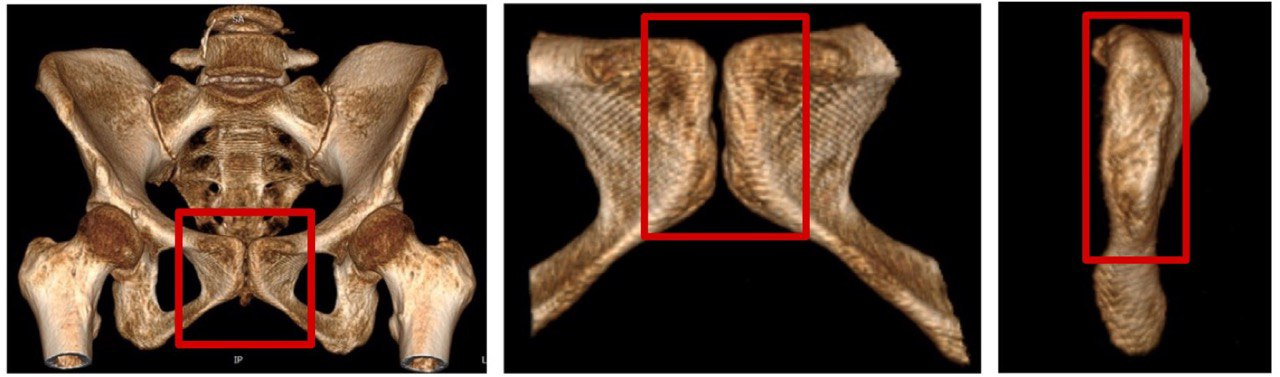
\includegraphics[width=\textwidth]{imagenes/pubis.jpg}
    \caption[Reconstrucción volumétrica por tomografía computerizada 3D de la sínfisis del pubis.]{Reconstrucción volumétrica por tomografía computerizada 3D de la sínfisis del pubis en RadiAnt \cite{hisham2019quantification}. Las imágenes no tienen la misma escala. \textbf{Izquierda}: Pelvis humana. \textbf{Centro}: Ampliación de ambas partes del pubis. \textbf{Derecha}: Cara del pubis izquierdo. Encuadrado en rojo se ha marcado la sínfisis púbica.}
    \label{fig:pubis}
\end{figure}

Como podemos apreciar en la Figura \ref{fig:pubis}, la sínfisis del pubis es la conexión entre las dos partes del pubis. Esta puede observarse tanto en la cara del pubis derecho como del izquierdo. Es en estas caras donde los antropólogos forenses centran su atención a la hora de identificar características morfológicas. Estas características, discriminatorias y observables a simple vista, fueron descritas por T. W. Todd en su artículo \textbf{\textit{Ages changes in the pubic bone}} (1921) \cite{todd1921age}. Aún a día de hoy, 100 años después de la publicación de este artículo, los antropólogos forenses localizan y emplean las características descritas por Todd a la hora de estimar la edad de los restos óseos de personas muertas en edad adulta. Entre dichas características se encuentran: la porosidad, definición y profundidad de las crestas y surcos; la porosidad y regularidad de la superficie y la presencia de nódulos o bordes; entre otras. En la Figura \ref{fig:toddfeatures} podemos ver un ejemplo de algunas de las características definidas por Todd.

\begin{figure}[ht!]
    \centering
    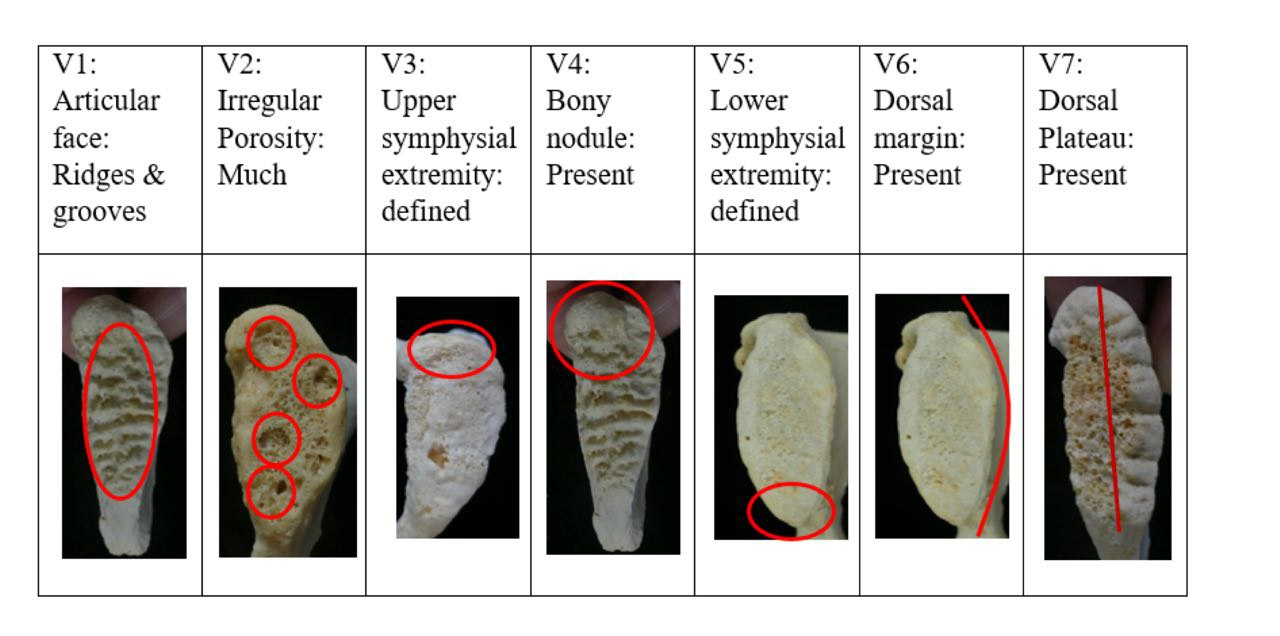
\includegraphics[width=\textwidth]{imagenes/Toddfeatures.jpg}
    \caption[Características morfológicas en la sínfisis púbica.]{Algunos ejemplos de características que definen el desarrollo típico y los cambios morfológicos degenerativos en la sínfisis púbica durante el crecimiento. Las regiones de interés están resaltadas en rojo}
    \label{fig:toddfeatures}
\end{figure}

Todd también estableció varios rangos de edad para los que los restos óseos presentaban características similares. Como se puede observar en la Tabla \ref{tab:rangosTodd} estos rangos o fases abarcan de 1 o 2 años para muestras jóvenes (18-26 años) a 4 años de diferencia en las últimas fases. Además el último rango de edad es catalogado como 50 años o más. Esto era adecuado para la época de publicación del artículo, pero queda bastante obsoleto en el momento actual en el que la esperanza de vida es superior.\\ 
% Estos rangos o fases son los siguientes:
% \begin{itemize}
%     \item Fase 1: 19 años
%     \item Fase 2: 20 a 21 años
%     \item Fase 3: 22 a 24 años
%     \item Fase 4: 25 a 26 años
%     \item Fase 5: 27 a 30 años
%     \item Fase 6: 31 a 34 años
%     \item Fase 7: 35 a 39 años
%     \item Fase 8: 40 a 44 años
%     \item Fase 9: 45 a 49 años
%     \item Fase 10: 50 años o más
% \end{itemize}


% % Please add the following required packages to your document preamble:
% % \usepackage{graphicx}
% \begin{table}[ht!]
% \centering
% \begin{tabular}{|l|l|}
% Fase 1 & 19 años \\
% Fase 2 & 20 a 21 años \\
% Fase 3 & 22 a 24 años \\
% Fase 4 & 25 a 26 años \\
% Fase 5 & 27 a 30 años \\
% Fase 6 & 31 a 34 años \\
% Fase 7 & 35 a 39 años \\
% Fase 8 & 40 a 44 años \\
% Fase 9 & 45 a 49 años \\
% Fase 10 & 50 años o más
% \end{tabular}%
% \caption{Intervalos de edad de la muerte propuestos por Todd.}
% \label{tab:rangosTodd}
% \end{table}

% Please add the following required packages to your document preamble:
% \usepackage{graphicx}
\begin{table}[ht!]
\centering
\begin{tabular}{|l|l|l|l|}
\hline
\textbf{Fase 1} & 19 años & \textbf{Fase 6} & 31 a 34 años \\ \hline
\textbf{Fase 2} & 20 a 21 años & \textbf{Fase 7} & 35 a 39 años \\ \hline
\textbf{Fase 3} & 22 a 24 años & \textbf{Fase 8} & 40 a 44 años \\ \hline
\textbf{Fase 4} & 25 a 26 años & \textbf{Fase 9} & 45 a 49 años \\ \hline
\textbf{Fase 5} & 27 a 30 años & \textbf{Fase 10} & 50 años o más \\ \hline
\end{tabular}%
\caption{Intervalos de edad de la muerte propuestos por Todd.}
\label{tab:rangosTodd}
\end{table}

Para realizar el proceso de estimación de la edad a partir de restos humanos, podemos diferenciar dos enfoques distintos: realizar la estimación aportando un valor continuo para la edad de la muerte, como el enfoque propuesto por Gilbert-McKern \cite{gilbert1973method}, o determinar la edad en un intervalo, como los enfoques propuestos por el propio Todd \cite{todd1921age} o el propuesto por Suchey-Brooks \cite{brooks1990skeletal}. En el estado del arte actual ha habido diversos intentos de automatizar estos métodos de estimación de la edad (ver Capítulo \ref{chap:estadodelarte}). Los métodos de automatización propuestos han aplicado diversos métodos de aprendizaje automático (regresores, modelos Bayesianos, redes neuronales, etc.) consolidados en cuanto a resolución de problemas de clasificación y regresión.\\

Sin embargo, en este proyecto proponemos un nuevo enfoque. Aplicar técnicas de \textbf{aprendizaje profundo} (DL) a la tarea de la estimación de la edad a partir de las sínfisis púbicas. Lo haremos, además, sin tomar como base ninguno de los métodos de extracción de características morfológicas actuales, si no que será el propio modelo quién aprenderá a extraer estas características de forma automática.
Como datos de entrada contaremos con el conjunto de modelos 3D de las sínfisis púbicas humanas escaneadas manualmente por personal del laboratorio de Antropología Física del Departamento de Medicina Legal, Toxicología y Antropología Física de la Universidad de Granada. Por tanto, el desarrollo del proyecto presenta un reto doble. En primer lugar, el uso de modelos 3D en el campo del DL supone un reto en sí mismo, ya que no existen precedentes en su aplicación en el campo de la medicina legal. En segundo lugar, las técnicas de DL aplicadas deben extraer automáticamente características morfológicas discriminatorias de los modelos 3D de las sínfisis púbicas sin la intervención de un experto humano. Todo ello configura un TFG de enorme originalidad y carácter disruptivo, en donde se presenta una propuesta transgresora en relación al resto de modelos y técnicas existentes en el estado del arte. Los resultados proporcionados por la propuesta de este TFG se compararán con aquellos obtenidos con métodos pre-existentes. \\

% La combinación de estas dos características aporta un enfoque totalmente transgresor a la propuesta presentada, ya que no existe ninguna propuesta similar en el estado del arte. Además, de forma que podamos estimar la bondad de los resultados obtenidos estos se compararán con los resultados aportados por los métodos presentes en el estado del arte.\\

% Aquí hay un salto muy brusco. Pasas de repente de Todd, que es un método manual de estimación de fases, a que vas a usar Deep Learning. Debes meter uno o dos párrafos intermedios, que digan que hay métodos que estiman las fases y otros que estiman directamente la edad. Luego que últimamente se están aplicando métodos automáticos, algunos de los cuales usan las características de Todd y otros no. Sería un breve resumen de lo que hay en la sección 3.1.1.

% Por último, que vamos a proponer una variante transgresora, en la que se usa DL para estimar la edad numérica sin haber detectado características a priori, y que vamos a validar su rendimiento con respecto al estado del arte basado en métodos de distintos tipos de entre los anteriores.

% Todo lo comentado hasta aquí me parece que está bien y es muy interesante. Pero creo que falta remarcar la importancia de hacerlo en 3D y de modo automático. Es decir, creo que falta un poco remarcar la contribución de este TFG, que es perfectamente publicable porque es un investigación científica realmente novedosa. Por ejemplo, cosas que echo un poco de menos: 
% - indicar que ha habido ciertos intentos de automatizar Todd (luego, ya se mencionarán en detalle estos intentos en Estado del Arte). Mencionar dichos intentos y dar alguna pincelada. 
% - mencionar que este es el primer trabajo que opera, ya no con imágenes 2D (que no sé si hay otros trabajos tampoco), con modelos 3D. Algo que, ya en sí mismo, dentro de DL es novedoso. 
% - también estaría bien, para entender un poco mejor en qué consiste Todd, incluir alguna figura o figuras mostrando el tipo de características en que se fijan los antropólogos de cara a a aplicar el método. 

Finalmente, en base a todo lo anteriormente descrito y a modo de resumen, el presente TFG aborda la tarea de \textbf{estimar la edad de un individuo mediante la aplicación de técnicas de DL a modelos 3D de la sínfisis púbica}.
\newpage
%%%%%%%%%%%%%%%%%%%%%%%%%%%%%%%%%%%%%%%%%%%%%%%%%%%%%%%%%%%%%%%%%%%%%%%%%%%%%%%%%%%%%%%%%%%
\section{Motivación}
Los antropólogos forenses utilizan las características macroscópicas descritas en \cite{todd1921age} para poder realizar una estimación de la edad de los restos analizados. La extracción de estas características (ver Figura \ref{fig:toddfeatures}) depende en gran medida de la experiencia y criterio del antropólogo que realiza el análisis. Esto en ocasiones puede concurrir en errores a la hora de realizar una estimación correcta de la edad de unos restos.\\

Actualmente uno de los principales retos a los que se enfrenta la AF es responder con precisión, robustez y rapidez al enorme número de casos que deben ser abordados. La estimación de la edad de restos óseos es una tarea fundamental en casos de personas desaparecidas, accidentes múltiples, incendios, desastres naturales, actos de terrorismo, fosas comunes, crímenes de lesa humanidad\footnote{Se considera crímenes de lesa humanidad —o contra la humanidad— a aquellos delitos especialmente atroces y de carácter inhumano, que forman parte de un ataque generalizado o sistemático contra una población civil, cometidos para aplicar las políticas de un Estado o una organización.}, etc \cite{ubelaker2008forensic, ubelaker2020recent}. Por esto la minimización de los errores cometidos por los antropólogos forenses en el proceso de ID es clave.\\

A continuación se muestran algunos ejemplos donde la estimación del PB y la aplicación de técnicas de AF resultan indispensables:

\begin{itemize}
    \item Según el Centro Nacional de Desaparecidos (CNDES), desde el año 2011 han sido hallados 2.749 cadáveres o restos humanos sin identificar en España. De estos solo han podido ser identificados 656.
    
    \item Según datos ofrecidos por el Ministerio del Interior, en España hay en la actualidad 12.330 casos de personas desaparecidas sin resolver.
    
    \item Según el Ministerio de Justicia, en España se han contabilizado 2.457 fosas comunes. En estas,  la Plataforma de Víctimas de Desapariciones Forzadas por el Franquismo estima que fueron enterradas más de 140.000 personas víctimas de ejecuciones extrajudiciales y asesinatos en custodia durante el período de 1936 a 1975.
    
    \item En junio de 2019 había contabilizados en España por el Ministerio del Interior un total de 12.301 menores migrantes no acompañados (MENAS). Entre los motivos que llevan a estos niños y niñas a salir de sus países de origen se encuentran la pobreza y la falta de futuro y expectativas; situaciones de desestructuración familiar y desprotección institucional; catástrofes naturales; la guerra, la persecución, la violencia y situaciones de violación generalizada de los derechos humanos.
    
    \item Según los cálculos de la Agencia de la ONU para los Refugiados (ACNUR), para fines de noviembre de 2021 la cantidad de personas muertas o desaparecidas en travesías a través del Mediterráneo ya superaba los 2500.
    
    \item Entre 2017 y 2020 a nivel mundial murieron 970 personas como consecuencia de ataques terroristas.
    
    \item En 2020, el número de víctimas mortales registradas a nivel mundial como consecuencia de las catástrofes naturales ascendió a aproximadamente 8.200. La AF tiene un papel fundamental en sucesos de víctimas múltiples, siendo responsable de la individualización de fragmentos, comparación radiográfica, estimación del PB, etc. 
    
    \item La AF está fuertemente vinculada a la investigación de crímenes de lesa humanidad, siendo la principal responsable de la identificación de personas como consecuencia de desapariciones forzadas, ejecuciones extrajudiciales, masacres y otras formas de violencia. 
    
\end{itemize}

A pesar de estos dramáticos datos, y del consiguiente interés humanitario, político y social que existe a la hora de resolver muchos de estos casos, sorprende constatar el bajo desarrollo tecnológico de la AF en comparación con otras disciplinas médicas \cite{mesejo2020survey}. Aún a día de hoy, las herramientas más utilizadas por los antropólogos forenses para el desempeño de su práctica diaria son el calibre y la hoja de cálculo.\\

Como ingenieros, tenemos la capacidad de dotar a la sociedad con herramientas que ayuden a desempeñar tareas complejas de forma que los errores cometidos por el factor humano sean mínimos. Existen numerosos ejemplos de sistemas de inteligencia artificial que adaptan métodos basados en el análisis esquelético para desempeñar la tarea de estimar el PB de un individuo \cite{mesejo2020survey}.\\

Además en años recientes, las técnicas de DL aplicadas directamente sobre modelos 3D han aportado buenos resultados en resolución de tareas como clasificación de objetos, recuperación de la pose y segmentación \cite{ahmed2018survey,gezawa2020review}. Dado que la tendencia dentro de la AF es que los antropólogos forenses trabajen cada vez más con modelos 3D de los restos óseos en lugar de trabajar directamente con estos, un sistema capaz de asistir en la tarea de la estimación de la edad a partir de la información obtenida de forma automática directamente de estos modelos 3D podría ser una herramienta de gran utilidad para los antropólogos forenses, guiándolos a la hora de realizar su labor.\\

La motivación de este TFG viene dada por la necesidad de dotar a los antropólogos forenses de herramientas para el apoyo en la estimación de la edad de restos humanos.\\
%%%%%%%%%%%%%%%%%%%%%%%%%%%%%%%%%%%%%%%%%%%%%%%%%%%%%%%%%%%%%%%%%%%%%%%%%%%%%%%%%%%%%%%%%%%

%%%%%%%%%%%%%%%%%%%%%%%%%%%%%%%%%%%%%%%%%%%%%%%%%%%%%%%%%%%%%%%%%%%%%%%%%%%%%%%%%%%%%%%%%%%
\section{Objetivos}

El objetivo general de este proyecto es, como se ha comentado anteriormente, estimar la edad de un individuo mediante la aplicación de técnicas de DL a modelos 3D de la sínfisis púbica. Para esto definiremos un modelo que extraiga la información necesaria para realizar la estimación directamente a partir de los modelos 3D. Para poder desarrollar este modelo, encontraremos una representación de la información de los modelos 3D entre las opciones disponibles en el estado del arte. En la Figura \ref{fig:modelo} vemos un esquema de la propuesta presentada.\\

\begin{figure}[ht!]
    \centering
    \includegraphics[width=\textwidth]{imagenes/objetive.drawio.png}
    \caption{Representación del modelo a desarrollar.}
    \label{fig:modelo}
\end{figure}

Para el desarrollo de este TFG, dividiremos el objetivo general en los siguientes objetivos parciales:
\begin{itemize}
    \item Dado que la fuente principal de datos se trata de una serie de modelos 3D, realizaremos un análisis pormenorizado y sistemático de las formas presentes en el estado del arte de representación de datos en 3D. De todas las formas existentes, enumeraremos las ventajas y desventajas de cada una, eligiendo finalmente una única forma de representar los datos.
    \item Desarrollaremos las herramientas necesarias para poder implementar la representación de los datos.
    \item Diseñaremos un modelo de red neuronal profunda que permita trabajar con la representación de datos 3D. 
    \item Comprobaremos si la representación de la información escogida y el modelo desarrollado permiten aprender de forma automática y satisfactoria las características representativas de los restos óseos, de forma que la estimación del modelo pueda servir como apoyo para el trabajo de un antropólogo forense. Para esto, compararemos los resultados obtenidos con aquellos aportados por los métodos actuales presentes en el estado del arte.
\end{itemize}

Para ajustarnos a estos objetivos, y documentar el trabajo realizado de la forma más clara y completa posible, esta memoria se estructura de la siguiente forma: en el Capítulo \ref{chap:fundamentos} presentaremos los fundamentos teóricos en los que se basa el desarrollo del proyecto; en el Capítulo \ref{chap:estadodelarte} analizaremos el estado del arte tanto para la estimación de la edad a partir de restos óseos como para la representación de datos 3D en el ámbito del DL; en el Capítulo \ref{chap:metodologia} presentaremos los métodos utilizados para desarrollar los objetivos propuestos; en el Capítulo \ref{chap:planyimpl} se proporcionarán detalles sobre la planificación y la implementación del proyecto, en el Capítulo \ref{chap:experimentos} veremos el protocolo de validación experimental del modelo y el proceso de entrenamiento del mismo, y analizaremos los resultados finales obtenidos y los compararemos con el estado del arte y, finalmente, en el Capítulo \ref{chap:conclusiones} presentaremos las conclusiones principales de este TFG.
\chapter{Fundamentos teóricos}
\label{chap:fundamentos}

Esta sección tiene como objetivo presentar y explicar los fundamentos teóricos en los que se basan los métodos utilizados en el desarrollo de este proyecto, así como justificar su relevancia en la resolución del problema que se plantea.

\section{Machine learning}

El \textbf{machine learning} (ML) o \textbf{aprendizaje automático} \cite{bishop2006pattern,alpaydin2020introduction,abu2012learning} es una rama de la inteligencia artificial centrada en el uso de datos y algoritmos para desarrollar y entender modelos que sean capaces de aprender patrones existentes en los datos de forma progresiva. 
La forma en que estos modelos aprenden es mejorando gradualmente su rendimiento al resolver una tarea o problema concretos.

Los modelos de ML pueden aprender a partir de datos de cualquier tipo: números, palabras, estadísticas, imágenes, etc. 
Cualquier información almacenada digitalmente puede utilizarse como entrada para un modelo.
Los modelos aprenden información de los patrones extraídos de los datos de entrenamiento, mejorando su rendimiento con el tiempo. 
Una vez entrenado, un modelo podrá identificar los patrones aprendidos en nuevos datos, distintos a los utilizados en el proceso de entrenamiento.

Estos modelos tienen una amplia variedad de aplicaciones: visión por computador, reconocimiento del lenguaje natural, aplicaciones en el campo de la medicina, filtrado automático de contenido, etc. 
Son particularmente útiles en tareas que no pueden ser abordadas por algoritmos convencionales.\\

Diferenciamos tres aproximaciones o problemáticas principales dentro del ML: aprendizaje supervisado, aprendizaje no supervisado y aprendizaje por refuerzo.\\
\newpage
El \textbf{aprendizaje supervisado} consiste en presentar los datos de entrenamiento como un conjunto de datos de entrada (\textit{inputs}) etiquetados con la información que debe determinar (\textit{output}). Está aproximación requiere un menor número de datos de entrenamiento y facilita el proceso de aprendizaje, ya que los resultados obtenidos por el modelo pueden compararse con los datos ya etiquetados. Sin embargo, este proceso de etiquetado puede ser costoso, ya que hay que conocer previamente como se deben etiquetar los datos para que el modelo pueda aprender y aplicar el conocimiento adquirido en la clasificación de nuevos datos. Además, el modelo es muy sensible al etiquetado de datos, pudiendo obtener modelos sesgados en función al etiquetado de los datos de entrenamiento.
Las problemáticas de aprendizaje supervisado incluyen algoritmos de clasificación y regresión. Los algoritmos de clasificación se aplica en tareas donde las etiquetas están limitadas a un conjunto de valores discretos, mientras que los de regresión se aplican en casos en los que las etiquetas presentan un dominio continuo de valores.\\

A diferencia del aprendizaje supervisado, en el \textbf{aprendizaje no supervisado} los datos de entrada no se encuentran etiquetados. Esta aproximación se centra en la identificación de patrones y relaciones existentes en el conjunto de datos de entrenamiento, de forma que pueda etiquetar y clasificar los datos sin la intervención humana. Requiere un mayor número de datos y es menos utilizada frente a otras aproximaciones. El aprendizaje semi-supervisado es un enfoque intermedio que consiste en utilizar un subconjunto de datos etiquetado para guiar la extracción y detección de patrones en el conjunto no etiquetado.\\

Finalmente, el \textbf{aprendizaje por refuerzo} se basa en determinar las acciones que debe llevar a cabo un algoritmo o agente en un determinado entorno, con el objetivo de maximizar la recompensa acumulada. El agente es recompensando positiva o negativamente en función de su desempeño. Esta técnica se aplica en campos como los algoritmos genéticos o la teoría de juegos.\\

Aunque estas tres problemáticas son las principales, existen muchas aproximaciones distintas como el aprendizaje débilmente supervisado, auto-supervisado, multitarea, etc. Muchas de estas reúnen características de varias aproximaciones, como es el caso del aprendizaje semi-supervisado. Las aproximaciones que hemos comentado no son departamentos estancos, por lo que un algoritmo de ML puede ubicarse en varias de ellas en función de como se aborde el problema a resolver.
\newpage
\section{Deep learning}
El \textbf{deep learning} (DL) o \textbf{aprendizaje profundo} \cite{lecun2015deep,schmidhuber2015deep,goodfellow2016deep} es un subcampo del ML. Los métodos de DL tienen como objetivo obtener representaciones más abstractas (en ultima instancia, más útiles) mediante la combinación de múltiples transformaciones no lineales \cite{bengio2013representation}. ML y DL difieren en cómo aprende cada algoritmo. DL automatiza el proceso de extracción de características de los datos, eliminando la intervención humana y consiguiendo que los algoritmos de DL sean aplicables en conjuntos de datos mucho mayores. También se puede entender el DL como una versión escalable del ML clásico \cite{ibm_cloud_education_2020}. El ML depende en gran medida de la intervención de un experto en el conjunto de datos capaz de extraer las características del mismo. Los métodos empleados en DL pueden aplicarse en conjuntos de datos etiquetados, de la misma forma que se aplicarían los métodos de ML, sin embargo, no es una condición necesaria. Los modelos DL pueden extraer conjuntos de características discriminatorias para elementos de distinta clase a partir de datos en bruto como texto o imágenes.

\subsection{Redes neuronales}
\label{sec:redes_neuronales}

Las \textbf{redes neuronales} \cite{bishop1995neural}, también conocidas como redes neuronales artificiales (ANN), son un subcampo del ML y forman el núcleo del DL. Su nombre y su estructura toma inspiración del cebero humano. Se busca imitar la forma en que las neuronas biológicas interactúan entre sí.

Las redes neuronales están formadas por capas de nodos: una capa de entrada, una o varias capas de nodos ocultas y una capa de salida. Cada neurona (o nodo) se conecta a las de la capa siguiente como puede verse en la Figura \ref{fig:redesneuronales}. Esta conexión tiene un peso y un umbral de activación asociado. Si el valor de salida de un nodo es superior al umbral de activación, la información se transmite hacia delante entre las capas de nodo. De lo contrario esta información no se transmite entre las capas. Los valores producidos como salida de una red neuronal pueden ser tanto valores continuos, binarios o categorías especificas en función de la tarea que se desee realizar.\\

\begin{figure}[ht!]
    \centering
    \includegraphics[width=\textwidth]{imagenes/RedesNeuronales.png}
    \caption[Ejemplo de red neuronal superficial y profunda.]{Ejemplo de red neuronal superficial y profunda \cite{garcía_iñareta_j_o_2020}.}
    \label{fig:redesneuronales}
\end{figure}

Cada conexión entre dos nodos tiene un peso asignado, de forma que se modela la \say{fuerza} de cada una de las señales de entrada a un nodo. El correcto ajuste de estos pesos será el que permitirá a la red neuronal aprender a realizar la tarea que debe llevar a cabo. Los datos introducidos a la capa de entrada que pueden verse en la Figura \ref{fig:neurona} se definen como variables independientes. Serán procesados por el siguiente nodo para propagar la información hacia delante en la red. Todas las variables independientes de la red corresponden a una única muestra del conjunto de datos disponible. La forma en la que los datos se procesan en los nodos es multiplicando las señales de entrada por el peso asignado a cada señal y combinando linealmente estas operaciones. Posteriormente a esta combinación lineal se le aplica una función de activación.\\

Las funciones de activación son una parte fundamental de las redes neuronales, pues son las que introducen la no linealidad en el modelo y en última instancia, permiten a la red aprender. De aplicarse funciones de activación lineales, la red sería equivalente a una red sin capas ocultas. Las funciones de activación más comunes suelen ser la función threshold, la función sigmoide, la función rectificadora (ReLU) y la función tangente hiperbólica. Sin embargo existen más funciones de activación distintas a las mencionadas. La elección de una función de activación u otra esta motivada por el problema a resolver y por los resultados experimentales obtenidos.

\begin{figure}[ht!]
    \centering
    \includegraphics[width=\textwidth]{imagenes/Neurona_Completa.png}
    \caption[Procesamiento de señal a nivel de nodo.]{Procesamiento de señal a nivel de nodo \cite{garcía_iñareta_j_o_2020}.}
    \label{fig:neurona}
\end{figure}

Además de la función de activación, otra función imprescindible a la hora de hablar de redes neuronales es la función de pérdida o función de error. Ya hemos comentado que el objetivo de la red neuronal es ajustar los pesos asociados a sus conexiones de forma que el resultado final obtenido sea el resultado deseado. Para medir la diferencia entre el resultado obtenido y el resultado deseado establecemos una función de pérdida. El valor obtenido por esta función será utilizado para realizar un ajuste en los pesos del modelo en un proceso conocido como \say{backpropagation}. La información de la función de pérdida se transmite desde la última capa de la red hacia la capa inicial. De nuevo, la función de perdida utilizada dependerá del objetivo a desempeñar y de los resultados experimentales. Existen funciones específicas para regresión como la función error absoluto medio (MAE) y la función error cuadrático medio (MSE). También hay funciones específicas para tareas de clasificación como la función de entropía cruzada de categorías (Categorical CrossEntropy) o la función de entropía cruzada binaria (Binary CrossEntropy).\\

El proceso iterativo de propagar la información de la capa de entrada a través de los nodos, procesar esta información mediante combinaciones lineales de las señales y la aplicación de funciones de activación, evaluar la función de pérdida y realizar backpropagation para ajustar los pesos del modelo se conoce como entrenamiento de una red neuronal. Según avanza este proceso iterativo, el objetivo de la red es minimizar el valor de la función de pérdida.\\

Es importante tener en cuenta que una red neuronal puede sobreaprender los datos de entrada, incurriendo en un fenómeno conocido como \say{overfitting} (al igual que otros modelos dentro del campo del ML). El \say{overfitting} o sobreajuste se produce cuando la red neuronal es capaz de clasificar los datos de entrenamiento con una precisión muy alta, pero sin embargo al intentar clasificar nuevos datos diferentes a los de entrenamiento, la red no consigue generalizar correctamente y su desempeño es mucho menor. Para esto existen procesos de regularización que están diseñados para evitar que se produzca sobreajuste en el modelo.

\subsection{Redes neuronales convolucionales}

Las \textbf{convolutional neural networks} (CNN) o redes neuronales convolucionales \cite{lecun1989backpropagation,lecun1998gradient} son un tipo de algoritmo de DL, concretamente una subclase de las redes neuronales. Estas redes están diseñadas para trabajar con imágenes como dato de entrada\footnote{Generalmente es así, pero existen arquitecturas de CNN específicas para modelos 3D y otro tipo de datos.}. Son capaces de detectar las regiones características capaces de diferenciar las imágenes que reciben como input a partir de los pesos de la red. El preprocesado necesario en este tipo de redes es mucho menor que en el de otros modelos, ya que son capaces de aprender y desarrollar filtros capaces de detectar las características discriminatorias de una imagen.\\

La arquitectura de este tipo de redes es análoga al patrón de conexión entre neuronas de las redes neuronales clásicas. Las CNN son capaces de capturar las dependencias temporales y espaciales presentes en una imagen mediante la aplicación de filtros relevantes que la red aprende en el proceso de entrenamiento. El objetivo de las CNN es reducir las imágenes de forma que se facilite el proceso de aprendizaje sin perder características discriminatorias de las mismas. Esto favorece a que este tipo de redes sean escalables a conjuntos de datos masivos.

\subsubsection{Capa de convolución}

El operador de \textbf{convolución} es la base de las CNN (ver Figura \ref{fig:conv}). Una convolución es un operador matemático que transforma dos funciones $f$ y $g$ en una tercera función que representa la magnitud en la que se superponen $f$ y una versión invertida y trasladada de $g$. En el caso de las CNN, estas funciones $f$ y $g$ se tratan de una imagen (I) y un kernel o filtro (K) respectivamente. El kernel se desplaza por la imagen calculando la convolución entre la sección de la imagen correspondiente y el kernel (ver Figura \ref{fig:kernelmov}). El kernel se desplaza hacia la derecha con determinado valor de salto (\say{stride}) hasta que se completa la primera fila. Después el kernel comienza a desplazarse de la misma manera por las siguientes filas comenzando desde la izquierda. Este proceso continua hasta que el kernel pasa por toda la imagen. En el caso de imágenes con más de un canal, el kernel tiene la misma profundidad que la imagen y el resultado de la convolución es una imagen con un único canal que se compone de la suma de la convolución de cada canal con el kernel.

\begin{figure}[ht!]
    \centering
    \includegraphics[width=0.5\textwidth]{imagenes/conv.png}
    \caption[Operación de convolución.]{Operación de convolución \cite{saha_2018}.}
    \label{fig:conv}
\end{figure}

\begin{figure}[ht!]
    \centering
    \includegraphics[width=0.25\textwidth]{imagenes/KernelMovement.png}
    \caption[Movimiento del kernel sobre la imagen.]{Movimiento del kernel sobre la imagen \cite{saha_2018}.}
    \label{fig:kernelmov}
\end{figure}

El objetivo de la capa de convolución es extraer características de alto nivel presentes en la imagen. Generalmente la primera capa convolucional es responsable de extraer características de bajo nivel \cite{saha_2018} como colores, bordes, gradiente de orientación, etc. Según se van añadiendo capas de convolución, la arquitectura se adapta para extraer también características de alto nivel. Esta combinación de varias capas convolucionales, proporciona a la red un entendimiento completo de las imágenes del conjunto de datos.\\

Hay dos posibles resultados tras aplicar la convolución a una imagen, esta puede o reducir sus dimensiones o mantener las mismas. Este resultado se controla mediante la aplicación de \say{\textbf{padding}} o rellenado. El padding consiste en aumentar las dimensiones de la imagen, introduciendo información redundante o rellenando el nuevo espacio con ceros, de forma que la imagen resultado de la convolución no pierda tamaño.

\subsubsection{Capa de pooling}

Al igual que la capa de convolución, la capa de \say{\textbf{pooling}} o agrupación se encarga de reducir la dimensión espacial de las convoluciones realizadas. La reducción de la dimensionalidad contribuye a reducir el coste computacional necesario para procesar los datos de entrada. Además la capa de pooling sirve para extraer las características dominantes que son invariantes a rotaciones y a la posición, manteniendo la efectividad en el proceso de entrenamiento de la red.\\

Los dos tipos de pooling más utilizados son: \textbf{max pooling} (agrupación máxima) y \textbf{average pooling} (agrupación media). El max pooling consiste en conservar el valor máximo de la sección de la imagen cubierta por el kernel. Además aplicar max pooling contribuye a suprimir ruido presente en la imagen. Descarta las activaciones provocadas por ruido mientras produce una reducción de la dimensionalidad. El average pooling por otro lado, consiste en obtener la media de los valores de la sección de la imagen cubierta por el kernel. El average pooling suprime el ruido presente en la imagen simplemente consiguiendo una reducción de la dimensionalidad. Un ejemplo de ambos tipos de pooling puede verse en la Figura \ref{fig:pooling}.

\begin{figure}[ht!]
    \centering
    \includegraphics[width=0.5\textwidth]{imagenes/pooling2.png}
    \caption[Tipos de pooling.]{Tipos de pooling \cite{yani2019application}.}
    \label{fig:pooling}
\end{figure}

La composición de capas de convolución y pooling forman la base de las CNN. Aumentando y reduciendo su número, puede controlarse la extracción de características de mayor o menor nivel en función de la complejidad de la imagen de entrada. Sin embargo, un mayor número de capas conllevará un mayor coste computacional en el procesado de los datos.

\subsubsection{Capa densa o totalmente conectada}

Una vez terminado el proceso de aplicación de convolución y pooling, los datos procesados se reducen a un único vector de características que se utiliza como entrada para una red neuronal clásica que se encarga de realizar la clasificación, regresión o la tarea que se desee (ver Figura \ref{fig:fc}).
Podemos entender las CNN como una red neuronal formada por dos bloques principales: uno de convolución y pooling, que actúa como extractor automático de características y otro bloque formado por una red neuronal clásica, que utiliza las características extraídas para cumplir con el objetivo de la red.\\

En las CNN, las capas en las que los nodos están totalmente conectados, en una arquitectura análoga a una red neuronal clásica, se las conoce como capas \textbf{densas}, \textbf{totalmente conectadas} o \say{\textbf{fully connected}}. Esta es una forma sencilla de conseguir que el modelo aprenda combinaciones no lineales de las características obtenidas en las capas de convolución y pooling.\\

% La salida de esta capas, es el resultado final de la CNN, que será evaluado por una función de perdida. En función del resultado de aplicar esta función, se llevará a cabo un proceso de backtracking que actualizará los pesos de las conexiones entre nodos así como los valores de los filtros utilizados en las convoluciones. El proceso de entrenamiento de una CNN es análogo al entrenamiento de una red neuronal clásica.
La salida de esta capas, es el resultado final de la CNN, que será evaluado por una función de perdida. Se llevará a cabo un proceso de backpropagation que actualizará los pesos de las conexiones entre nodos así como los valores de los filtros utilizados en las convoluciones, con el objetivo de minimizar el valor de la función de pérdida utilizada. El proceso de entrenamiento de una CNN es análogo al entrenamiento de una red neuronal clásica.

\begin{figure}[ht!]
    \centering
    \includegraphics[width=0.75\textwidth]{imagenes/cnn.png}
    \caption[Arquitectura de CNN.]{Arquitectura de CNN en la que pueden apreciarse las capas de convolución, pooling y totalmente conectada o densa \cite{saha_2018}.}
    \label{fig:fc}
\end{figure}

\subsubsection{Batch normalization y dropout}
Como hemos comentado en la sección \ref{sec:redes_neuronales}, durante el proceso de entrenamiento de una CNN puede producirse un fenómeno conocido como \say{overffiting}. Este fenómeno impide a la CNN generalizar correctamente la información aprendida, por lo que el desempeño de la red fuera de los datos de entrenamiento se reduce drásticamente. Para evitar el overfitting, existen estrategias que pueden aplicarse en las redes neuronales clásicas y en las CNN. Aquí nos centraremos en dos de ellas, batch normalization y dropout.\\

El \textbf{batch normalization} (normalización de subconjunto) es un método algorítmico que permite que el entrenamiento de la CNN sea más rápido y más estable. En la práctica consiste en una capa que se encarga de normalizar los vectores de activación de las capas ocultas de la red. Para esto utiliza la media y la varianza de cada \say{batch} de datos. El concepto de batch en las CNN hace referencia al número de datos que se introducen a la red antes de que se produzca el proceso de backpropagation y la actualización de los pesos de la red. Batch normalization tiene un efecto regularizador en la red, por lo que contribuye a prevenir el overfitting.\\

El \textbf{dropout} (abandono) es una técnica de regularización en redes neuronales. Consiste en \say{apagar} nodos aleatorios (tanto de las capas ocultas como de las visibles) durante el proceso de entrenamiento (ver Figura \ref{fig:dropout}). Esto se consigue omitiendo el valor de los nodos en función de una probabilidad concreta. La aplicación del dropout consigue que la red entrenada sea más robusta \cite{nelson_2018}, ya que permite que la red aprenda correctamente evitando la posibilidad de que varios nodos compensen los errores de otros en el proceso de entrenamiento.

\begin{figure}[ht!]
    \centering
    \includegraphics[width=0.75\textwidth]{imagenes/dropout.png}
    \caption[Ejemplo de aplicación de dropout.]{Ejemplo de aplicación de dropout. \textbf{Izquierda}: Red completa. \textbf{Derecha}: Red tras la aplicación de dropout \cite{budhiraja_2018}.}
    \label{fig:dropout}
\end{figure}

\section{Tipos de representación de datos en 3D}
\label{sec:datos3d}

La aplicación de técnicas de DL en visión por computador ha estado generalmente dirigida al uso de datos 2D. En este campo se han obtenido numerosos resultados en tareas de clasificación, reconocimiento, segmentación, etc. La principal ventaja de los modelos DL es su capacidad para aprender progresivamente características jerárquicas de los datos proporcionados como entrada \cite{krizhevsky2012imagenet}. Sin embargo estos modelos requieren una gran cantidad de datos para su entrenamiento. Debido a esto, el uso de modelos DL en datos 3D ha estado limitado. En los últimos años, debido al avance de la tecnología en escaneo 3D, al abaratamiento y mejor accesibilidad de la misma, la cantidad de datos 3D disponibles para entrenamiento ha aumentado notablemente. Ejemplos como la popularidad del Kinect o el desarrollo de los sensores LIDAR han contribuido a eso.
\\

Los algoritmos utilizados en modelos DL orientados a datos 3D deben afrontar principalmente dos desafíos: la representación de estos modelos 3D y la estructura de red utilizada. En esta sección abordaremos el primero de estos desafíos analizando las representaciones existentes de datos 3D, sus ventajas y desventajas y su posible aplicación en la estimación del PB.
\\

Según la literatura consultada, existen varias formas de categorizar los tipos de datos 3D. Gezawa et al. \cite{gezawa2020review} distinguen en su estudio 5 grandes categorías: datos en bruto, superficies, solidos, estructuras de alto nivel y múltiples vistas. Esta distinción se basa en la forma de adquisición de los datos y la estructura interna de los mismos. Por otro lado Ahmed et al. \cite{ahmed2018survey} dividen los tipos de datos 3D en euclideanos y no euclideanos. Los datos euclideanos cuentan con una estructura de \say{rejilla} subyacente que permite una parametrización global de los datos y establecer un sistema de coordenadas común. Los datos no euclideanos no cuentan con esta estructura subyacente, por lo que no existe parametrización global. En la Tabla \ref{tab:comparativa} vemos un representación esquemática de estas categorías y las diferentes formas de representar los datos 3D que pertenecen a cada una de ellas.
\\

% Please add the following required packages to your document preamble:
% \usepackage{multirow}
% \usepackage[table,xcdraw]{xcolor}
% If you use beamer only pass "xcolor=table" option, i.e. \documentclass[xcolor=table]{beamer}
\begin{table}[ht!]
\centering
\begin{tabular}{c|c|l|}
\cline{2-3}
\multicolumn{1}{l|}{}                                                                               & \textbf{Euclideano}                           & \multicolumn{1}{c|}{\textbf{No Euclideano}} \\ \hline
\multicolumn{1}{|c|}{}                                                                              & RGB-D \cite{rgbd}                                        & \multicolumn{1}{c|}{Nubes de puntos \cite{memoli2005theoretical}}        \\ \cline{2-3} 
\multicolumn{1}{|c|}{\multirow{-2}{*}{\textbf{Datos en bruto}}}                                     & Proyecciones 3D \cite{projecciones3D}                              & \cellcolor[HTML]{C0C0C0}                    \\ \hline
\multicolumn{1}{|c|}{}                                                                              & Octrees \cite{voxelsoctrees}                                      & \cellcolor[HTML]{C0C0C0}                    \\ \cline{2-3} 
\multicolumn{1}{|c|}{\multirow{-2}{*}{\textbf{Sólidos}}}                                            & Vóxeles \cite{voxelsoctrees}                                      & \cellcolor[HTML]{C0C0C0}                    \\ \hline
\multicolumn{1}{|c|}{\textbf{Superficies}}                                                          & \multicolumn{1}{l|}{\cellcolor[HTML]{C0C0C0}} & \multicolumn{1}{c|}{Malla 3D \cite{bronstein2021geometric}}               \\ \hline
\multicolumn{1}{|c|}{\textbf{\begin{tabular}[c]{@{}c@{}}Estructuras de \\ alto nivel\end{tabular}}} & Descriptores 3D \cite{descriptors3D}                              & \multicolumn{1}{c|}{Grafos \cite{bronstein2021geometric}}                 \\ \hline
\multicolumn{1}{|c|}{\textbf{\begin{tabular}[c]{@{}c@{}}Datos de \\ múltiples vistas\end{tabular}}} & Múltiples vistas \cite{multiview}                             & \cellcolor[HTML]{C0C0C0}                    \\ \hline
\end{tabular}
\caption{Diferentes clasificaciones para los distintos tipos de datos 3D.}
\label{tab:comparativa}
\end{table}

\subsection{Datos en bruto}
Dentro de la categoría de datos en bruto se agrupan representaciones que utilizan datos directamente obtenidos del positivo de captura obtenido, aplicando transformaciones simples o directamente no aplicando ninguna transformación. Podemos encontrar los datos RGB-D, las proyecciones 3D y las nubes de puntos. %Los dos primeros presentan una estructura euclideana mientras que las nubes de puntos son más complicadas de clasificar.

\subsubsection{Datos RGB-D}
Los datos RGB-D representan la información de los datos en 2.5 dimensiones. Están formados por una imagen clásica de 2 dimensiones (RGB) a la que se añade un mapa de profundidad (D) que aporta el valor de profundidad captado por el sensor para cada píxel. Es una representación simple pero efectiva. 
\\

La principal ventaja de esta representación es la sencillez en su obtención (ya que los dispositivos utilizados, como Kinect, tienen gran disponibilidad) y su facilidad de aplicación a modelos DL preparados para 2D existentes. Su principal desventaja es que, dado que la representación RGB-D no contiene la totalidad de la geometría del objeto 3D, los modelos utilizados no podrán aprender la geometría completa de dicho objeto, por lo que solo se podrán inferir algunas propiedades 3D en base a la profundidad. Esto ha motivado a los investigadores a explorar otras técnicas de representación de datos. 

\subsubsection{Proyecciones 3D}
Proyectar puntos 3D en un espacio 2D es otra forma de representar de datos 3D. La proyección encapsula información clave del objeto 3D original. Comúnmente las proyecciones más utilizadas son las proyección cilíndricas y esféricas. Estas últimas poseen la ventaja de proporcionar invarianza a la rotación en el eje principal de la proyección. 
\\

Su principal ventaja es que dado que la proyección contiene información clave del objeto 3D original, es posible utilizar modelos de DL clásicos para trabajar con datos 3D. La principales desventajas son que la aplicación directa de esta representación en modelos DL en 2D requiere un mayor ajuste fino y que al proyectar datos 3D en un espacio 2D las propiedades geométricas de la forma del objeto 3D original se pierden. Por esto, muchos investigadores han tratado de utilizar varias proyecciones en conjunto o combinar esta representación con otras para compensar esta falta de información. Pese a sus desventajas, la utilización de este tipo de representación 3D en modelos DL ha probado ser eficaz a la hora de aprender formas 3D. 

\subsubsection{Nubes de puntos}
Una nube de puntos no es más que un conjunto no estructurado de puntos 3D que aproximan la geometría de objetos 3D en el que cada punto esta representado por tres coordenadas. Aunque las nubes de puntos pueden obtenerse fácilmente (utilizando dispositivos cono Kinect o sensores LIDAR) su procesamiento puede ser un desafío debido a la falta de información de conectividad entre los puntos que forman la nube. También puede darse el caso en que debido a las condiciones de adquisición de los datos, ciertos puntos no se representen correctamente, las nubes representen información incompleta o se introduzca ruido en los datos, provocando pérdidas de información.
\\

Si podemos pasar por alto estos inconvenientes, las nubes de puntos presentan varias ventajas. Estas proveen una representación expresiva, homogénea y compacta de la geometría de la superficie 3D con mucha menor complejidad respecto a otras representaciones como mallas 3D o grafos. Su principal desventaja a la hora de procesar los datos es la estructura desordenada y no uniforme que presentan, debido a los errores derivados de la adquisición de los datos. Esto ha llevado a los investigadores a desarrollar métodos de aprendizaje que sean invariantes al orden de los puntos dentro de la nube.

\subsection{Sólidos}
En esta categoría encontramos representaciones de los datos 3D que simplemente proporcionan información de control del espacio ocupado por un objeto determinado. Generalmente dicha información es binaria, lo que significa que un punto del espacio puede estar ocupado o no. Dentro de esta categoría encontramos representaciones con vóxeles y octrees.

\subsubsection{Vóxeles}
Los vóxeles modelan los datos 3D describiendo como el objeto 3D se distribuye en el espacio tridimensional. La información que proporciona el punto de vista también puede ser codificada clasificando los vóxeles ocupados en visibles u ocluidos.
\\

La principal ventaja es que proporciona información volumétrica de la totalidad del objeto 3D que se representa. Sin embargo, esta representación presenta una gran desventaja: requiere una enorme cantidad de memoria, ya que se deben almacenar todos los vóxeles independientemente de si son visibles o no. Por esto, la representación en vóxeles no es adecuada para representar objetos 3D con resoluciones altas. Cuanto mayor sea la resolución, mayor será el almacenamiento necesario.

\subsubsection{Octrees}
Como una forma más eficiente de representación de la información volumétrica de objetos 3D, surgen los octrees (arboles octales). Un octree es simplemente una estructura de representación de información espacial basada en vóxeles de tamaño variable. Los octrees se construyen como árboles de los que cada nodo cuelgan ocho nodos diferentes \cite{tatarchenko2017octree} que dividen el espacio 3D en cubos que pueden estar tanto dentro como fuera del objeto.
\\

Sus principales ventajas son la eficiencia en la utilización de la memoria y su capacidad para generar vóxeles de alta resolución \cite{riegler2017octnet}. Por otro lado, su principal desventaja es que presenta una incapacidad para mantener la geometría de algunos objetos 3D como la suavidad de la superficie, por ejemplo.

\subsection{Superficies}
Las superficies de polígonos se suelen utilizar en la representación de los límites de los objetos 3D que rodean la parte interior del objeto. El conjunto de estos polígonos suele almacenarse para la descripción
del objeto, lo que tiene la ventaja de la simplicidad y la rapidez de la representación de la superficie y de la visualización del objeto dado que todas superficies se pueden caracterizar con ecuaciones lineales. Dentro de esta categoría solo encontramos las mallas 3D.

\subsubsection{Mallas 3D}
Las mallas 3D son una de las representaciones más populares de objetos 3D. Consisten en una combinación de vértices, aristas y caras que se utilizan generalmente se utilizan gráficos por ordenador para renderizado y almacenamiento de modelos 3D. Los vértices se asocian con una lista de conectividad que describen como estos se interconectan entre ellos. La complejidad e irregularidad de estas mallas provocan que no hayan sido utilizadas con técnicas DL orientadas a modelos 3D hasta ahora.
\\

Su principal ventaja es que se trata de una de las representaciones de datos 3D más importantes y potentes dentro de su campo. Esto ha propiciado su amplio uso dentro del campo de los gráficos por ordenador. Su principal desventaja es la ya comentada complejidad e irregularidad de las mallas 3D. El estudio de la aplicación de estas mallas al campo del DL continua avanzando a día de hoy, por lo que los modelos actuales son bastante recientes además de computacionalmente costosos.

\subsection{Estructuras de alto nivel}
En problemas de clasificación de objetos 3D, a veces es necesaria una representación concisa y detallada. Dentro de las estructuras de alto nivel, podemos encontrar descriptores 3D de alto nivel y grafos.

\subsubsection{Descriptores 3D}
Los descriptores de forma son representaciones simplificadas de objetos 3D que describen características geométricas o topológicas de los mismo. Estos descriptores pueden obtenerse a partir de elementos del objeto 3D tales como la geometría, topología, superficie, textura o cualquier otra, siendo posible también utilizar una combinación de todas ellas \cite{zhang2007survey,kazmi2013survey}. Un descriptor de forma puede entender como una \say{firma} de la forma del objeto 3D para facilitar el procesamiento y computación así como facilitar la comparación entre diferentes objetos. 
Estos descriptores normalmente se combinan con un modelo basado en el aprendizaje para extraer características jerárquicas discriminatorias para representar el objeto 3D de mejor forma.
Los descriptores 3D se clasifican en 2 categorías: descriptores locales y globales. Los descriptores globales proporcionan información del objeto 3D en su totalidad, mientras que los locales proveen una representación de una zona concreta del modelo.
\\

Como principales ventajas encontramos que los descriptores 3D pueden codificar mucha información relativa a un modelo 3D de forma simple. Por esto han sido ampliamente utilizamos en el campo del DL. Sin embargo, su principal desventaja es que un descriptor demasiado simple puede conllevar una pérdida de las propiedades del modelo que esta representando.
\\

Además revisando la literatura, la mayoría de aplicaciones de los descriptores 3D se centran en el paradigma del aprendizaje no supervisado. Esto se debe a que los modelos de aprendizaje supervisado aprenden abstracciones jerárquicas de los datos en bruto. Dado que los descriptores 3D son en si mismos una abstracción, su aplicación en modelos de aprendizaje supervisado podría derivar en no obtener características representativas. El proceso de aprendizaje de abstracciones a partir de abstracciones puede llevar a una pérdida de las propiedades actuales de los modelos 3D representados si el descriptor 3D utilizado es demasiado simple o abstracto. Sin embargo  en algunos casos, los descriptores pueden proveer información lo suficientemente completa como para que la operación de convolución pueda aprender características jerárquicas de los datos de entrada \cite{han2016mesh}.

\subsubsection{Grafos}
La representación por grafos de un objeto 3D recoge la esencia de la geometría del objeto enlazando diferentes partes del modelo mediante un grafo. Las mallas 3D son extensiones de datos estructurados en forma de grafos, en los que los nodos del grafo se utilizan como los vértices de la malla y las aristas representan las conexiones entre los vértices \cite{fey2018splinecnn}. Los primeros acercamientos a redes neuronales convoluciones para grafos, Graph Convolutional Neural Networks (GNN), aplican principalmente dos operadores de convolución distintos: métodos de filtrado espectral y métodos de filtrado espacial. Aunque ambos métodos son equivalentes aunque se fundamentan en principios matemáticos diferentes, por lo que presentan varias diferencias.\\

Los métodos de filtrado espectral se fundamentan en la descomposición en vectores y valores propios de la matriz laplaciana de un grafo \cite{flawnsontong2019}. Esto se conoce como descomposición espectral de un grafo \cite{hammond2011wavelets}. Esta descomposición se utiliza para definir un operador de convolución. Los métodos de filtrado espectral son robustos, fiables y tienen un amplio recorrido en la bibliografía. Sin embargo son métodos matemáticos complejos que conllevan costes computacionales más elevados. Además son dependientes de la base del grafo utilizado lo que hace que la generalización de estos modelos sea aún objeto de estudio.\\

Por otra parte, los métodos de filtrado espacial se basan en que dentro de un modelo de GNN, el aprendizaje de las características que definen a un grafo depende del vecindario de cada vértice. De forma análoga a las CNN clásicas, un función no lineal se aplica a todos los nodos del grafo. La elección de esta varía en función de la tarea. Los métodos de filtrado espacial son menos complejos que los de filtrado espectral, pero no por ello menos potentes. La principal diferencia radica en que los métodos espaciales combinan los vectores de características de los vecindarios de vértices basándose en la topología del grafo y considerando su estructura espacial.


\subsection{Datos de múltiples vistas}
Los datos 3D pueden representarse como una combinación de múltiples imágenes 2D generadas como diferentes puntos de vista del objeto 3D \cite{zhao2017multi}. 
\\

Esta representación permite el aprendizaje de múltiples conjuntos de características para reducir posibles efectos de ruido, oclusión, estado incompleto de los datos y cambios de iluminación generados por el proceso de captura de los datos. Además, permite trabajar con entradas de alta resolución, pues pueden aplicarse modelos DL basados en imágenes 2D. El aprendizaje de datos 3D a partir de múltiples imágenes 2D del objeto, aspira a aprender una función capaz de modelar cada vista por separado para después optimizar conjuntamente todas las funciones aprendidas de forma que pueda representarse el objeto 3D en su totalidad además de generalizar la representación de otros objetos 3D. Sin embargo, su mayor inconveniente es establecer el número de vistas suficientes para representar el objeto 3D. Un número de vistas demasiado bajo puede producir que no se capturen las propiedades del objeto 3D en su totalidad y además podría conllevar un problema de overfitting. Por otro lado, un número de vistas muy elevado podría incrementar innecesariamente el coste computacional. Además el uso de este tipo de representación no es capaz de preservar las características geométricas intrínsecas de los modelos 3D.\\

A modo de resumen, en la Figura \ref{fig:rep3D} vemos varios ejemplos de las diferentes formas de representación de los datos 3D presentadas en esta sección.

\newpage

\begin{figure}[ht!]
    \centering
    \includegraphics[width=\textwidth]{imagenes/Representaciones3D.png}
    \caption[Diferentes formas de representación de los datos 3D.]{Diferentes formas de representación de los datos 3D \cite{gezawa2020review}.}
    \label{fig:rep3D}
\end{figure}
\chapter{Estado del arte}
\label{chap:estadodelarte}

\section{Estimación del perfil biológico}
% En el contexto de la AF y más concretamente, en el desempeño de la tarea de la estimación del PB, existen dos escenarios posibles. El más común es que el antropólogo forense tenga acceso directo a los restos óseos para poder realizar la estimación. Estos son extraídos, limpiados y manipulados directamente por el mismo. Un segundo escenario se presenta cuando el antropólogo forense no tiene acceso directo a los restos. Para estos casos existen otras aproximaciones basadas en métodos menos invasivos y adecuados para casos en los que la estimación del PB (sobre todo edad biológica) deba realizarse en individuos vivos \cite{mesejo2020survey}.\\

En el contexto de la AF y más concretamente en el desempeño de la tarea de la estimación del PB, existen dos escenarios posibles. Esta puede realizarse tanto para individuos fallecidos, a través de sus restos óseos, en casos de identificación de cadáveres; como para individuos vivos, en casos de personas desaparecidas o menores no acompañados que solicitan asilo fuera de su lugar de origen.\\

La estimación de la edad es un tema que ha ido tomando relevancia a lo largo del tiempo. En la Figura \ref{fig:publicaciones} podemos ver como el número de publicaciones relacionadas con esta tarea, enmarcada dentro de la AF, ha ido aumento año tras año hasta superar más de 100 publicaciones en los últimos años. Sin embargo, en dicha figura también podemos ver como el número de publicaciones relacionadas con la estimación de la edad y la AF que hagan mención a la inteligencia artificial o al aprendizaje automático no es un tema tan popular. Los métodos automáticos (métodos que hacen usos de técnicas de inteligencia artificial) han comenzado a surgir desde mediados de la década y actualmente no se supera la veintena de publicaciones sobre el tema. Por esto, se remarca la importancia de este proyecto, aplicar un nuevo enfoque a la estimación de la edad a partir de restos óseos de forma automática.\\

\begin{figure}[ht!]
    \centering
    \includegraphics[width=\textwidth]{imagenes/n_publicaciones.pdf}
    \caption[Número de publicaciones relacionadas con la estimación de la edad y la AF por año.]{Número de publicaciones relacionadas con la estimación de la edad y la AF por año. \textbf{Azul}: cualquier publicación relacionada con este campo. \textbf{Rojo}: publicaciones que contienen referencias a aprendizaje automático o inteligencia artificial}
    \label{fig:publicaciones}
\end{figure}

Para el desarrollo de esta sección, nos centraremos en el escenario de la estimación de la edad en individuos fallecidos a partir de sus restos óseos. Analizaremos el estado del arte de las técnicas actuales tanto manuales como automáticas. Además centraremos nuestra atención en los métodos que estiman la edad mediante el uso de sínfisis púbicas.


\subsection{Estimación de la edad a partir de restos óseos}

Realizar esta estimación sobre restos humanos de individuos adultos es una tarea compleja. En la AF existen diferentes métodos aplicables en base a la evolución del proceso degenerativo normal de los restos \cite{ubelaker2020recent}. Las regiones anatómicas más útiles para llevar a cabo la estimación son aquellas que no se ven afectadas por factores externos como el trabajo o la actividad física.
Los métodos basados en el uso de sínfisis púbicas \cite{todd1921age,brooks1990skeletal,hartnett2010analysis}, la superficie auricular del ilium \cite{buckberry2002age} y el extremo esternal de la cuarta costilla \cite{icscan1984metamorphosis} han mostrado una buena precisión en la estimación de la edad. El análisis del desarrollo y proceso degenerativo del hueso púbico es el método más extendido y esta reconocido como una de las alternativas más fiables \cite{cunha2009problem,dudzik2015estimating}.

\subsection{Estimación de la edad a partir de la sínfisis púbica}
Los primeros estudios para la estimación de la edad (edad de muerte) mediante el análisis de restos de las sínfisis del pubis fueron los realizados por  T. W. Todd en 1921 \cite{todd1921age}. Todd analizó 360 esqueletos de varones caucásicos en un rango de entre 18 y 60 años para establecer 10 rangos de desarrollo y progreso degenerativo. Para establecer estas fases, Todd definió una descripción morfológica de la sínfisis púbica para cada edad.\\

Aunque existen criticas al método diseñado por Todd, aún 100 años después de la publicación original de \cite{todd1921age}, las características y criterios morfológicos descritos son utilizados a día de hoy como metodología recomendada.\\

Debemos distinguir dos tipos de enfoques en los métodos de estimación de la edad basados en el uso de las sínfisis púbicas. Los métodos que proporcionan una estimación de la edad de la muerte en un intervalo o fase (métodos basados en fases) y los métodos que proveen una estimación de un valor específico para la edad de la muerte de un individuo (métodos numéricos).
En función de como estos métodos estimen la edad, podemos diferenciar métodos que estiman un valor para cada rasgo o componente por separado y posteriormente combinan las diferentes estimaciones (métodos basados en componentes) o métodos que realizan una estimación de forma global.\\

Actualmente uno de los métodos más recomendados para la estimación de la edad a partir de sínfisis púbicas es el propuesto por Suchey y Brooks \cite{brooks1990skeletal}. Este método es una adaptación de la propuesta de Todd. Suchey y Brooks reducen el número de fases a 6 y modifican los rangos de edad, ampliándolos y superponiéndolos entre ellos. Sin embargo, la forma de aplicar el método seguía siendo prácticamente la misma que la propuesta por Todd: la evaluación subjetiva de las características morfológicas de la sínfisis púbica y la asignación manual de una fase de edad de la muerte por parte de un antropólogo forense.
\\

Como alternativa a los métodos basados en fases, Gilbert y McKern \cite{gilbert1973method} fueron posiblemente los primeros en considerar un análisis independiente de cada uno de los componentes. Su propuesta se basaba en un sencillo sistema de regresión, que utilizaba una variable continua para la edad de la muerte, obtenida mediante la suma del valor asociado a cada componente por separado (p.ej. las características de la sínfisis púbica). Este valor asociado a las componentes es asignado por un antropólogo forense tras una inspección visual. Aunque el método de Gilbert-McKern no funcionó correctamente, se convirtió en el punto de partida del criticismo hacia los métodos basados en fases por parte de muchos autores en las décadas siguientes.
\\

A pesar de las adaptaciones propuestas sobre el método de Todd, este método y sus variantes como la de Suchey y Brooks y la de Gilbert y McKern se aplican de forma rutinaria de forma similar a la de la propuesta original. Esto significa que la valoración de los rasgos morfológicos de la sínfisis púbica y su correspondencia con el estándar de cada fase es una valoración subjetiva y depende de la experiencia del antropólogo forense. Por lo tanto, la principal desventaja de estos métodos es la subjetividad presente tanto en la descripción morfológica de las sínfisis púbicas como en la elección de la fase de desarrollo y proceso degenerativo a la que pertenece \cite{dudzik2015estimating}. Esta subjetividad se deriva de la falta de sistematización del método, el cual ofrece descripciones demasiado genéricas que dificultan la discriminación entre fases. En la Tabla \ref{tbl:3dmodelsTodd} podemos apreciar un ejemplo de modelos 3D pertenecientes a cada una de las fases descritas por Todd.\\

\begin{table}[h!]
  \centering
  \resizebox{\linewidth}{!}{%
  \begin{tabular}{ | c | c | c | c | c |}
    \hline
    Fase 1 & Fase 2 & Fase 3 & Fase 4 & Fase 5 \\ \hline
    \begin{minipage}{.3\textwidth}
      \includegraphics[width=\linewidth, height=60mm]{imagenes/modelfase1.png}
    \end{minipage}
    &
    \begin{minipage}{.3\textwidth}
      \includegraphics[width=\linewidth, height=60mm]{imagenes/modelfase2.png}
    \end{minipage}
    & 
    \begin{minipage}{.3\textwidth}
      \includegraphics[width=\linewidth, height=60mm]{imagenes/modelfase3.png}
    \end{minipage}
    & 
    \begin{minipage}{.3\textwidth}
      \includegraphics[width=\linewidth, height=60mm]{imagenes/modelfase4.png}
    \end{minipage}
    & 
    \begin{minipage}{.3\textwidth}
      \includegraphics[width=\linewidth, height=60mm]{imagenes/modelfase5.png}
    \end{minipage}
    \\ \hline
    Fase 6 & Fase 7 & Fase 8 & Fase 9 & Fase 10 \\ \hline
    \begin{minipage}{.3\textwidth}
      \includegraphics[width=\linewidth, height=60mm]{imagenes/modelfase6.png}
    \end{minipage}
    &
    \begin{minipage}{.3\textwidth}
      \includegraphics[width=\linewidth, height=60mm]{imagenes/modelfase7.png}
    \end{minipage}
    & 
    \begin{minipage}{.3\textwidth}
      \includegraphics[width=\linewidth, height=60mm]{imagenes/modelfase8.png}
    \end{minipage}
    & 
    \begin{minipage}{.3\textwidth}
      \includegraphics[width=\linewidth, height=60mm]{imagenes/modelfase9.png}
    \end{minipage}
    & 
    \begin{minipage}{.3\textwidth}
      \includegraphics[width=\linewidth, height=60mm]{imagenes/modelfase10.png}
    \end{minipage}
    \\ \hline
  \end{tabular}
  }
  \caption{Ejemplos de modelos 3D de sínfisis púbicas pertenecientes a cada una de las fases de Todd.}
  \label{tbl:3dmodelsTodd}
\end{table}

Los métodos de estimación de la edad a partir de restos óseos deberían ofrecer el mismo resultado independientemente del experto que lo aplique. Sin embargo, numerosos estudios han demostrado que la efectividad de estos métodos dependen casi exclusivamente de la experiencia del antropólogo forense \cite{schmitt2002variability,kimmerle2008inter}. Ante esta situación, es necesario utilizar métodos que reduzcan la subjetividad de los procesos de estimación de la edad. El uso de técnicas de IA como algoritmos de ML y DL o inteligencia artificial explicable (XAI) en la AF puede beneficiar este área ampliando los métodos existentes y extendiendo su aplicación desde expertos antropólogos a practicantes.\\

Diferentes métodos por ordenador se han considerado con el propósito de objetivizar (y automatizar en algunos casos) la estimación de la edad de la sínfisis del pubis. Los principales avances han ido encaminados a sustituir el estudio directo del hueso por el estudio de modelos 3D digitalizados, ya sea utilizando nuevos criterios o los criterios utilizados en los métodos originales \cite{dedouit2007virtual}.\\

Dentro de los métodos basados en fases encontramos varias propuestas presentadas por equipos de investigación de la Universidad de Granada.\\

En \cite{villar2017first}, Villar et al. modelan el problema como una tarea de clasificación de ML clásico con 10 fases independientes de edad. Los principales rasgos morfológicos del hueso descritos por Todd fueron analizados y modelados como nueve variables lingüísticas basadas en el conocimiento de expertos forenses. Dos antropólogos forenses distintos etiquetaron manualmente un pequeño conjunto de sínfisis púbicas de 74 individuos. Se obtuvieron bases de reglas compactas compuestas por entre 17 y 20 reglas utilizando árboles de decisión difusos. Estos reportaron un un error medio absoluto (MAE) ordinal de 1.07 en todo el conjunto y 1.68 en el conjunto de test mediante validación cruzada en 10 iteraciones. Sin embargo las reglas derivadas no cubrían todas las fases, por lo que el proceso de validación no era totalmente fiable debido a las limitaciones del conjunto de datos (pequeño y no equilibrado) y el enfoque de ML seguido.\\

En \cite{gámez_irurita_gonzález_damas_alemán_cordón_2021}, Gámez-Granados et al. diseñan un sistema explicable y basado en reglas para estimar la edad de la muerte a parir de sínfisis púbicas evocando el conocimiento del método de Todd y su procedimiento. Este método considera nueve características del hueso púbico basadas en las descripciones de Todd y extraídas por antropólogos forenses. Dado que el conjunto de datos utilizado estaba fuertemente desbalanceado, consideran el de sobremuestreo de datos y un algoritmo de aprendizaje de reglas de clasificación ordinal (NSLVOrd \cite{gamez2016ordinal}). El modelo entrenado aporta un error cuadrático medio (RMSE) de 12,34 años y un MAE de 10,38 años en una muestra con 892 huesos del pubis, considerando los valores intermedios de los rangos de edad de las fases de Todd. Hasta el momento es el mejor resultado del estado del arte en cuanto a métodos semi-automáticos basados en fases.\\

Por otro lado dentro de los métodos que estiman directamente la edad de la muerte, encontramos diversos autores que consideran diferentes técnicas de regresión y técnicas de inteligencia artificial para desarrollar nuevos métodos.\\

En \cite{slice2015modeling}, Slice y Algee-Hewitt introducen SHA, un índice para cuantificar la variación de la morfología de la superficie de la sínfisis púbica asociada al envejecimiento en el método de Todd. Se calcula a partir de un análisis de componentes principales (PCA) de los modelos 3D escaneados por láser. SHA se utiliza para diseñar un modelo de regresión lineal evaluado en un estudio que considera 41 esqueletos de varones americanos. \cite{slice2015modeling} obtiene un rendimiento similar a Suchey-Brooks \cite{brooks1990skeletal}, reportando RMSE de 17,15 años.\\ %Los mismos autores presentan una mejora de su método en \cite{stoyanova2015enhanced} considerando una sola característica extraída automáticamente a partir de modelos 3D de las sínfisis púbicas, la flexión de un plano para que este coincida con la superficie del hueso. Un modelo de regresión lineal que estima directamente el valor numérico de la edad de la muerte a partir de una sola variable obtiene un RMSE de unos 19 años en una muestra similar de 56 sujetos en el rango de entre 16 y 100 años. Por último, este equipo introduce dos modelos finales basados en una regresión multivariable haciendo uso de un nuevo conjunto de rasgos que integra características adicionales basadas en la curvatura extraídas de los modelos 3D. Estos modelos finales aportan de un RMSE en el rango de 13,7-16,5 años en una muestra de 93 individuos varones blancos de entre 16 y 90 años.\\

Más adelante en \cite{stoyanova2015enhanced}, Stoyanova et al. diseñan otro modelo lineal que estima la edad a partir de una única variable extraída automáticamente a partir de los modelos 3D de las sínfisis del pubis, la energía de flexión (bending energy). Este enfoque se prueba con 44 esqueletos escaneados de varones blancos documentados y 12 moldes en representación de las fases de Suchey-Brooks \cite{brooks1990skeletal} en el rango de entre 16 y 100 años, reportando un RMSE de aproximadamente 19 años. En \cite{stoyanova2017computational} amplían su anterior trabajo extrayendo nuevas características en base a la curvatura del modelo 3D e integrándolas todas en dos modelos de regresión multivariante. Este trabajo se evalúa en un conjunto de 93 modelos 3D de varones blancos entre 16 y 90 años (68 reales y 25 moldes) obteniendo un RMSE de entre 13,7 y 16,5.\\

En \cite{kotverova2018age}, Koterova et al. proponen nueve métodos de regresión automática para la estimación de la edad. En su propuesta, combinan tres rasgos de la sínfisis púbica con cuatro de la superficie auricular del ilium. Estos métodos se validan en un conjunto de datos de 941 individuos multiétnicos de adultos entre 19 y 100 años. Se consideraron enfoques de regresión clásica, K-NN vecinos cercanos, modelos Bayesianos, arboles de regresión y redes neuronales. La regresión multlineal fue el mejor de los predictores, aportando un RMSE de 12,1 años y un MAE de 9,7 años.\\

En \cite{dudzik2015estimating}, Dudzik y Langley se centran en la incertidumbre que surge de las definiciones de los rasgos óseos y la dificultad de los antropólogos para entenderlas. Se analizan las características óseas en las etapas previas a los cambios degenerativos avanzados en 237 individuos americanos. La regresión logística multinomial y los arboles de decisión se aplican sobre una muestra de 47 individuos jóvenes en el rango de edad de entre 18 y 40 años, utilizando cinco rasgos de la sínfisis púbica. Reportan un 94\% de precisión, pero considerando solo 3 fases distintas.\\

En \cite{villegas_TFG}, Bermejo et al. proponen un nuevo enfoque semi-automático basado en componentes a partir de los rasgos morfológicos de las sínfisis púbicas propuestos por Todd. Este método se basa en la obtención de en una expresión matemática que combina los valores de de los distintos componentes, proporcionados por el experto forense, en un valor numérico para la edad de la muerte. Se consideran métodos de ML explicables, haciendo uso de la programación genética para derivar dichas fórmulas a partir de los datos de la base de datos pública disponible en el Laboratorio de Antropología Física de la Universidad de Granada. Se sigue un enfoque de ciencia de datos guiado por la teoría \cite{karpatne2017theory} que combina la experiencia del antropólogo forense y las descripciones explicables derivadas de los datos. Se proponen dos enfoques, uno aplica técnicas de programación genética (GP) y el otro combinando esto con algoritmos genéticos (GA-P). Ambos enfoques aportan resultados de RMSE 10,81 y MAE 8,55.
\\

Finalmente en \cite{castillo2021preliminary}, Castillo et al. proponen un nuevo método basado en fases y en componentes diseñado utilizando métodos de ML. Con el objetivo de manejar tanto la variación interindividual como la subjetividad de los sistemas de puntuación visual, su marco considera 16 rasgos diferentes de la sínfisis púbica, incluyendo uno novedoso que no ha sido utilizado previamente (microranuras). Todos ellos sólo presentan dos valores categóricos (presente o ausente) para facilitar la tarea de etiquetado al antropólogo forense. Se aplica un método de selección de características sobre cada uno de las 5 fases de edad de la muerte analizadas para seleccionar las mejores características considerando para ello tres algoritmos diferentes de ML (ZeroR, Naïve Bayes y Random Forest). Los autores muestran resultados muy prometedores para algunas fases de edad así como una discriminación entre características útiles e inútiles.\\

En la Tabla \ref{tab:state_of_art_estimacion} podemos ver un resumen de los resultados presentes en el estado del arte introducidos en esta sección.
% Please add the following required packages to your document preamble:
% \usepackage{graphicx}
\begin{table}[ht!]
\centering
\resizebox{\textwidth}{!}{%
\begin{tabular}{|l|l|c|c|c|c|}
\hline
\textbf{Método} & \textbf{Tipo} & \textbf{N muestras} & \textbf{Rango de edad} & \textbf{RMSE} & \textbf{MAE} \\ \hline
Slice y Algee-Hewitt \cite{slice2015modeling} & N, CS & 41 & 19 - 96 & 17,15 & - \\ \hline
Stoyanova et al. \cite{stoyanova2015enhanced} & N, CS & 56 & 16 - 100 & 19 & - \\ \hline
Stoyanova et al. \cite{stoyanova2017computational} & N, CS & 93 & 16 - 90 & 13,7 - 16,5 & - \\ \hline
Koterova et al. \cite{kotverova2018age} & N, CS & 941 & 19 - 100 & 12,1 & 9,7 \\ \hline
Gámez-Granados et al. \cite{gámez_irurita_gonzález_damas_alemán_cordón_2021} & PB, G & 892 & 18 - 60 & 13,19 & 10,38 \\ \hline
Gámez-Granados et al. \cite{gámez_irurita_gonzález_damas_alemán_cordón_2021} & PB, G & 960 & 18 - 60 & 14,61 & 11,62 \\ \hline
Bermejo et al \cite{villegas_TFG} (GP) & N, CS & 1152 & 18-82 & 10,82 & 8,56 \\ \hline
Bermejo et al \cite{villegas_TFG} (GA-P) & N, CS & 1152 & 18-82 & \textbf{10,81} & \textbf{8,55} \\ \hline
\end{tabular}%
}
\caption[Resumen de los resultados presentes en el estado del arte de los métodos de estimación de la edad.]{Resumen de los resultados presentes en el estado del arte de los métodos de estimación de la edad. \textbf{Tipo}: PB, basado en fases; N, numérico; CS, basado en componentes; G, global. \textbf{MAE} y \textbf{RMSE} indican el error medido en años.}
\label{tab:state_of_art_estimacion}
\end{table}

%\section{Técnicas de Deep Learning para representación de datos en 3D}

\section{Representación de datos 3D}

En la Sección \ref{sec:datos3d} se han introducido todas las opciones para representar datos 3D utilizadas actualmente en el paradigma del DL. En esta sección haremos un análisis de cuáles son las más adecuadas para la utilización en la estimación de la edad mediante el uso de sínfisis púbicas.
\\

En primer lugar descartamos la representación RGB-D. Dado que los modelos de los que se dispone son modelos 3D completos especificados como una lista de vértices y aristas, se produciría una pérdida de información geométrica al utilizar esta representación. Descartaremos también el uso de representaciones volumétricas (vóxeles y octrees). Este tipo de representaciones se centran en proporcionar información sobre como el modelo 3D ocupa el espacio. Los vóxeles requieren un uso elevado de memoria para representar datos en alta resolución. Los octrees por otro lado, aunque no tienen el problema de usar demasiada memoria, no pueden capturar correctamente propiedades del modelo 3D como la morfología de la superficie. Dado que esta propiedad puede proporcionar información fundamental de la que se podrán extraer características discriminatorias, la representación con vóxeles y octrees de los modelos 3D conllevaría grandes pérdidas de información.
\\

Por tanto las posibles opciones se reducen a: proyecciones 3D, nubes de puntos, mallas 3D, descriptores 3D, grafos y múltiples vistas. Descartamos los descriptores 3D debido a que los resultados obtenidos dependerán de la capacidad del descriptor escogido de codificar correctamente la información geométrica de los modelos 3D. Dado que los modelos 3D empleados poseen un alto nivel de detalle, sería necesario utilizar un descriptor muy potente. Además, dado que las características que permiten estimar la edad de las sínfisis púbica se encuentran bien definidas \cite{todd1921age}, se ha decidido optar por un modelo que no dependa de una representación codificada. De esta forma el modelo podrá extraer las características directamente de los datos y estas podrán compararse con las definidas por Todd. \\

% \sout{En cuanto a las proyecciones 3D, también las descartamos debido a que en el proceso de proyección de los puntos del modelo 3D al plano 2D podría producirse perdida de información geométrica.}

Descartamos también las nubes de puntos dado que estas son similares a la representación de grafos y mallas pero eliminando el componente de conectividad de los puntos. Por esto, si utilizamos esta representación se estaría eliminando información útil necesaria para el proceso de estimación de la edad. Finalmente descartamos la representación en múltiples vistas, pues aunque estas codifican información de modelos 3D, el objetivo de este proyecto es trabajar directamente con los datos 3D como entrada del modelo.
\\

% \sout{Descartadas estas opciones solo nos queda la representación en grafos y en mallas 3D. Estas dos representaciones son muy similares entre si, dado que una malla 3D puede verse también como un grafo no dirigido G = (V,E) tal que V esta formada por los vértices de la malla y E por las aristas. Por esto se mantendrá la estructura de malla 3D de los modelos 3D, pero se utilizará un modelo de Geometric Deep Learning (GDL) para realizar la estimación.}

Descartadas estas opciones solo nos quedan las proyecciones 3D, la representación en grafos y la representación en mallas 3D. Estas últimas son muy similares entre si, dado que una malla 3D puede verse también como un grafo no dirigido G = (V,E) tal que V esta formada por los vértices de la malla y E por las aristas. Se barajó el uso de modelos de geometric deep learning (GDL), que utilizan mallas 3D como entrada de datos. Sin embargo, estos tienen grandes inconvenientes. Los ejemplos disponibles en la literatura actual trabajan con mallas 3D formadas por un número limitado de polígonos. Dado que los datos disponibles para entrenamiento, cuentan con una media de 1.000.000 de polígonos\footnote{La media de polígonos de los datos de entrenamiento es 1.001.507,08}. Para poder procesar modelos con una definición tan alta, sería necesario calcular una malla simplificada para cada modelo 3D, con menor número de polígonos. Esto conllevaría una perdida de información geométrica del modelo, pero de no realizarse, sería imposible entrenar el modelo con el hardware disponible. Por ello, la representación en mallas 3D/grafos queda descartada.\\

% La representación utilizada será una basada en proyecciones 3D, que se desarrollará con mayor detalle en el Capítulo \ref{chap:metodologia}.

Finalmente, queda como última opción la representación haciendo uso de proyecciones 3D. Esta representación puede ser muy versátil, ya que su aplicación es compatible con el uso de modelos y arquitecturas de DL clásico que han mostrado ser muy competitivas a la hora de resolver tareas de clasificación y regresión. Procedamos entonces a estudiar y analizar las representaciones basadas en proyecciones 3D presentes en la literatura.

\subsection{Representaciones basadas en proyecciones 3D}

Zhu et al. \cite{zhu2016deep} proponen uno de los primeros intentos de de aprender de datos 3D proyectándolos sobre superficies 2D. El proceso propuesto comienza con un preprocesamiento de datos en el que se aplica la traslación, el escalado y la normalización de la postura a cada modelo 3D. A continuación, se aplican varias proyecciones 2D a cada modelo 3D procesado para alimentar una pila de máquinas de Boltzmann restringidas (RBM) para extraer las características de las diferentes proyecciones. Los experimentos muestran que este sistema se comporta mejor que las técnicas basadas en descriptores globales.\\

Shi et al. \cite{shi2015deeppano} proponen DeepPano. DeepPano se refiere a la extracción de vistas panorámicas 2D de objetos 3D empleando una proyección cilíndrica alrededor del eje principal del objeto 3D. Para entrenar el modelo se utiliza una arquitectura CNN clásica 2D. El modelo propuesto se prueba en tareas de reconocimiento y recuperación de objetos en 3D donde demuestra su eficacia en comparación con los modelos anteriores.\\

Sinha et al. en \cite{sinha2016deep} proponen imágenes geométricas en las que los objetos 3D se proyectan en una cuadrícula 2D para poder emplear las CNN clásicas 2D. El método propuesto crea una parametrización planificadora para los objetos 3D utilizando una parametrización auténtica (que conserva el área) en un dominio esférico para aprender las superficies de las formas 3D. A continuación, las imágenes geométricas construidas se utilizan como entradas de una arquitectura clásica de CNN para aprender las características geométricas de los objetos 3D. Los resultados muestran que las imágenes geométricas pueden producir resultados comparables con el estado del arte.\\

Cao et al. \cite{cao20173d} proponen utilizar una proyección de dominio esférico para proyectar objetos 3D alrededor de su baricentro produciendo un conjunto de parches cilíndricos. El modelo propuesto utiliza los parches cilíndricos proyectados como entrada para CNNs pre-entrenadas. También se utilizan dos proyecciones complementarias para capturar mejor las características 3D. El modelo propuesto se utiliza para la tarea de clasificación de objetos 3D y se prueba en múltiples conjuntos de datos, produciendo resultados comparables a los de los métodos anteriores.\\

Sfikas et al. \cite{sfikas2017exploiting} proponen representar objetos 3D como vistas panorámicas extraídas de objetos 3D con poses normalizadas. Inicialmente, los objetos 3D son preprocesados para normalizar sus poses utilizando el marco de \say{Pose Normalization of 3D Models via Reflective Symmetry on Panoramic Views (SymPan)} \cite{sfikas2014pose}. A continuación, se extraen las vistas panorámicas para combinarlas y alimentar la CNN para realizar tareas de clasificación y recuperación de pose. Una extensión de este modelo se introduce en \cite{SFIKAS2018208} donde se utiliza un conjunto de CNNs para el proceso de aprendizaje. Esta extensión produce muy buenos resultados en los conjuntos de datos utilizados.\\

En la Tabla \ref{tab:state_of_art_proyecciones} podemos ver un resumen de los resultados presentes en el estado del arte introducidos en esta sección. Los resultados han sido probados en el conjunto de datos ModelNet \cite{wu20153d}, un conjunto a gran escala de modelos 3D de objetos cotidianos (en su versión de 10 y 40 clases), para resolver un problema de clasificación.

\begin{table}[ht!]
\centering
\resizebox{\textwidth}{!}{%
\begin{tabular}{|c|c|c|c|}
\hline
\textbf{Método} & \textbf{Modelo DL} & \textbf{Dataset} & \textbf{Precisión} \\ \hline
\multirow{2}{*}{Shi et al. \cite{shi2015deeppano}} & \multirow{2}{*}{CNN} & ModelNet10 & 85,45\% \\ \cline{3-4} 
 &  & ModelNet40 & 77,63\% \\ \hline
\multirow{2}{*}{Sinha et al. \cite{sinha2016deep}} & \multirow{2}{*}{CNN} & ModelNet10 & 88,4\% \\ \cline{3-4} 
 &  & ModelNet40 & 83,9\% \\ \hline
Cao et al. \cite{cao20173d} & CNN & ModelNet40 & 94,24\% \\ \hline
\multirow{2}{*}{Sfikas et al. \cite{sfikas2017exploiting}} & \multirow{2}{*}{CNN} & ModelNet10 & 91,1\% \\ \cline{3-4} 
 &  & ModelNet40 & 90,7\% \\ \hline
\multirow{2}{*}{Sfikas et al. \cite{SFIKAS2018208}} & \multirow{2}{*}{CNN Ensemble} & ModelNet10 & \textbf{96,85\%} \\ \cline{3-4} 
 &  & ModelNet40 & \textbf{95,56\%} \\ \hline
\end{tabular}%
}
\caption{Resumen de los resultados presentes en el estado del arte de los métodos de representación de datos 3D mediante proyecciones.}
\label{tab:state_of_art_proyecciones}
\end{table}
\chapter{Métodos propuestos}
\label{chap:metodologia}

% ** Dada la originalidad y novedad de tu TFG, yo remarcaría en el propio título del capítulo el hecho de que son métodos propuestos por ti. **

%%%%%%%%%%%%%%%%%%%%%%%%%%%%%%%%%%%%%%%%%%%%%%%%%%%%%%%%%%%%%%%%%%%%%%%%%%%%%%%%%%%%%%%%%%%%%%%%%%%%%%%%%%%%%
\section{Representación PANORAMA}

Como vimos en la Tabla \ref{tab:state_of_art_proyecciones}, el mejor método presente en el estado del arte para la representación de modelos 3D mediante proyecciones es el propuesto por Sfikas et al. \cite{SFIKAS2018208}. Por esto, se ha elegido esta representación como forma de representación de datos 3D para el desarrollo de este proyecto.\\

La representación PANORAMA presentada en 2010 en el articulo \textbf{PANORAMA: A 3D Shape Descriptor Based on Panoramic Views for Unsupervised 3D Object Retrieval} \cite{papadakis2010panorama} destaca como una de las representaciones 3D basadas en proyecciones que mejores resultados aporta en tareas de clasificación/reconocimiento  \cite{ahmed2018survey,sfikas2017exploiting,SFIKAS2018208}.\\

% Además los investigadores responsables del desarrollo de PANORAMA desarrollaron también un método de normalización de la pose basado en esta misma representación \cite{sfikas2014pose}. Las proyecciones 3D son muy sensibles a la pose del modelo 3D, esto es, su orientación y posición en el espacio 3D. Un mismo modelo puede producir varias proyecciones 3D en función de su pose. Dado un conjunto de datos recogidos de forma manual, no todos los modelos tendrían porque posicionados de la misma manera, por lo que sería necesario normalizar la pose de los mismos de forma que sus representaciones en forma de proyección 3D fueran lo más uniformes posibles, evitando así la inclusión de ruido en los datos y el empeoramiento de la capacidad del modelo para extraer características de las representaciones 3D que permiten el aprendizaje. Sin embargo, este no es el caso de los modelos presentes en el conjunto aportado por el Departamento de Medicina Legal, Toxicología y Antropología Física, ya que estos se han escaneado siguiendo un protocolo concreto.\\

No fue hasta el año 2017 que se presentó un articulo \cite{sfikas2017exploiting} en el que esta representación se utilizó como forma de representación de datos 3D para su posterior uso en CNN. En 2018 se publicó un articulo que expandió el planteamiento anterior \cite{SFIKAS2018208}. A continuación se detallará en que consiste la representación PANORAMA y su uso en el campo de las CNN.

%%%%%%%%%%%%%%%%%%%%%%%%%%%%%%%%%%%%%%%%%%%%%%%%%%%%%%%%%%%%%%%%%%%%%%%%%%%%%%%%%%%%%%%%%%%%%%%%%%%%%%%%%%%%%
\subsection{Propuesta original de PANORAMA}
\label{sec:panorama}
% \begin{figure}[h]
% \centering
% \subfloat[El cilindro utilizado para adquirir la proyección de un modelo 3D]{
% \includegraphics[width=0.4\textwidth]{imagenes/cylinder.png}
% \label{fig:subfig1}}
% \subfloat[La discretización de la superficie lateral del cilindro de proyección-
% der (puntos en naranja) al conjunto de puntos $s(\phi_u, y_v)$]{
% \includegraphics[width=0.4\textwidth]{imagenes/discrete_cylinder.png}
% \label{fig:subfig2}}
% \qquad
% \caption{This is a figure containing several subfigures.}
% \label{fig:globfig}
% \end{figure}

La representación PANORAMA esta formada por un conjunto de varias vistas panorámicas. Para obtener cada una de ellas, proyectamos el modelo en la superficie lateral de un cilindro de radio $R$ y altura $H = 2R$, centrado en el origen con uno de sus ejes paralelo a uno de los ejes de coordenadas (ver Figura \ref{fig:cilindro}).\\

\begin{figure}[ht]
    \centering
    \includegraphics[width=0.5\textwidth]{imagenes/cylinder.png}
    \caption[Cilindro utilizado para adquirir la proyección de un modelo 3D.]{Cilindro utilizado para adquirir la proyección de un modelo 3D \cite{papadakis2010panorama}.}
    \label{fig:cilindro}
\end{figure}

\newpage

Establecemos $R = 2 \cdot d_{max}$\footnote{La propuesta original establece $R = 3 \cdot d_{media}$ donde $d_{media}$ es la distancia media de la superficie del modelo hasta su centroide. Este valor se calcula originalmente aplicando un método de normalización de pose diferente, por lo que se han reflejado los cambios propuestos en \cite{sfikas2017exploiting}.}, siendo $d_{max}$ la distancia máxima de la superficie del modelo hasta su centroide.\\

Una vez definido el cilindro que contendrá y sobre el que se proyectará el modelo 3D, es necesario parametrizar su superficie lateral haciendo uso del conjunto de puntos $s(\varphi_u, y_v)$ donde $\varphi \in [0,2\pi]$ es el ángulo en el plano xy, $y \in [0,H]$ y muestreamos las coordenadas $\varphi$ e $y$ a razón de $2B$ y $B$, respectivamente (fijamos $B = 180$)\footnote{La propuesta original fija $B=64$}. La dimensión de $\varphi$ se muestrea al doble de frecuencia para contabilizar la diferencia en longitud entre el perímetro de la superficie lateral del cilindro y su altura. Aunque el perímetro de esta superficie es $2\pi \approx 3$ veces la altura del cilindro, la frecuencia de muestreo se fija a $2B$ dado que se ha comprobado experimentalmente que produce el mejor resultado en términos de efectividad-eficiencia.\\

En resumen, establecemos un conjunto de puntos $s(\varphi_u, y_v)$ donde $\varphi_u = u*2\pi / (2B)$, $u \in [0,2B-1]$ y $y_v = v \cdot H/B$, $v \in [0, B-1]$ (ver Figura \ref{fig:cilindro_discreto}). Una vez definido $s(\varphi_u, y_v)$, hay que calcular un valor para cada punto. Este cálculo se realiza de forma iterativa para $v = 0,1,...,B$ considerando un conjunto de puntos coplanares de $s$ para cada valor de $v$ (cada conjunto de puntos tiene origen en el centro del cilindro $c_v$, ver Figura \ref{fig:cilindro_top}).

\begin{figure}[ht]
    \centering
    \includegraphics[width=0.5\textwidth]{imagenes/discrete_cylinder.png}
    \caption[Discretización de la superficie lateral del cilindro de proyección.]{Discretización de la superficie lateral del cilindro de proyección (puntos en naranja) al conjunto de puntos $s(\varphi_u, y_v)$ \cite{papadakis2010panorama}.}
    \label{fig:cilindro_discreto}
\end{figure}

\begin{figure}[ht]
    \centering
    \includegraphics[width=0.5\textwidth]{imagenes/top_cylinder.png}
    \caption[Sección transversal más alta del cilindro junto con los rayos correspondientes.]{Sección transversal más alta del cilindro junto con los rayos correspondientes que emanan del centro de la sección transversal $c_{B-1}$, \mbox{$(v = B-1)$} \cite{papadakis2010panorama}.}
    \label{fig:cilindro_top}
\end{figure}

\newpage

Las proyecciones cilíndricas capturan dos características de la superficie del modelo 3D:
\begin{itemize}
    \item La posición de la superficie del modelo en el espacio 3D. Nos referiremos a esta proyección como \textbf{Spatial Distribution Map} (\textbf{SDM}).
    \item La orientación de la superficie del modelo. Nos referiremos a esta proyección como \textbf{Normals’ Deviation Map} (\textbf{NDM}).
\end{itemize}

Para capturar estas características se utilizan dos proyecciones cilíndricas distintas, que denotaremos como los conjuntos de puntos $s_1$ y $s_2$. Por defecto, el valor inicial de cada punto es 0. Estas proyecciones también puede verse como mapas de características.\\

Para calcular la posición de la superficie del modelo 3D, para cada sección transversal a la altura $y_v$, calculamos la distancia desde $c_v$ hasta la intersección de la superficie del modelo con cada uno de los rayos $\varphi_u$ en cada dirección (ver Figura \ref{fig:cilindro_top}). Definamos $pos(\varphi_u,y_v)$ como la distancia de $c_v$ al punto más lejano consecuencia de la intersección del rayo con origen $c_v$ y dirección $\varphi_u$ con la superficie del modelo, por tanto:

\begin{equation}
    s_1(\varphi_u,y_u) = pos(\varphi_u,y_v)
\end{equation}

El valor de cada punto de $s_1$ pertenece al intervalo $[0,R]$.\\

Para capturar la orientación de la superficie del modelo, para para cada sección transversal a la altura $y_v$, calculamos la intersección de la superficie del modelo con el rayo con origen $c_v$ y dirección $\varphi_u$. Una vez calculada la intersección, calculamos el ángulo entre el rayo y el vector normal del triangulo intersecado. Definimos $ang(\varphi_u,y_v)$ como el coseno del ángulo entre el rayo con origen $c_v$ y dirección $\varphi_u$ y el vector normal del triangulo al que pertenece el punto más lejano consecuencia de las intersección del rayo, por tanto:

\begin{equation}
    s_2(\varphi_u,y_u) = |cos(ang(\varphi_u,y_v))|^{n}
\end{equation}

Tomamos la potencia enésima de $|cos(ang(\varphi_u,y_v))|^{n}$ donde $n \ge 2$ debido a que así aumentamos el contraste de la proyección obtenida. Esto se ha demostrado experimentalmente como una mejora en la capacidad de discriminación de la superficie del modelo en la proyección. Los mejores resultados los aporta $n \in [4,6]$, aumentando el contraste de forma proporcional a n. Además calculamos el valor absoluto del coseno para no tener que prestar atención a la orientación de los triángulos en la superficie del modelo. No es necesario aumentar el contraste en los valores de $s_1$ ya que esta proyección produce valores menos discriminatorios \cite{papadakis2010panorama}.\\

En la Figura \ref{fig:ejemploPANORAMA} se puede ver un ejemplo de las proyecciones que hemos definido previamente.\\

\begin{figure}[ht]
    \centering
    \includegraphics[width=\textwidth]{imagenes/ejemploPANORAMA.png}
    \caption[Ejemplo de la representación propuesta.]{(\textbf{a}) Modelo 3D. (\textbf{b}) SDM, la proyección cilíndrica desplegada que captura la posición de la superficie modelo 3D. (\textbf{c}) NDM, la proyección cilíndrica desplegada que captura la orientación de la superficie modelo 3D\cite{papadakis2010panorama}.}
    \label{fig:ejemploPANORAMA}
\end{figure}

Una de las limitaciones de estas representaciones, es que no son capaces de representar la concavidad de los modelos 3D. Para superar esta limitación, se calcula cada una de las proyecciones para un cilindro alineado con cada uno de los tres ejes de coordenadas X, Y y Z. Un ejemplo de esto puede verse en la Figura \ref{fig:ejemplo3PANORAMA}.

\begin{figure}[ht]
    \centering
    \includegraphics[width=0.5\textwidth]{imagenes/ejemplo3PANORAMA.png}
    \caption[Limitaciones de la representación propuesta.]{(\textbf{a}) Modelo 3D de una taza. (\textbf{b})-(\textbf{d}) las correspondientes proyecciones cilíndricas $s_{1,t}(\varphi_u , y_v)$ utilizando tres cilindros alineados cada uno con los ejes de coordenadas X, Y y Z respectivamente\cite{papadakis2010panorama}.}
    \label{fig:ejemplo3PANORAMA}
\end{figure}
%%%%%%%%%%%%%%%%%%%%%%%%%%%%%%%%%%%%%%%%%%%%%%%%%%%%%%%%%%%%%%%%%%%%%%%%%%%%%%%%%%%%%%%%%%%%%%%%%%%%%%%%%%%%%
% \subsection{Método de normalización de pose: SYNPAN}
Aunque finalmente este método no se aplicará, el método de normalización de pose SYNPAN \cite{sfikas2014pose} forma parte de la representación PANORAMA, por lo que se desarollará en esta sección. Este método fue desarrollado y presentado por el equipo desarrollador de PANORAMA en 2014 como un método de normalización de la pose de modelos 3D en base a PANORAMA.\\

Este método se divide en tres partes fundamentales:
\begin{enumerate}
    \item La generación de la representación panorámica que permite convertir un modelo 3D en una imagen 2D (PANORAMA sección \ref{sec:panorama}).
    \item Un procedimiento para la estimación de la simetría reflexiva en una imagen PANORAMA.
    \item La determinación del plano de simetría del objeto 3D que corresponde a dicha simetría de reflexión en la vista panorámica.
\end{enumerate}

Además de su integración con la representación PANORAMA, el método SYNPAN aprovecha el hecho de que la mayoría de modelos 3D de objetos de la vida real exhiben cierto grado de simetría reflexiva. Los métodos que explotan las simetrías han mostrado un alto rendimiento en términos de normalización de la pose\cite{sfikas2011rosy+,kazhdan2002reflective,chaouch2009alignment}.\\

% \subsubsection{Estimación de la simetría reflexiva de la imagen}

Para calcular la simetría reflexiva de una imagen 2D en escala de grises $I$ se define una ventana deslizante de anchura $W$ y altura $H$. Esta ventana se posiciona inicialmente en el centro de la imagen (ver figura \ref{fig:ventana_deslizante}). 

\begin{figure}[ht]
    \centering
    \includegraphics[width=0.6\textwidth]{imagenes/ventana_deslizante.png}
    \caption{Ilustración de los parámetros de la ventana deslizante utilizados para la estimación de la simetría reflexiva encontrada en una imagen 2D}
    \label{fig:ventana_deslizante}
\end{figure}

En cada posición de la ventana, se calcula el valor de simetría reflexiva de la columna central $w$:

\begin{equation}
    Sym(w) = 1 - \frac{1}{2m} \sum_{h=\frac{height}{2}-m}^{\frac{height}{2}+m} SymDiff(w,h)
\end{equation}

\begin{equation}
    SymDiff(w,h) = \frac{1}{n} \sum_{x=1}^{n} |(w-x,h) - (w+x,h)|
\end{equation}

$(w,h)$ indica el píxel de la imagen en la columna $w$ y fila $h$. Establecemos $n = 0.1 \cdot anchura$ y $m = 0.4 \cdot altura$, por lo que la ventana deslizante es de tamaño $W = 0.2 \cdot anchura$ y $H = 0.8 \cdot altura$.\\

Este proceso se repite iterativamente por cada columna de $I$ (ver figura \ref{fig:ejemploSimetria}). El máximo valor de $Sym(w)$ es el valor de simetría de la imagen $I$. Por tanto, el máximo valor de simetría de una imagen $I$ y la columna de la imagen donde se obtiene ese valor se definen:

\begin{equation}
    S(I) = max\{Sym(w)|w\in1:anchura\}
\end{equation}
\begin{equation}
    S_{index}(I) = argmax\{Sym(w)|w\in1:anchura\}
\end{equation}

\begin{figure}[ht]
    \centering
    \includegraphics[width=0.7\textwidth]{imagenes/ejemploSimetria.png}
    \caption{Ejemplo representativo de una imagen panorámica con la columna de simetría indicada junto al gráfico de puntuación de simetría correspondiente extraído por el método propuesto.}
    \label{fig:ejemploSimetria}
\end{figure}

% \subsubsection{Estimación de los ejes principales del modelo 3D}

La estimación del plano de simetría del modelo 3D se basa en la simetría reflexiva de su representación panorámica correspondiente. Una vez se determina el plano de simetría, el eje principal del modelo se define como el eje normal al plano de simetría.\\

En primer lugar, se traslada el centroide del modelo 3D al origen de coordenadas, por lo que el modelo 3D queda centrado en el origen. Una vez trasladado, el modelo se escala para que quede inscrito en la esfera unidad. Este proceso se realiza para normalizar el modelo 3D en traslación y escalado.\\

Al normalizar el modelo se consigue que el plano de simetría del modelo 3D pase por el origen de coordenadas. El objetivo es rotar el plano de simetría para que incluya al eje Z, entonces el plano de simetría se detectará en la imagen panorámica. Esto se consigue rotando el modelo en el eje X y calculado la simetría reflexiva de la proyección NDM en el eje Z. Se calcula el ángulo de rotación que maximiza el valor de simetría reflexiva y esta rotación se aplica al modelo. Una vez hecho esto se ha obtenido el eje principal, pero aún es necesario estimar el ángulo respecto a los otros dos ejes. Para realizar esta estimación final el modelo se rota para que el eje Z sea perpendicular al plano de simetría del modelo. Entonces, el modelo se rota respecto al eje Z y se computa la proyección SDM en el eje X. Se calcula la varianza de la proyección SDM. Esto es debido a que la proyección SDM es, en esencia, un mapa de profundidad, por lo que una elevada varianza en la imagen implicaría un modelo que no esta correctamente posicionado. Una vez obtenido el ángulo de rotación que minimiza la varianza de la representación SDM, esta rotación se aplica y el modelo 3D queda alineado correctamente.\\

Para el desarrollo de este proyecto, el algoritmo de normalización de pose SYNPAN ha sido implementado pero finalmente no ha sido aplicado a los modelos 3D. Esto es debido a que los modelos 3D ya tenían un posición concreta otorgada por los antropólogos encargados de su obtención. Al realizar pruebas, la estimación de pose resultado de la aplicación de SYNPAN no presentaba las suficientes diferencias respecto a las poses por defecto de los modelos 3D (más alla de un cambio de plano) por lo que se determinó que el coste computacional y de tiempo de la aplicación de este algoritmo no hubiera contribuido a mejorar los resultados.

% \todo[Pregunta]{¿Si al final no aplico el algoritmo de normalización, pero si que lo tengo implementado, dejo esta sección?}
%%%%%%%%%%%%%%%%%%%%%%%%%%%%%%%%%%%%%%%%%%%%%%%%%%%%%%%%%%%%%%%%%%%%%%%%%%%%%%%%%%%%%%%%%%%%%%%%%%%%%%%%%%%%%
\newpage
\subsection{Propuesta de adaptación}

Una vez revisado el método de representación PANORAMA, veamos como puede aplicarse al campo de las redes neuronales convolucionales. Primero nos centraremos en describir las dos propuestas de aplicación de PANORAMA presentadas por el equipo desarrollador de la representación.\\

Para poder entrenar una CNN utilizando la representación PANORAMA, en \cite{sfikas2017exploiting} se propone un esquema aumentado que se basa en las representaciones panorámicas producidas por cada eje de coordenadas. Por cada eje, se computa tanto las representaciones SDM como NDM del modelo 3D. Cada mapa de características se amplia añadiendo la mitad de la imagen al final de la misma. De esta forma evitamos que haya lagunas en la representación. En total se computan seis vistas panorámicas: NDM(X), NDM(Y), NDM(Z), SDM(X), SDM(Y) y SDM(Z). Estas seis vistas forman la entrada de la red neural convolucional. El tamaño total de las vistas del modelo 3D es $1,5 \cdot 360 = 540$ píxeles de ancho y $180 \cdot 6 = 1080$ píxeles de alto (ver Figura \ref{fig:panorama2017}).\\

\begin{figure}[ht!]
    \centering
    \includegraphics[width=0.55\textwidth]{imagenes/panorama2017.png}
    \caption[Ejemplo de vista panorámica aumentada de un modelo 3D.]{Ejemplo de vista panorámica aumentada de un modelo 3D. El orden de las representaciones apiladas es el siguiente: NDM(X), NDM(Y), NDM(Z), SDM(X), SDM(Y) y SDM(Z) \cite{sfikas2017exploiting}.}
    \label{fig:panorama2017}
\end{figure}

El segundo enfoque, presentado en \cite{SFIKAS2018208} es el siguiente. Se computan las representaciones SDM y NDM para cada uno de los ejes principales del modelo 3D. Además se computa el gradiente de la representación NDM. A esta nueva representación la llamaremos Gradient NDM (GNDM). De igual forma que en el enfoque anterior, la representación PANORAMA se extiende añadiendo la mitad de la imagen al final de la misma. Por cada modelo 3D, se obtiene un total de tres vistas panorámicas, una por cada eje de coordenadas. Cada vista, se apila en una imagen RGB de tres canales de información de la siguiente forma: NDM(X) – SDM(X) – GNDM(X), NDM(Y) – SDM(Y) – GNDM(Y), NDM(Z) – SDM(Z) – GNDM(Z). Estas tres imágenes forman la entrada de la CNN. El tamaño total de las vistas del modelo 3D es $1,5 \cdot 720 = 1080$ píxeles de ancho y $360 \cdot 3 = 1080$ píxeles de alto (ver Figura \ref{fig:panorama2018}).\\

Vistas las propuestas originales, para el desarrollo de este proyecto se proponen dos representaciones distintas. La primera de ellas aplica directamente el enfoque presentado en \cite{SFIKAS2018208}. La entrada de la red neuronal convolucional serán tres imágenes RGB que codifican la información de cada uno de los mapas de características (SDM, NDM y GNDM) en un canal (ver Figura \ref{fig:panoramaXYZ}). La segunda utiliza un enfoque híbrido entre \cite{sfikas2017exploiting} y \cite{SFIKAS2018208}. Se generan tres imágenes distintas (de un solo canal), una por cada mapa de características. Cada una de las imágenes contiene la representación de los tres ejes concatenados de forma vertical (ver Figura \ref{fig:panoramaSDMNDMGNDM}).

\begin{figure}[ht!]
    \centering
    \includegraphics[width=\textwidth]{imagenes/panorama2018.png}
    \caption[Ejemplo de imagen RGB (SDM-NDM-GNDM).]{Ejemplo de imagen RGB (SDM-NDM-GNDM). De izquierda a derecha: Modelo 3D, representación SDM, representación NDM, representación GNDM, imagen RGB. \cite{SFIKAS2018208}.}
    \label{fig:panorama2018}
\end{figure}

Ambas propuestas de representación generan tres imágenes por cada modelo 3D del conjunto de datos. Estas imágenes conformarán la entrada de tres CNN idénticas que procesarán las imágenes por separado. En la Sección \ref{sec:arquitecturas} se comentará con detalle la composición de estas CNN.

\begin{figure}[ht!]
    \centering
    \subfigure{\includegraphics[width=0.7\textwidth]{imagenes/214_Izq_0_panorama_ext_X.png}} 
    \subfigure{\includegraphics[width=0.7\textwidth]{imagenes/214_Izq_0_panorama_ext_Y.png}} 
    \subfigure{\includegraphics[width=0.7\textwidth]{imagenes/214_Izq_0_panorama_ext_Z.png}}
    \caption[Primera propuesta de representación.]{Primera propuesta de representación aplicada a una muestra del conjunto de datos.}
    \label{fig:panoramaXYZ}
\end{figure}

\newpage

\begin{figure}[ht!]
    \centering
    \subfigure{\includegraphics[width=0.5\textwidth]{imagenes/214_Izq_0_panorama_SDM.png}} 
    \subfigure{\includegraphics[width=0.5\textwidth]{imagenes/214_Izq_0_panorama_NDM.png}} 
    \subfigure{\includegraphics[width=0.5\textwidth]{imagenes/214_Izq_0_panorama_GNDM.png}}
    \caption[Segunda propuesta de representación.]{Segunda propuesta de representación aplicada a una muestra del conjunto de datos.}
    \label{fig:panoramaSDMNDMGNDM}
\end{figure}

\newpage
%%%%%%%%%%%%%%%%%%%%%%%%%%%%%%%%%%%%%%%%%%%%%%%%%%%%%%%%%%%%%%%%%%%%%%%%%%%%%%%%%%%%%%%%%%%%%%%%%%%%%%%%%%%%%

%%%%%%%%%%%%%%%%%%%%%%%%%%%%%%%%%%%%%%%%%%%%%%%%%%%%%%%%%%%%%%%%%%%%%%%%%%%%%%%%%%%%%%%%%%%%%%%%%%%%%%%%%%%%%
\section{Arquitecturas de red}
\label{sec:arquitecturas}

Una vez revisada la representación 2D de los datos que se utilizará, pasemos a describir las CNN que recibirán estos datos como entrada. 

En este proyecto se definen 2 arquitecturas de red diferentes. Una de ellas aplica directamente la propuesta de los desarrolladores de PANORAMA y es aplicable para las dos representaciones presentadas. Mientras tanto, la otra es una arquitectura de red que se basa en aprovechar el concepto de \say{transfer learning} o transferencia de conocimiento, que consiste en utilizar un modelo de red entrenado previamente a resolver un problema parecido para adaptarlo al problema actual.

\subsubsection{Panorama-CNN}

Esta propuesta de CNN es una aplicación directa de la propuesta de CNN presentada en \cite{sfikas2017exploiting, SFIKAS2018208}. La red esta compuesta por un modulo convolucional que se repite varias veces y una parte final que se encarga de realizar la regresión. El módulo convolucional esta formado por una capa convolucional, una capa de activación ReLU y una capa de max pooling. Este módulo se repite tres veces con un tamaño de 64, 256 y 1024 mapas de activación (profundidad). El tamaño de los filtros es 5, 5 y 3 respectivamente y se aplica un zero-padding de 2 a la entrada de cada capa convolucional para evitar que el resultado reduzca su tamaño. La capa de max pooling esta configurada con un tamaño de salto de 2x2, lo que implica que la imagen se reduce a la mitad en cada salida del bloque convolucional. Posterior a los tres módulos convolucionales, se conectan dos capas totalmente conectadas con un tamaño de 100 neuronas, una capa de dropout para ayudar a reducir el overfitting y finalmente una capa totalmente conectada de tamaño 1, que es la salida final del modelo. Todas las capas totalmente conectadas tienen como función de activación la función ReLU. En las Figuras \ref{fig:panoramacnnrgb} y \ref{fig:panoramacnngray} podemos ver un esquema de esta arquitectura de red.\\

Definimos tres redes Panorama-CNN y a cada una se le proporciona una imagen como entrada. Esta entrada pueden ser o bien las imágenes RGB descritas en la primera propuesta (Figura \ref{fig:panoramaXYZ}) o bien los mapas de características por separado descritos en la segunda propuesta (Figura \ref{fig:panoramaSDMNDMGNDM}). La salida de estas tres redes se combina haciendo la media aritmética de las tres estimaciones de edad y esa es la estimación final del modelo.\\

\begin{figure}[ht!]
    \centering
    \includegraphics[width=\textwidth]{imagenes/rgb_panoramacnn.png}
    \caption{Red Panorama-CNN con entrada de imágenes RGB.}
    \label{fig:panoramacnnrgb}
\end{figure}

\begin{figure}[ht!]
    \centering
    \includegraphics[width=\textwidth]{imagenes/gray_panoramacnn.png}
    \caption{Red Panorama-CNN con entrada de mapas de características.}
    \label{fig:panoramacnngray}
\end{figure}

% \newpage
% ~\newpage

\subsubsection{Resnet-CNN}

Esta propuesta de CNN se basa en el uso del \say{transfer learning}. En la Figura \ref{fig:transferlearning} puede verse de forma esquemática en que consiste este método. Como base de la red se utiliza una arquitectura predefinida y pre-entrenada para resolver otro problema distinto. Sin embargo, puede utilizarse este conocimiento previo que ha adquirido la red como punto de partida para comenzar un nuevo entrenamiento especifico al problema de estimación de la edad. Este proceso mejora los resultados obtenidos en problemas que sufren de falta de datos de entrenamiento \cite{tan2018survey}, como es el caso de este problema.\\

\begin{figure}[ht!]
    \centering
    \includegraphics[width=0.7\textwidth]{imagenes/Transferlearning.png}
    \caption{Esquema del funcionamiento de la técnica de transfer learning.}
    \label{fig:transferlearning}
\end{figure}\\

La red ResNet (Residual Network) es una arquitectura de CNN basada en aprendizaje residual. Fue presentada por Kaiming He et al. en \cite{he2016deep}. Esta red originalmente fue propuesta como una alternativa de CNN profunda para el reconocimiento de imágenes. Se propone una arquitectura de red basada en la filosofía de las redes VGG \cite{simonyan2014very}, que está compuesta por bloques convoluciones con filtro de tamaño 3x3 (en su mayoría). Esta arquitectura sigue dos principios de diseño: para el mismo tamaño del mapa de características de salida, las capas tienen el mismo número de filtros y si el tamaño del mapa de características se reduce a la mitad, el número de filtros se duplica para preservar la complejidad temporal. Además a esta propuesta se añade conexiones directas entre capas para convertir a la red en una red neuronal residual (ver Figura \ref{fig:resnet}).\\

\begin{figure}[ht!]
    \centering
    \includegraphics[width=\textwidth]{imagenes/rgb_resnet.png}
    \caption{Red Resnet-CNN.}
    \label{fig:resnet-cnn}
\end{figure}

Concretamente la versión utiliza es ResNet50, que no es más que la arquitectura de ResNet descrita formada por 50 capas de parámetros. Esta red ha sido previamente entrenada para la clasificación de Imagenet \cite{russakovsky2015imagenet}. Éste es un conjunto de datos de imágenes pertenecientes a 1000 clases distintas. Dado que ResNet esta originalmente pensada para clasificación, para poder adaptarla a un problema de regresión, se ha eliminado la ultima capa softmax, encargada de la clasificación, y se ha sustituido por el bloque totalmente conectado descrito en la red Panorama-CNN encargado de realizar la regresión. En la Figura \ref{fig:resnet-cnn} podemos ver un esquema de esta arquitectura de red.\\

\begin{figure}[ht!]
    \centering
    \includegraphics[width=0.55\textwidth]{imagenes/resnet.png}
    \caption[Ejemplo de la arquitectura ResNet34 para Imagenet.]{Ejemplo de la arquitectura ResNet34 para Imagenet. \textbf{Izquierda}: VGG-19 \cite{simonyan2014very}. \textbf{Centro}: Red plana de 34 capas. \textbf{Derecha}: ResNet34, red residual de 34 capas. \cite{he2016deep}}
    \label{fig:resnet}
\end{figure}

\newpage

\section{Deep imbalanced regression}
\label{sec:DIR}

El problema de la estimación de la edad a partir de modelos 3D de las sínfisis púbicas es un problema claramente desbalanceado (ver Figura \ref{fig:histograma}). Esta situación no es exclusiva de nuestro problema, si no que es común e inherente a muchos problemas de ML y DL que trabajan con datos obtenidos directamente de la vida real, especialmente en contextos de diagnóstico médico. Generalmente en problemas relacionados con este campo, existen muchos ejemplos negativos y pocos ejemplos positivos (pensemos en un problema de detección de cáncer mediante radiografías, por ejemplo).\\

Los problemas de regresión mediante DL en el contexto de datos no balanceados se conocen como problemas de \textbf{deep imbalanced regression} (DIR). Estos problemas pueden definirse como el aprendizaje de objetivos continuos a partir de datos que provienen del mundo real, tratando con la potencial falta de datos para ciertos valores objetivos, y generalizando a un conjunto de test que está balanceado sobre el rango completo de valores objetivo \cite{yang2021delving}. Esta definición es análoga al problema del desbalanceo de clases \cite{liu2019large} pero centrado en el espectro continuo.\\

En \cite{yang2021delving}, Yuzhe Yang et al. proponen varios métodos para reducir el problema de desbalanceo de los datos: label distribution smooting (LDS) y feature distribution smoothing (FDS). Para el desarrollo de este proyecto se ha escogido LDS como método de aplicación para reducir el desbalanceo presente en los datos.\\

\begin{figure}[ht!]
    \centering
    \includegraphics[width=0.9\textwidth]{imagenes/LDS.png}
    \caption[Esquema de aplicación de LDS.]{Esquema de aplicación de LDS \cite{yang2021delving}.}
    \label{fig:lds}
\end{figure}

\newpage

La técnica LDS consiste en convolucionar un kernel simétrico con la densidad de etiquetas empírica para estimar la distribución de densidad de etiquetas efectiva que tiene en cuenta la continuidad de las etiquetas. (ver Figura \ref{fig:lds}). Una vez obtenida esta distribución de densidad efectiva de etiquetas, las muestras del conjunto de datos son ponderadas en base al inverso de su valor en dicha distribución. En la Sección \ref{sec:balanceo} se muestra cómo se aplica este método en el conjunto de datos.



% \begin{itemize}
%     \item \textbf{Label Distribution Smooting} (LDS): convoluciona un kernel simétrico con la densidad de etiquetas empírica para estimar la distribución de densidad de etiquetas efectiva que tiene en cuenta la continuidad de las etiquetas. %(ver Figura \ref{fig:lds}).
%     \begin{figure}[ht!]
%         \centering
%         \includegraphics[width=0.75\textwidth]{imagenes/LDS.png}
%         \caption{Esquema de aplicación de LDS \cite{yang2021delving}.}
%         \label{fig:lds}
%     \end{figure}
%     \item Feature Distribution Smoothing (FDS): introduce una capa de calibración de características que utiliza un kernel de suavizado para suavizar las distribuciones de la media y la covarancia de las características obtenidas en el espacio de objetivos. %(ver Figura \ref{fig:fds}).
%     \begin{figure}[ht!]
%         \centering
%         \includegraphics[width=0.75\textwidth]{imagenes/FDS.png}
%         \caption{Esquema de aplicación de FDS \cite{yang2021delving}.}
%         \label{fig:fds}
%     \end{figure}
% \end{itemize}



%%%%%%%%%%%%%%%%%%%%%%%%%%%%%%%%%%%%%%%%%%%%%%%%%%%%%%%%%%%%%%%%%%%%%%%%%%%%%%%%%%%%%%%%%%%%%%%%%%%%%%%%%%%%%


\chapter{Planificación e implementación}
\label{chap:planyimpl}

\section{Planificación del proyecto}

Para el desarrollo de este proyecto, se planteó una temporización como la que puede verse en la Tabla \ref{tab:plan_ini}. El trabajo de fin de grado esta dotado con una carga lectiva de 12 créditos ECTS, por lo que aplicando una conversión de 1 ECTS = 25 horas de trabajo, el desarrollo de un TFG esta planteado para tener una duración de 300 horas. Se cuenta con un total de 20 semanas, la duración aproximada de un cuatrimestre. Por tanto quedan unas 15 horas por semana, lo que hace un total de 3 horas al día teniendo en cuenta solo días laborables.

% Please add the following required packages to your document preamble:
% \usepackage{multirow}
% \usepackage{graphicx}
% \usepackage[table,xcdraw]{xcolor}
% If you use beamer only pass "xcolor=table" option, i.e. \documentclass[xcolor=table]{beamer}
\begin{table}[ht!]
\centering
\resizebox{\textwidth}{!}{%
\begin{tabular}{|l|c|lcclcccclclccccccccc|}
\hline
\multicolumn{1}{|c|}{} &  & \multicolumn{3}{c|}{Febrero} & \multicolumn{4}{c|}{Marzo} & \multicolumn{4}{c|}{Abril} & \multicolumn{5}{c|}{Mayo} & \multicolumn{4}{c|}{Junio} \\ \cline{3-22} 
\multicolumn{1}{|c|}{\multirow{-2}{*}{Fase}} & \multirow{-2}{*}{\begin{tabular}[c]{@{}c@{}}Duración\\ semanas - horas\end{tabular}} & \multicolumn{1}{c|}{14} & \multicolumn{1}{c|}{21} & \multicolumn{1}{c|}{28} & \multicolumn{1}{c|}{07} & \multicolumn{1}{c|}{14} & \multicolumn{1}{c|}{21} & \multicolumn{1}{c|}{28} & \multicolumn{1}{c|}{04} & \multicolumn{1}{c|}{11} & \multicolumn{1}{c|}{18} & \multicolumn{1}{c|}{25} & \multicolumn{1}{c|}{02} & \multicolumn{1}{c|}{09} & \multicolumn{1}{c|}{16} & \multicolumn{1}{c|}{23} & \multicolumn{1}{c|}{30} & \multicolumn{1}{c|}{06} & \multicolumn{1}{c|}{13} & \multicolumn{1}{c|}{20} & 27 \\ \hline
Revisión bibliográfica & 3 - 45 & \multicolumn{3}{l|}{\cellcolor[HTML]{999999}} & \multicolumn{17}{l|}{} \\ \hline
\begin{tabular}[c]{@{}l@{}}Implementación de\\ la representación 3D\end{tabular} & 5 - 75 & \multicolumn{3}{l|}{} & \multicolumn{5}{l|}{\cellcolor[HTML]{999999}} & \multicolumn{12}{l|}{} \\ \hline
Diseño de modelos & 2 - 30 & \multicolumn{8}{l|}{} & \multicolumn{2}{l|}{\cellcolor[HTML]{999999}} & \multicolumn{10}{l|}{} \\ \hline
\begin{tabular}[c]{@{}l@{}}Entrenamiento de \\ modelos\end{tabular} & 10 - 150 & \multicolumn{10}{l|}{} & \multicolumn{10}{l|}{\cellcolor[HTML]{999999}} \\ \hline
\end{tabular}%
}
\caption{Planificación temporal inicial del proyecto.}
\label{tab:plan_ini}
\end{table}

Finalmente la planificación inicial sufrió una serie de retrasos, alargando el tiempo dedicado a la revisión bibliográfica y retrasando las siguientes tareas, aunque el proceso de entrenamiento de los modelos conllevo menos tiempo del esperado. La planificación final del proyecto puede verse en la Tabla \ref{tab:plan}.

% Please add the following required packages to your document preamble:
% \usepackage{multirow}
% \usepackage{graphicx}
% \usepackage[table,xcdraw]{xcolor}
% If you use beamer only pass "xcolor=table" option, i.e. \documentclass[xcolor=table]{beamer}
\begin{table}[ht!]
\centering
\resizebox{\textwidth}{!}{%
\begin{tabular}{|l|c|lccccclcccclclcccccc|}
\hline
\multicolumn{1}{|c|}{} &  & \multicolumn{3}{c|}{Febrero} & \multicolumn{4}{c|}{Marzo} & \multicolumn{4}{c|}{Abril} & \multicolumn{5}{c|}{Mayo} & \multicolumn{4}{c|}{Junio} \\ \cline{3-22} 
\multicolumn{1}{|c|}{\multirow{-2}{*}{Fase}} & \multirow{-2}{*}{\begin{tabular}[c]{@{}c@{}}Duración\\ semanas - horas\end{tabular}} & \multicolumn{1}{c|}{14} & \multicolumn{1}{c|}{21} & \multicolumn{1}{c|}{28} & \multicolumn{1}{c|}{07} & \multicolumn{1}{c|}{14} & \multicolumn{1}{c|}{21} & \multicolumn{1}{c|}{28} & \multicolumn{1}{c|}{04} & \multicolumn{1}{c|}{11} & \multicolumn{1}{c|}{18} & \multicolumn{1}{c|}{25} & \multicolumn{1}{c|}{02} & \multicolumn{1}{c|}{09} & \multicolumn{1}{c|}{16} & \multicolumn{1}{c|}{23} & \multicolumn{1}{c|}{30} & \multicolumn{1}{c|}{06} & \multicolumn{1}{c|}{13} & \multicolumn{1}{c|}{20} & 27 \\ \hline
Revisión bibliográfica & 6 - 90 & \multicolumn{6}{l|}{\cellcolor[HTML]{999999}} & \multicolumn{14}{l|}{} \\ \hline
\begin{tabular}[c]{@{}l@{}}Implementación de\\ la representación 3D\end{tabular} & 5 - 75 & \multicolumn{6}{l|}{} & \multicolumn{5}{l|}{\cellcolor[HTML]{999999}} & \multicolumn{9}{l|}{} \\ \hline
Diseño de modelos & 2 - 30 & \multicolumn{11}{l|}{} & \multicolumn{2}{l|}{\cellcolor[HTML]{999999}} & \multicolumn{7}{l|}{} \\ \hline
\begin{tabular}[c]{@{}l@{}}Entrenamiento de \\ modelos\end{tabular} & 7 - 105 & \multicolumn{13}{l|}{} & \multicolumn{7}{l|}{\cellcolor[HTML]{999999}} \\ \hline
\end{tabular}%
}
\caption{Planificación temporal final del proyecto.}
\label{tab:plan}
\end{table}
\newpage

Respecto a los costes del proyecto, en la Tabla \ref{tab:costes} puede consultarse la estimación de costes realizada. Para esta estimación se ha supuesto un coste por hora para un investigador senior o responsable de I+D en una empresa de base tecnológica de 35 euros/hora. Además se ha añadido una categoría de coste de los materiales donde se incluyen los gastos derivados de acceder a artículos de pago, desgaste de componentes hardware, adquisición de dispositivos de almacenamiento masivos, etc.

% Please add the following required packages to your document preamble:
% \usepackage{graphicx}
\begin{table}[ht!]
\centering
\begin{tabular}{|l|r|}
\hline
\textbf{Fecha de inicio} & 14/02/2022 \\ \hline
\textbf{Fecha de fin} & 03/07/2022 \\ \hline
\textbf{Duración en días (laborables - totales)} & 100 - 140 \\ \hline
\textbf{Coste del desarrollo} & 10.500,00 \geneuro \\ \hline
\textbf{Coste de los materiales} & 3.000,00 \geneuro \\ \hline
\textbf{Coste total} & \textbf{13.500,00 \geneuro} \\ \hline
\end{tabular}%
\caption{Costes del proyecto.}
\label{tab:costes}
\end{table}

\section{Detalles técnicos de la implementación}

\subsection{Implementación de la representación PANORAMA}
La implementación del preprocesador para obtener la representación PANORAMA de un modelo 3D se ha desarrollado en C++. Inicialmente el desarrollo comenzó en Python pero la primera versión del programa tomaba demasiado tiempo para generar una sola proyección panorámica. Dado que PANORAMA se basa en computar varias proyecciones por cada modelo 3D, el tiempo necesario para generar una proyección se convirtió en un factor clave. El desarrollo pasó a C++ y se consiguió una mejora de velocidad sustancial.\\

% \subsection{Clase Mesh3D}
Toda la estructura del código se basa en la clase \textbf{Mesh3D}. En la Figura \ref{fig:mesh3d} puede consultarse el diagrama de esta clase. Las principales funciones desarrolladas son las siguientes:

% \begin{figure}[ht!]
%     \centering
%     \includegraphics[height=\textwidth]{imagenes/classMesh3D__coll__graph.png}
%     \caption{Caption}
%     \label{fig:my_label}
% \end{figure}

\begin{itemize}
    \item \href{https://alexmnzlms.github.io/panorama_extended/classMesh3D.html#a0a984cd43ac240bc77aedaa564824fbb}{\texttt{calculate\_panorama()}}: Es la función principal. Computa una mapa de características (SDM o NDM+GNDM) para un eje de coordenadas dados como parámetros. Para mejorar el rendimiento, dado que es necesario realizar raytracing para poder calcular las colisiones con los rayos, se ha definido la función \href{https://alexmnzlms.github.io/panorama_extended/classMesh3D.html#a8cfc87c76eed8c2e11c14f87d2e2788a}{\texttt{filter\_faces()}} que realiza un filtrado de las caras del modelo 3D según la orientación y la altura del rayo para ahorrar costes de computación en cálculo de rayos. Para calcular la colisión entre un rayo y una cara del modelo se utiliza el algoritmo de intersección Möller–Trumbore \cite{Moller97} que se implementa en la función \href{https://alexmnzlms.github.io/panorama_extended/classMesh3D.html#afae60cf7754feb072082d08d46660609}{\texttt{RayIntersectsTriangle()}}. En la Figura \ref{fig:calculatepanorama} puede verse el grafo de llamadas a esta función.
    \begin{figure}[ht!]
        \centering
        \subfigure{\includegraphics[width=\linewidth]{imagenes/classMesh3D_calculate_panorama_cgraph.png}}\\
        \subfigure{\includegraphics[width=\linewidth]{imagenes/classMesh3D_calculate_panorama_icgraph.png}}
        \caption{Grafo de llamadas de \texttt{calculate\_panorama()}.}
        \label{fig:calculatepanorama}
    \end{figure}
    \item \href{https://alexmnzlms.github.io/panorama_extended/classMesh3D.html#abcfbcc10775544bcf4c5d1d706dd23b5}{\texttt{combine\_panorama()}}: Genera la primera de las propuestas de representación PANORAMA utilizada en este proyecto (Figura \ref{fig:panoramaXYZ}) y la almacena en una ruta de salida proporcionada como parámetro. En la Figura \ref{fig:combinepanorama} puede verse el grafo de llamadas a esta función.
    \begin{figure}[ht!]
        \centering
        \subfigure{\includegraphics[width=0.7\linewidth]{imagenes/classMesh3D_combine_panorama_cgraph.png}}\\
        \subfigure{\includegraphics[width=0.7\linewidth]{imagenes/classMesh3D_combine_panorama_icgraph.png}}
        \caption{Grafo de llamadas de \texttt{combine\_panorama()}.}
        \label{fig:combinepanorama}
    \end{figure}
    \item \href{https://alexmnzlms.github.io/panorama_extended/classMesh3D.html#a5d8447c5025429061006dd3fb2d4632b}{\texttt{concat\_panorama()}}: Genera la segunda de las propuestas de representación PANORAMA utilizada en este proyecto (Figura \ref{fig:panoramaSDMNDMGNDM}) y la almacena en una ruta de salida proporcionada como parámetro. En la Figura \ref{fig:concatpanorama} puede verse el grafo de llamadas a esta función.
    \begin{figure}[ht!]
        \centering
        \subfigure{\includegraphics[width=0.7\linewidth]{imagenes/classMesh3D_concat_panorama_cgraph.png}}\\
        \subfigure{\includegraphics[width=0.7\linewidth]{imagenes/classMesh3D_concat_panorama_icgraph.png}}
        \caption{Grafo de llamadas de \texttt{concat\_panorama()}.}
        \label{fig:concatpanorama}
    \end{figure}
\end{itemize}

\begin{figure}[ht!]
    \centering
    \includegraphics[height=1.1\textwidth]{imagenes/classMesh3D__coll__graph.png}
    \caption{Diagrama de la clase Mesh3D.}
    \label{fig:mesh3d}
\end{figure}

Toda la documentación sobre la implementación de PANORAMA está disponible en: \url{https://alexmnzlms.github.io/panorama_extended/}. Gracias al software de documentación de Doxygen y a la funcionalidad de Github Pages, la documentación en totalmente accesible de forma pública. Además el código también se encuentra públicamente accesible en: \url{https://github.com/Alexmnzlms/panorama_extended}.\\

\subsection{Entrenamiento de los modelos}
Para el entrenamiento de los modelos se ha utilizado Python como lenguaje de programación por las potentes bibliotecas de ML y DL disponibles. Los modelos se han definido construido y entrenado haciendo uso de las bibliotecas de TensorFlow(v.2.9.0 gpu), una biblioteca desarrollada por Google para aplicar métodos de ML en conjunto con Keras(v.2.9.0), una biblioteca específica para redes neuronales capaz de operar sobre TensorFlow. Se ha utilizado la versión de Tensorflow gpu, que permite la aplicación de optimización GPU para acelerar el entrenamiento de los modelos junto con las bibliotecas de CUDA Toolkit (v.11.3.1) y CuDNN (v.8.2.1) para gestionar los núcleos CUDA de las gráficas NVIDIA. Como bibliotecas auxiliares se ha utilizado Numpy(v.1.22.3) para el uso de vectores, Pandas (v.1.4.2) para poder trabajar con los datos utilizando DataFrames, Sciki Learn (v.1.0.2) para funciones auxiliares de ML, OpenCV (v.4.5.5.64) para trabajar con las imágenes de entrada de las CNN y finalmente Scipy (v.1.7.3) para la aplicación del operador matemáticos de convolución. Todo esto se ha gestionado utilizando Anaconda (v.2021-05.1) como gestor de entornos.\\

Todo el código utilizado para entrenar los modelos esta disponible en: \url{https://github.com/Alexmnzlms/Age_estimation_from_3D_models}.\\

Todos los modelos han sido entrenados en un entorno Arch Linux x86\_64 Linux 5.17.9-arch1-1, junto con el siguiente hardware:
\begin{itemize}
    \item \textbf{CPU}: AMD Ryzen 5 3600 6-Core Processor 12x 3.6GHz
    \item \textbf{RAM}: 16GB DDR4 
    \item \textbf{GPU}: NVIDIA GeForce RTX 3060 12GB GDDR6
\end{itemize}

\chapter{Experimentación}\label{chap:experimentos}

\section{Conjunto de datos}
\label{sec:conjuntodedatosintro}
El problema de la estimación de la edad a partir de modelos 3D de sínfisis púbicas abordado en este TFG y los resultados obtenidos en él, dependerán en gran medida del conjunto de datos disponible. Para llevar a cabo esta tarea, utilizaremos el conjunto de modelos 3D de las sínfisis púbicas escaneados manualmente por personal del laboratorio de Antropología Física del Departamento de Medicina Legal, Toxicología y Antropología Física de la Universidad de Granada.\\

Este conjunto de datos cuenta con 565 parejas de sínfisis púbicas humanas comprendidas en un rango de entre 15 y 82 años. Cada pareja está formada por dos modelos 3D, uno para el lado derecho de la sínfisis y otro para el lado izquierdo (salvo excepciones de muestras que solo cuentan con uno de sus lados). En la práctica contamos con un total de 1104 modelos 3D. Podemos ver en la Figura \ref{fig:izqdch} como el número de muestras del lado izquierdo y del lado derecho están perfectamente balanceados.

\begin{figure}[ht]
    \centering
    \includegraphics[width=0.65\textwidth]{imagenes/Numero de muestras Izquierda y Derecha.pdf}
    \caption{Numero de muestras Izquierda y Derecha.}
    \label{fig:izqdch}
\end{figure}

\newpage

Uno de los aspecto más importantes a analizar es la distribución de la edad de las muestras, que se muestra en la Figura \ref{fig:histograma}. Como podemos ver, los datos están fuertemente desbalanceados. Las muestras de entre menos de 18 años y más de 65 no superan los 10 ejemplos, mientras que las muestras contenidas entre 18 y 65 presentan números muy dispares. Este desbalanceo puede notarse mucho más si observamos la distribución de las muestras en el rango de fases de edad propuestas por Todd (ver Figura \ref{fig:histogramaTodd}).

\begin{figure}[ht]
    \centering
    \includegraphics[width=\textwidth]{imagenes/Histograma.pdf}
    \caption{Histograma de la edad de las muestras de sínfisis púbicas.}
    \label{fig:histograma}
\end{figure}

\begin{figure}[ht]
    \centering
    \includegraphics[width=\textwidth]{imagenes/Histograma por rangos de Todd.pdf}
    \caption{Histograma de la edad de las muestras de sínfisis púbicas por rangos de Todd.}
    \label{fig:histogramaTodd}
\end{figure}

No hay un número equitativo de muestras para cada edad, siendo que los huesos correspondientes a niños o ancianos son los que menor porcentaje del total representan. Dentro del grupo de los adultos (entre 19 y 64 años), encontramos que apenas hay muestras de individuos de 25 años, mientras que, el mayor número de muestras pertenecen a individuos de 52 años.\\

Además el total de muestras, 1104 modelos 3D, puede parecer grande pero queda bastante mermado si lo comparamos con otros conjuntos de datos disponibles para tareas de reconocimiento de imágenes. Estos conjuntos cuentan con decenas de miles de ejemplos de entrenamiento para que un modelo pueda aprender a realizar una tarea de clasificación o de regresión (p.ej. estimación de la edad a partir de fotografías humanas).\\

% \sout{Nos encontramos ante un problema de Deep Learning}, por lo que los datos
Dado que estamos enfocando este problema desde el paradigma del DL, los datos empleados determinarán directamente el resultado final de estimación que se obtendrá. Es necesario emplear estrategias que permitan paliar la falta de datos y el desbalanceo presente en los mismos, de forma que el modelo final entrenado sea capaz de clasificar correctamente muestras de cualquier edad, aunque el conjunto de datos de entrenamiento no tuviera un elevado número de muestras correspondientes a dicha edad. Para conseguir esto se han seguido dos estrategias: aplicación de técnicas de aumento de datos y aplicación de LDS para balancear las etiquetas.
% \begin{figure}[ht]
%     \centering
%     \includegraphics[width=0.9\textwidth]{imagenes/Histograma.pdf}
%     \repeatcaption{fig:histograma}{Histograma de la edad de las muestras de sínfisis púbicas.}
%     \label{fig:histograma2}
% \end{figure}


%%%%%%%%%%%%%%%%%%%%%%%%%%%%%%%%%%%%%%%%%%%%%%%%%%%%%%%%%%%%%%%%%%%%%%%%%%%%%%%%%%%%%%%%%%%%%%%%%%%%%%%%%%%%%
\subsection{Aumento de datos}

La primera de las estrategias adoptadas es la aplicación de \say{data augmentation} o aumento de datos. Esta es una técnica muy común en problemas de DL y consiste en que para cada muestra del conjunto de datos se generan nuevas muestras aplicando pequeñas transformaciones como rotaciones, traslaciones, cambio de brillo, etc.\\

Para este problema se ha aplicado un enfoque distinto. Generalmente existen dos maneras de aplicar aumento de datos. Si los datos con los que se trabaja se tratan de imágenes, se aplican transformaciones a los datos de entrada para generar nuevas muestras. Si, por otro lado, trabajamos directamente con vectores de características, existen algoritmos como SMOTE \cite{chawla2002smote} que pueden generar nuevos ejemplos sintéticos a partir de datos reales para aumentar los datos de entrenamiento. La estrategia de utilizar SMOTE no es aplicable en nuestro caso, porque dependeríamos de un extractor de características y al trabajar con datos reales (huesos de personas reales) podríamos estar introduciendo un error derivado de crear ejemplos no realistas. Por otro lado la estrategia de generar nuevas muestras modificando las imágenes sería una alternativa viable, pero no estaríamos introduciendo nueva información de calidad al modelo, simplemente estaríamos realimentando la red con los mismos modelos.\\
\newpage
La estrategia que hemos adoptado se basa en realizar el aumento de datos directamente sobre los modelos 3D. Para cada modelo 3D, que tiene una pose por defecto, se generan tres proyecciones PANORAMA según lo especificado en el Capítulo \ref{chap:metodologia}. Cada modelo se rotará un ángulo aleatorio en el eje Y de forma que la cara principal del hueso permanezca perfectamente visible en las representaciones. Estas rotaciones aleatorias se realizan un total de tres veces. En la Tabla \ref{tbl:rotY} podemos ver un ejemplo de la aplicación de estas rotaciones.

\begin{table}[ht!]
  \centering
  \resizebox{\textwidth}{!}{%
  \begin{tabular}{ | c | c | c | c |}
    \hline
    Pose base & Primera rotación en Y & Segunda rotación en Y & Tercera rotación en Y \\ \hline
    \begin{minipage}{.3\textwidth}
      \includegraphics[width=\linewidth, height=60mm]{imagenes/modelbase.png}
    \end{minipage}
    &
    \begin{minipage}{.3\textwidth}
      \includegraphics[width=\linewidth, height=60mm]{imagenes/modelY1.png}
    \end{minipage}
    & 
    \begin{minipage}{.3\textwidth}
      \includegraphics[width=\linewidth, height=60mm]{imagenes/modelY2.png}
    \end{minipage}
    & 
    \begin{minipage}{.3\textwidth}
      \includegraphics[width=\linewidth, height=60mm]{imagenes/modelY3.png}
    \end{minipage}
    \\ \hline
  \end{tabular}
  }
  \caption{Rotaciones en el eje Y de una muestra del conjunto de datos.}
  \label{tbl:rotY}
\end{table}

Para cada una de estas rotaciones y en la pose original, se rotará el modelo un ángulo aleatorio en sentido positivo y negativo en los ejes X (inclinación) y Z (cabeceo). Aplicando estas rotaciones se obtendrán 5 proyecciones por eje contando las cuatro rotaciones aleatorias en X y Z y la pose sin aplicar rotación. En la Tabla \ref{tbl:rotXZ} podemos apreciar un ejemplo de estas rotaciones. Como estas rotaciones se realizan cuatro veces (pose base más tres rotaciones en Y) se generan un total de 60 imágenes por cada modelo entre los tres ejes (20 para cada eje). En la Figura \ref{fig:dataaugment} puede verse un ejemplo de esta estrategia de aumento de datos aplicado a una muestra del conjunto de datos.

\begin{table}[ht!]
  \centering
  \resizebox{\textwidth}{!}{%
  \begin{tabular}{ | c | c | c | c | c |}
    \hline
    Pose base & Rotación positiva en X & Rotación negativa en X & Rotación positiva en Z & Rotación negativa en Z \\ \hline
    \begin{minipage}{.3\textwidth}
      \includegraphics[width=\linewidth, height=60mm]{imagenes/modelbase.png}
    \end{minipage}
    &
    \begin{minipage}{.3\textwidth}
      \includegraphics[width=\linewidth, height=60mm]{imagenes/modelX1.png}
    \end{minipage}
    & 
    \begin{minipage}{.3\textwidth}
      \includegraphics[width=\linewidth, height=60mm]{imagenes/modelX2.png}
    \end{minipage}
    & 
    \begin{minipage}{.3\textwidth}
      \includegraphics[width=\linewidth, height=60mm]{imagenes/modelZ1.png}
    \end{minipage}
    & 
    \begin{minipage}{.3\textwidth}
      \includegraphics[width=\linewidth, height=60mm]{imagenes/modelZ2.png}
    \end{minipage}
    \\ \hline
  \end{tabular}
  }
  \caption{Rotaciones en los ejes X y Z de una muestra del conjunto de datos.}
  \label{tbl:rotXZ}
\end{table}

\begin{figure}[!ht]
    \centering
    \subfigure{\includegraphics[width=0.4\textwidth]{imagenes/214_Izq_0_panorama_ext_Y.png}}
    \subfigure{\includegraphics[width=0.4\textwidth]{imagenes/214_Izq_1_panorama_ext_Y.png}} 
    \subfigure{\includegraphics[width=0.4\textwidth]{imagenes/214_Izq_2_panorama_ext_Y.png}} 
    \subfigure{\includegraphics[width=0.4\textwidth]{imagenes/214_Izq_3_panorama_ext_Y.png}} 
    \subfigure{\includegraphics[width=0.4\textwidth]{imagenes/214_Izq_4_panorama_ext_Y.png}} 
    \subfigure{\includegraphics[width=0.4\textwidth]{imagenes/214_Izq_5_panorama_ext_Y.png}} 
    \subfigure{\includegraphics[width=0.4\textwidth]{imagenes/214_Izq_6_panorama_ext_Y.png}} 
    \subfigure{\includegraphics[width=0.4\textwidth]{imagenes/214_Izq_7_panorama_ext_Y.png}} 
    \subfigure{\includegraphics[width=0.4\textwidth]{imagenes/214_Izq_8_panorama_ext_Y.png}} 
    \subfigure{\includegraphics[width=0.4\textwidth]{imagenes/214_Izq_9_panorama_ext_Y.png}} 
    \subfigure{\includegraphics[width=0.4\textwidth]{imagenes/214_Izq_10_panorama_ext_Y.png}} 
    \subfigure{\includegraphics[width=0.4\textwidth]{imagenes/214_Izq_11_panorama_ext_Y.png}} 
    \subfigure{\includegraphics[width=0.4\textwidth]{imagenes/214_Izq_12_panorama_ext_Y.png}} 
    \subfigure{\includegraphics[width=0.4\textwidth]{imagenes/214_Izq_13_panorama_ext_Y.png}} 
    \subfigure{\includegraphics[width=0.4\textwidth]{imagenes/214_Izq_14_panorama_ext_Y.png}} 
    \subfigure{\includegraphics[width=0.4\textwidth]{imagenes/214_Izq_15_panorama_ext_Y.png}} 
    \subfigure{\includegraphics[width=0.4\textwidth]{imagenes/214_Izq_16_panorama_ext_Y.png}} 
    \subfigure{\includegraphics[width=0.4\textwidth]{imagenes/214_Izq_17_panorama_ext_Y.png}} 
    \subfigure{\includegraphics[width=0.4\textwidth]{imagenes/214_Izq_18_panorama_ext_Y.png}} 
    \subfigure{\includegraphics[width=0.4\textwidth]{imagenes/214_Izq_19_panorama_ext_Y.png}} 
    \caption{Proyecciones en el eje Y de una muestra del conjunto de datos después de aplicar la técnica de aumento de datos.}
    \label{fig:dataaugment}
\end{figure}

%%%%%%%%%%%%%%%%%%%%%%%%%%%%%%%%%%%%%%%%%%%%%%%%%%%%%%%%%%%%%%%%%%%%%%%%%%%%%%%%%%%%%%%%%%%%%%%%%%%%%%%%%%%%%

\newpage
~\newpage

\subsection{Balanceo de datos}
\label{sec:balanceo}

La segunda estrategia que seguiremos será aplicar LDS al conjunto de datos. Como ya comentamos en la sección \ref{sec:DIR}, LDS es una técnica aplicable en problemas de regresión donde el conjunto de datos esta desbalanceado.\\

Para aplicar esta técnica, una vez obtenida la distribución de densidad de etiquetas (Figura \ref{fig:histograma}) esta se convoluciona con un Kernel Gaussiano de tamaño 5 y $\sigma=2$. Esto nos genera una nueva distribución de densidad de etiquetas en base a la continuidad de las mismas. 
El enfoque de este método se basa en que dos muestras que se encuentren en clases cercanas (muestras de 24, 25 y 26 años) tendrán características similares, por lo que la importancia de las mismas puede repartirse. Entendemos por importante una muestra que no es representativa, es decir, que es única o poco frecuente en el conjunto de datos. La distribución que obtenemos tras aplicar esta técnica puede verse en la Figura \ref{fig:histogramalds}.

\begin{figure}[ht]
    \centering
    \includegraphics[width=\textwidth]{imagenes/Histograma (LDS).pdf}
    \caption{Histograma del conjunto de datos una vez aplicado LDS.}
    \label{fig:histogramalds}
\end{figure}

Vemos que la distribución de densidad se ha suavizado considerablemente. Se puede apreciar como en el caso de las muestras de 24, 25 y 26 años ya no existe un hueco en la distribución. Esto se entiende como que, dado que hay muchas muestras de 24 y 26 años, la falta de muestras de 25 años no es un problema grave. Sin embargo, vemos como ha desaparecido en la gráfica el valor para muestras de 82 años. Esto implica que las muestras de 82 años tienen una gran importancia porque su ausencia no puede compensarse de ninguna manera.\\

En base a esta distribución de densidad, se calcula el peso que tiene cada muestra en el conjunto de datos como la inversa de la distribución suavizada. Una muestra de 82 años tendrá el máximo peso (1), mientras que otra de 25 no recibirá un peso elevado a pesar de su escasez en el conjunto de datos. Estos pesos se utilizarán en el proceso de entrenamiento para poder guiar al modelo de forma que dé mayor importancia a las muestras más escasas y que no puedan ser compensadas.

% %%%%%%%%%%%%%%%%%%%%%%%%%%%%%%%%%%%%%%%%%%%%%%%%%%%%%%%%%%%%%%%%%%%%%%%%%%%%%%%%%%%%%%%%%%%%%%%%%%%%%%%%%%%%%
\section{Métricas y protocolo de validación experimental}

\subsection{Métricas de calidad consideradas}

Como métricas para medir la efectividad del entrenamiento del modelo se proponen las siguientes:
\begin{itemize}
    \item \textit{Mean Absolute Error (MAE)}: Desviación media en valor absoluto entre los valores predecidos y los reales.\\
    
    $MAE = \frac{1}{N}\sum^{N}_{i=1}|(\hat{Y}_i - Y_i)|$
    \item \textit{Root Mean Square Error (RMSE)}: Raíz cuadrada de la desviación media de las diferencias al cuadrado.\\
    
    $RMSE = \sqrt{\frac{1}{N}\sum^{N}_{i=1}(\hat{Y}_i - Y_i)^2}$
\end{itemize}

Se proponen estas métricas dado que son las métricas de referencia presentes en el estado del arte. De esta forma se podrán comparar los resultados obtenidos con los del estado del arte de forma directa.

\subsection{Hiperparámetros utilizados}
Para el entrenamiento de los modelos se han definido los siguientes hiperparámetros:
\begin{itemize}
    \item Épocas: 100. Se ha establecido el límite en 100 épocas para que el tiempo de entrenamiento máximo no fuera demasiado elevado y el modelo pudiera converger a buenos resultados
    \item Tamaño de Batch: 32. Se ha establecido este tamaño de batch dado que un tamaño mayor provocaba el llenado completo de la memoria gráfica disponible. Se utiliza una potencia de dos para aprovechar las optimizaciones de la gráfica utilizada para el entrenamiento.
    \item Dropout: 10\%. Probabilidad de desactivar neuronas durante el entrenamiento.
    \item Función de perdida: MAE. Se ha establecido MAE como función de pérdida tanto para los conjuntos de train como validación.
    \item Early stopping: 20 épocas. El \say{early stopping} es una técnica que consiste en detener el entrenamiento si el modelo no ha obtenido una mejora en una métrica específica en un número concreto de épocas. Se ha establecido un 20\% de las épocas máximas como límite. La métrica para determinar la detención del entrenamiento ha sido el MAE obtenido en el conjunto de validación.
    \item Optimizador: Adam. Este es un método de gradiente descendente estocástico que se basa en la estimación adaptativa de momentos de primer y segundo orden. Este método es eficiente desde el punto de vista computacional, tiene pocos requisitos de memoria, es invariable al reescalado diagonal de los gradientes y se adapta bien a los problemas que son grandes en términos de datos o parámetros \cite{kingma2014adam}.
    \item Se ha establecido además un sistema de checkpoints. Este sistema guarda siempre el mejor modelo en términos del MAE obtenido en el conjunto de validación, de forma que el modelo resultado obtenido después del entrenamiento es siempre el mejor.
\end{itemize}

\subsection{Protocolo de entrenamiento}

% - Transfer Learning \& fine tuning

Para el entrenamiento de todos los modelos (Resnet-CNN y Panorama-CNN en sus dos variantes) se ha realizado una normalización y estandarización previa de las imágenes de entrada. Esto es que se han normalizado las imágenes de entrada para que queden en el intervalo $[0,1]$ y se han estandarizado para que todo el conjunto tenga media 0 y derivación estándar 1 (en función de los datos de entrenamiento). Además las imágenes se han escalado al 20\% de su tamaño. Las imágenes RGB se han escalado para obtener unas dimensiones de 36x108 y los mapas de características se han escalado a 108x108.\\

El conjunto de datos se ha separado en un conjunto de train y test en una proporción de 90\% y 10\% respectivamente. Además el conjunto de train se ha dividido en dos conjuntos, uno de entrenamiento (train) y otro de validación en una proporción de 75\% y 25\% (ver Figura \ref{fig:data_split}). Estos conjuntos se han obtenido separando los modelos en parejas de forma que para una muestra, tanto su lado izquierdo como derecho permanecen juntos en el mismo conjunto. Esto es así para no introducir ningún tipo de información en test proveniente del conjunto de train y porque en el caso de aplicación a nuevos datos reales, las sínfisis púbicas siempre van en parejas, por lo que no tendría sentido separarlas. Podemos ver la distribución de densidad resultante después de realizar la división de los datos en la Figura \ref{fig:histograma_sets}.\\

\begin{figure}[ht]
    \centering
    \includegraphics[width=\textwidth]{imagenes/data_split.png}
    \caption[Esquema de la división del conjunto de datos.]{Esquema de la división del conjunto de datos (dataset) en los conjuntos de entrenamiento (train), validación (validation) y prueba (test)}
    \label{fig:data_split}
\end{figure}

\begin{figure}[ht]
    \centering
    \includegraphics[width=\textwidth]{imagenes/Histograma Train-Val-Test.pdf}
    \caption{Histograma de la edad de las muestras de sínfisis púbicas divididas en conjuntos de train, validation y test.}
    \label{fig:histograma_sets}
\end{figure}

Para obtener resultados fiables se han realizado 5 entrenamientos distintos para cada modelo.
Para la red Resnet-CNN el proceso de entrenamiento se ha divido en dos. Una etapa de transferencia de conocimiento y otra de ajuste fino. En la primera fase, se bloquean todas las capas de la red ResNet, por lo que solo se actualizan los pesos de las capas del bloque de regresión. Esto se hace para que el modelo no destruya el conocimiento previo de la red y se aprenda a estimar la edad a partir de las características obtenidas por ResNet entrenada con Imagenet.
Una vez completado este proceso, se realiza un \say{fine tuning} o ajuste fino. Este proceso consiste en desbloquear todas las capas del modelo y entrenar el mismo de forma completa, reduciendo la tasa de aprendizaje para ajustar la extracción de características al nuevo conjunto de datos. De esta manera, el modelo comienza el entrenamiento desde un punto mucho más favorable y converge a mejores resultados, ya que parte de una red que ya fue previamente entrenada. Esta estrategia de aplicar transferencia de conocimiento y ajuste fino en el proceso de entrenamiento de modelos de ML es muy utilizada \cite{team}.

% \newpage

\subsection{Evolución del entrenamiento de los modelos}

En esta sección veremos las gráficas que muestran el entrenamiento de los modelos Resnet-CNN y Panorama-CNN. Veremos primero el entrenamiento de Resnet-CNN.

\begin{figure}[ht!]
    \centering
    \includegraphics[width=0.75\textwidth]{imagenes/Evolución del MAE en Train Resnet TL.pdf}
    \caption[Evolución del MAE en el conjunto de entrenamiento en Resnet-CNN durante transfer learning.]{Evolución del MAE en el proceso de entrenamiento del conjunto de entrenamiento en Resnet-CNN durante la etapa de transfer learning.}
    \label{fig:maetrainresnettl}
\end{figure}

Vemos en la Figura \ref{fig:maetrainresnettl} la evolución del MAE en el conjunto de train en la etapa de transferencia de conocimiento. Podemos ver como en el conjunto de las 5 ejecuciones el modelo apenas converge a un valor de MAE inferior a 10,5.

\begin{figure}[ht!]
    \centering
    \includegraphics[width=0.75\textwidth]{imagenes/Evolución del MAE en Validacion Resnet TL.pdf}
    \caption[Evolución del MAE en el conjunto de validación en Resnet-CNN durante transfer learning.]{Evolución del MAE en el proceso de entrenamiento del conjunto de validación en Resnet-CNN durante la etapa de transfer learning.}
    \label{fig:maevalresnettl}
\end{figure}

\newpage

En la Figura \ref{fig:maevalresnettl} vemos como este comportamiento se repite en el conjunto de validación. En las gráficas del conjunto de validación se muestran en color oscuro los mínimos obtenidos (el mejor modelo hasta el momento) y en color claro el valor del MAE por épocas.

\begin{figure}[ht]
    \centering
    \includegraphics[width=0.75\textwidth]{imagenes/Evolución del MAE en Train Resnet FT.pdf}
    \caption[Evolución del MAE en el conjunto de entrenamiento en Resnet-CNN durante fine tuning.]{Evolución del MAE en el proceso de entrenamiento del conjunto de entrenamiento en Resnet-CNN durante la etapa de fine tuning.}
    \label{fig:maetrainresnetft}
\end{figure}

Sin embargo, en la Figura \ref{fig:maetrainresnetft} se puede apreciar como en la etapa de ajuste fino, el modelo converge a valores cercanos a 3. Esto es señal de que el modelo esta aprendiendo correctamente.

\begin{figure}[ht]
    \centering
    \includegraphics[width=0.75\textwidth]{imagenes/Evolución del MAE en Validacion Resnet FT.pdf}
    \caption[Evolución del MAE en el conjunto de validación en Resnet-CNN durante fine tuning.]{Evolución del MAE en el proceso de entrenamiento del conjunto de validación en Resnet-CNN durante la etapa de fine tuning.}
    \label{fig:maevalresnetft}
\end{figure}

En la Figura \ref{fig:maevalresnetft} vemos como ahora el MAE para el conjunto de validación converge de forma lenta, pero continua, alcanzando valores entre 8 y 10.

Ahora veremos el progreso del entrenamiento del modelo Panorama-CNN tanto para imágenes RGB como para mapas de características.

\begin{figure}[ht]
    \centering
    \includegraphics[width=0.75\textwidth]{imagenes/Evolución del MAE en Train PanoRGB.pdf}
    \caption[Evolución del MAE en el conjunto de entrenamiento en Panorama-CNN con imágenes RGB.]{Evolución del MAE en el proceso de entrenamiento del conjunto de entrenamiento en Panorama-CNN con imágenes RGB.}
    \label{fig:maetrainpanorgb}
\end{figure}

En la Figura \ref{fig:maetrainpanorgb} vemos como el modelo converge correctamente a valores de MAE menores que 5 para en conjunto de train formado por imágenes RGB.

\begin{figure}[ht]
    \centering
    \includegraphics[width=0.75\textwidth]{imagenes/Evolución del MAE en Validación PanoRGB.pdf}
    \caption[Evolución del MAE en el conjunto de validación en Panorama-CNN con imágenes RGB.]{Evolución del MAE en el proceso de entrenamiento del conjunto de validación en Panorama-CNN con imágenes RGB.}
    \label{fig:maevalpanorgb}
\end{figure}

En la Figura \ref{fig:maevalpanorgb} vemos como el modelo también converge para conjunto de validación. En las gráficas de color claro pueden apreciarse picos máximos de MAE. Es por la presencia de estos picos que se aplica el sistema de checkpoints que guarda el mejor modelo encontrado hasta el momento. Si fuera de otro modo, de una época a la siguiente podríamos perder todo el proceso de convergencia conseguido.

\begin{figure}[ht]
    \centering
    \includegraphics[width=0.75\textwidth]{imagenes/Evolución del MAE en Train PanoGray.pdf}
    \caption[Evolución del MAE en el conjunto de entrenamiento en Panorama-CNN con mapas de características.]{Evolución del MAE en el proceso de entrenamiento del conjunto de entrenamiento en Panorama-CNN con mapas de características.}
    \label{fig:maetrainpanogray}
\end{figure}

En la Figura \ref{fig:maetrainpanogray} vemos como el modelo Panorama-CNN para mapas de características también converge a valores de MAE por debajo de 5 en cuatro de sus ejecuciones. Dado que los modelos de CNN son modelos estocásticos, podemos atribuir este fenómeno a que esa iteración en concreto no ha podido converger a un mejor valor, ya que las otras cuatro iteraciones corroboran que el modelo es capaz de extraer información de las imágenes y aprender de ella de forma correcta.

\begin{figure}[ht]
    \centering
    \includegraphics[width=0.75\textwidth]{imagenes/Evolución del MAE en Validación PanoGray.pdf}
    \caption[Evolución del MAE en el conjunto de validación en Panorama-CNN con mapas de características.]{Evolución del MAE en el proceso de entrenamiento del conjunto de validación en Panorama-CNN con mapas de características.}
    \label{fig:maevalpanogray}
\end{figure}

Finalmente vemos en la Figura \ref{fig:maevalpanogray} el proceso de convergencia de Panorama-CNN en el conjunto de validación de mapas de características.
\newpage

\section{Resultados}

Una vez vista la evolución del entrenamiento de los modelos Resnet-CNN y Panorama-CNN, en esta sección se presentan los resultados finales obtenidos para el problema de estimación de la edad a partir de modelos 3D de sínfisis púbicas.\\

Es importante comentar que los modelos se han probado para dos versiones del conjunto de test. Generalmente, en problemas de ML donde se hace uso de alguna técnica de aumento de datos, esta nunca se aplica en el conjunto de test. Sin embargo, la técnica de aumento de datos utilizada en este proyecto no introduce nueva información en el conjunto de test. Los modelos 3D que se incluyen en este conjunto son distintos a los incluidos en train, por lo que podemos decir que son \say{nuevos} para los modelos entrenados. Dado que solo estamos generando vistas adicionales de los modelos 3D, es de interés comprobar la eficacia de los modelos en un conjunto de test más amplio. De esta forma se podrá constatar de mejor manera la eficacia del modelo entrenado. Aún así, se incluyen ambos enfoques para no perder de vista que nos encontramos ante un problema de ML.

\subsection{Resultados totales}

% \subsubsection{Conjunto de test con aumento de datos}
% \usepackage{graphicx}


\begin{table}[ht]
\centering
\resizebox{\linewidth}{!}{%
\begin{tabular}{|l|l|c|c|c|c|c|c|c|} 
\hline
\multicolumn{1}{|c|}{\textbf{Red}} & \multicolumn{1}{c|}{Datos} & N muestras & \begin{tabular}[c]{@{}c@{}}MAE\\ avg\end{tabular} & \begin{tabular}[c]{@{}c@{}}MAE\\ std\end{tabular} & \begin{tabular}[c]{@{}c@{}}MAE\\ min\end{tabular} & \begin{tabular}[c]{@{}c@{}}RMSE\\ avg\end{tabular} & \begin{tabular}[c]{@{}c@{}}RMSE\\ std\end{tabular} & \begin{tabular}[c]{@{}c@{}}RMSE\\ min\end{tabular} \\ \hline 
Resnet-CNN & RGB & 2200 & \textbf{8,33} & 0,64 & 7,92 & \textbf{11,18} & 0,69 & 10,73 \\ 
\cline{1-2}
Panorama-CNN & RGB & 2200 & 9,16 & 0,36 & 8,75 & 11,70 & 0,51 & 11,15 \\ 
\cline{1-2}
Panorama-CNN & FM & 2200 & 9,61 & 0,94 & 8,76 & 12,38 & 1,00 & 11,38 \\
\hline
\end{tabular}
}
\caption[Resultados RMSE y MAE totales para un conjunto de test con aumento de datos.]{Resultados RMSE y MAE totales para un conjunto de test con aumento de datos. \textbf{Datos}: RBG, imágenes RGB; FM, mapas de características.}
\label{tab:total_c}
\end{table}

% \subsubsection{Conjunto de test sin aumento de datos}

% \usepackage{graphicx}

\begin{table}[ht]
\centering
\resizebox{\linewidth}{!}{%
\begin{tabular}{|l|l|c|c|c|c|c|c|c|} 
\hline
\multicolumn{1}{|c|}{\textbf{Red}} & \multicolumn{1}{c|}{Datos} & N muestras & \begin{tabular}[c]{@{}c@{}}MAE\\ avg\end{tabular} & \begin{tabular}[c]{@{}c@{}}MAE\\ std\end{tabular} & \begin{tabular}[c]{@{}c@{}}MAE\\ min\end{tabular} & \begin{tabular}[c]{@{}c@{}}RMSE\\ avg\end{tabular} & \begin{tabular}[c]{@{}c@{}}RMSE\\ std\end{tabular} & \begin{tabular}[c]{@{}c@{}}RMSE\\ min\end{tabular} \\ \hline 
Resnet-CNN & RGB & 110 & \textbf{8,55} & 0,86 & 7,95 & 11,89 & 0,92 & 11,10 \\ 
\cline{1-2}
Panorama-CNN & RGB & 110 & 8,72 & 0,44 & 8,18 & \textbf{11,09} & 0,44 & 10,70 \\ 
\cline{1-2}
Panorama-CNN & FM & 110 & 13,03 & 2,20 & 10,57 & 15,32 & 2,09 & 12,94 \\
\hline
\end{tabular}
}
\caption[Resultados RMSE y MAE totales para un conjunto de test sin aumento de datos.]{Resultados RMSE y MAE totales para un conjunto de test sin aumento de datos. \textbf{Datos}: RBG, imágenes RGB; FM, mapas de características.}
\label{tab:total_s}
\end{table}

\newpage

\subsection{Resultados divididos en niños/adultos/ancianos}

% \subsubsection{Conjunto de test con aumento de datos}
%%%%%%%%%%%%%%%%%%%%%%%%%%%%%%%%%%%%%%%%%%%%%%%%%%%%%%%%%%%%%%%%%%%%%%%%%%%%%%%%%%%%%%%%%%%%%%%%%%%%%%%%%%%%%
\begin{table}[ht]
\centering
\resizebox{\textwidth}{!}{%
\begin{tabular}{|l|c|c|c|c|c|c|c|c|c|} 
\hline
\multicolumn{1}{|c|}{\textbf{Red}} & \multicolumn{1}{c|}{\textbf{Datos}} & \textbf{Rango} & \textbf{N muestras} & \textbf{\begin{tabular}[c]{@{}c@{}}MAE\\ avg\end{tabular}} & \textbf{\begin{tabular}[c]{@{}c@{}}MAE\\ std\end{tabular}} & \textbf{\begin{tabular}[c]{@{}c@{}}MAE\\ min\end{tabular}} & \textbf{\begin{tabular}[c]{@{}c@{}}RMSE\\ avg\end{tabular}} & \textbf{\begin{tabular}[c]{@{}c@{}}RMSE\\ std\end{tabular}} & \textbf{\begin{tabular}[c]{@{}c@{}}RMSE\\ min\end{tabular}} \\ \hline
\multirow{4}{*}{Resnet-CNN} & \multirow{4}{*}{RGB} & Total & 2200 & \textbf{8,33 }& 0,64 & 7,92 & \textbf{11,18} & 0,69 & 10,73 \\
 &  & 15 - 18 & 200 & \textbf{9,60} & 3,73 & 5,96 & \textbf{12,98} & 3,64 & 9,70 \\
 &  & 19 - 64 & 1960 & \textbf{7,70} & 0,39 & 7,39 & \textbf{9,96} & 0,48 & 9,51 \\
 &  & 65 - 90 & 40 & 32,48 & 3,32 & 28,47 & 32,43 & 3,30 & 28,56 \\ 
\hline
\multirow{4}{*}{Panorama-CNN} & \multirow{4}{*}{RGB} & Total & 2200 & 9,16 & 0,36 & 8,75 & 11,70 & 0,51 & 11,15 \\
 &  & 15 - 18 & 200 & 12,73 & 1,94 & 10,76 & 15,35 & 2,23 & 12,86 \\
 &  & 19 - 64 & 1960 & 8,40 & 0,27 & 8,11 & 10,55 & 0,42 & 10,12 \\
 &  & 65 - 90 & 40 & \textbf{28,89} & 3,01 & 24,39 & \textbf{29,51} & 3,09 & 24,88 \\ 
\hline
\multirow{4}{*}{Panorama-CNN} & \multirow{4}{*}{FM} & Total & 2200 & 9,61 & 0,94 & 8,76 & 12,38 & 1,00 & 11,38 \\
 &  & 15 - 18 & 200 & 12,89 & 4,54 & 9,39 & 14,40 & 4,16 & 11,15 \\
 &  & 19 - 64 & 1960 & 8,74 & 0,68 & 8,14 & 11,11 & 0,81 & 10,31 \\
 &  & 65 - 90 & 40 & 35,68 & 2,80 & 32,76 & 35,94 & 2,83 & 32,89 \\
\hline
\end{tabular}
}
\caption[Resultados RMSE y MAE para niños/adultos/ancianos totales para un conjunto de test con aumento de datos.]{Resultados RMSE y MAE para niños/adultos/ancianos totales para un conjunto de test con aumento de datos. \textbf{Datos}: RBG, imágenes RGB; FM, mapas de características.}
\label{tab:r3_c_total}
\end{table}
%%%%%%%%%%%%%%%%%%%%%%%%%%%%%%%%%%%%%%%%%%%%%%%%%%%%%%%%%%%%%%%%%%%%%%%%%%%%%%%%%%%%%%%%%%%%%%%%%%%%%%%%%%%%%
% \begin{table}[ht]
% \centering
% \resizebox{\textwidth}{!}{%
% \begin{tabular}{|c|c|c|c|c|c|c|c|c|} 
% \hline
% \textbf{Red} & \textbf{Datos} & \textbf{Rango} & \textbf{N muestras} & \textbf{MAE Ej. 1} & \textbf{MAE Ej. 2} & \textbf{MAE Ej. 3} & \textbf{MAE Ej. 4} & \textbf{MAE Ej. 5} \\ 
% \hline
% \multirow{4}{*}{Resnet-CNN} & \multirow{4}{*}{RGB} & Total & 2200 & 7,9314 & 8,3572 & 7,9955 & 7,9212 & 9,4296 \\
%  &  & 15 - 18 & 200 & 8,7837 & 10,2417 & 5,9555 & 7,3788 & 15,6252 \\
%  &  & 19 - 64 & 1960 & 7,4253 & 7,6140 & 7,7365 & 7,3946 & 8,3521 \\
%  &  & 65 - 90 & 40 & 28,4655 & 35,3538 & 30,8857 & 36,4374 & 31,2462 \\ 
% \hline
% \multirow{4}{*}{Panorama-CNN} & \multirow{4}{*}{RGB} & Total & 2200 & 8,9679 & 8,7470 & 9,0275 & 9,5631 & 9,5110 \\
%  &  & 15 - 18 & 200 & 12,5989 & 10,7610 & 10,9665 & 15,2166 & 14,1037 \\
%  &  & 19 - 64 & 1960 & 8,1831 & 8,1074 & 8,3479 & 8,6835 & 8,6625 \\
%  &  & 65 - 90 & 40 & 29,2660 & 30,0180 & 32,6305 & 24,3943 & 28,1207 \\ 
% \hline
% \multirow{4}{*}{Panorama-CNN} & \multirow{4}{*}{\begin{tabular}[c]{@{}c@{}}Mapas de \\ características\end{tabular}} & Total & 2200 & 8,9952 & 8,7591 & 9,6103 & 11,1693 & 9,5134 \\
%  &  & 15 - 18 & 200 & 10,4945 & 9,3871 & 14,9872 & 19,9334 & 9,6707 \\
%  &  & 19 - 64 & 1960 & 8,2038 & 8,1445 & 8,5892 & 9,7888 & 8,9849 \\
%  &  & 65 - 90 & 40 & 40,2778 & 35,7361 & 32,7574 & 34,9959 & 34,6228 \\
% \hline
% \end{tabular}
% }
% \caption[]{Resultados MAE para niños/adultos/ancianos por ejecución para un conjunto de test con aumento de datos}
% \label{tab:r3_c_mae}
% \end{table}
% %%%%%%%%%%%%%%%%%%%%%%%%%%%%%%%%%%%%%%%%%%%%%%%%%%%%%%%%%%%%%%%%%%%%%%%%%%%%%%%%%%%%%%%%%%%%%%%%%%%%%%%%%%%%%
% \begin{table}[ht]
% \centering
% \resizebox{\textwidth}{!}{%
% \begin{tabular}{|c|c|c|c|c|c|c|c|c|} 
% \hline
% Red & Datos & Rango & N muestras & RMSE Ej. 1 & RMSE Ej. 2 & RMSE Ej. 3 & RMSE Ej. 4 & RMSE Ej. 5 \\ 
% \hline
% \multirow{4}{*}{Resnet-CNN} & \multirow{4}{*}{RGB} & Total & 2200 & 10,8660 & 11,0961 & 10,8158 & 10,7275 & 12,3852 \\
%  &  & 15 - 18 & 200 & 13,3955 & 13,2536 & 9,7012 & 9,8715 & 18,6543 \\
%  &  & 19 - 64 & 1960 & 9,8041 & 9,6963 & 10,0466 & 9,5148 & 10,7415 \\
%  &  & 65 - 90 & 40 & 28,5566 & 34,9130 & 30,7633 & 36,6846 & 31,2323 \\ 
% \hline
% \multirow{4}{*}{Panorama-CNN} & \multirow{4}{*}{RGB} & Total & 2200 & 11,2525 & 11,1452 & 11,7146 & 12,3443 & 12,0306 \\
%  &  & 15 - 18 & 200 & 14,5320 & 12,8638 & 14,2962 & 18,6303 & 16,4228 \\
%  &  & 19 - 64 & 1960 & 10,1236 & 10,1724 & 10,5069 & 11,0904 & 10,8572 \\
%  &  & 65 - 90 & 40 & 29,7684 & 30,5620 & 33,4142 & 24,8788 & 28,9102 \\ 
% \hline
% \multirow{4}{*}{Panorama-CNN} & \multirow{4}{*}{\begin{tabular}[c]{@{}c@{}}Mapas de \\características\end{tabular}} & Total & 2200 & 11,8915 & 11,3773 & 12,1722 & 14,0285 & 12,4515 \\
%  &  & 15 - 18 & 200 & 11,9300 & 11,1503 & 15,9120 & 21,0476 & 11,9587 \\
%  &  & 19 - 64 & 1960 & 10,5176 & 10,3080 & 10,8813 & 12,2539 & 11,6006 \\
%  &  & 65 - 90 & 40 & 40,5639 & 35,9341 & 32,8874 & 35,4269 & 34,9012 \\
% \hline
% \end{tabular}
% }
% \caption[]{Resultados RMSE para niños/adultos/ancianos por ejecución para un conjunto de test con aumento de datos}
% \label{tab:r3_c_rmse}
% \end{table}
% \newpage
%%%%%%%%%%%%%%%%%%%%%%%%%%%%%%%%%%%%%%%%%%%%%%%%%%%%%%%%%%%%%%%%%%%%%%%%%%%%%%%%%%%%%%%%%%%%%%%%%%%%%%%%%%%%%
% \subsubsection{Conjunto de test sin aumento de datos}
\begin{table}[ht]
\centering
\resizebox{\textwidth}{!}{%
\begin{tabular}{|l|c|c|c|c|c|c|c|c|c|} 
\hline
\multicolumn{1}{|c|}{\textbf{Red}} & \multicolumn{1}{c|}{\textbf{Datos}} & \textbf{Rango} & \textbf{N muestras} & \textbf{\begin{tabular}[c]{@{}c@{}}MAE\\ avg\end{tabular}} & \textbf{\begin{tabular}[c]{@{}c@{}}MAE\\ std\end{tabular}} & \textbf{\begin{tabular}[c]{@{}c@{}}MAE\\ min\end{tabular}} & \textbf{\begin{tabular}[c]{@{}c@{}}RMSE\\ avg\end{tabular}} & \textbf{\begin{tabular}[c]{@{}c@{}}RMSE\\ std\end{tabular}} & \textbf{\begin{tabular}[c]{@{}c@{}}RMSE\\ min\end{tabular}} \\ \hline
\multirow{4}{*}{Resnet-CNN} & \multirow{4}{*}{RGB} & Total & 110 & \textbf{8,55} & 0,86 & 7,95 & 11,89 & 0,92 & 11,10 \\
 &  & 15 - 18 & 10 & 9,93 & 5,23 & 4,69 & \textbf{11,36} & 4,79 & 5,37 \\
 &  & 19 - 64 & 98 & \textbf{7,66} & 0,48 & 7,22 & \textbf{9,74} & 0,68 & 9,26 \\
 &  & 65 - 90 & 2 & 45,31 & 1,83 & 43,19 & 32,35 & 3,02 & 29,16 \\ 
\hline
\multirow{4}{*}{Panorama-CNN} & \multirow{4}{*}{RGB} & Total & 110 & 8,72 & 0,44 & 8,18 & \textbf{11,09} & 0,44 & 10,70 \\
 &  & 15 - 18 & 10 & \textbf{9,26} & 2,19 & 5,65 & 11,48 & 2,22 & 8,03 \\
 &  & 19 - 64 & 98 & 8,23 & 0,47 & 7,78 & 10,27 & 0,58 & 9,78 \\
 &  & 65 - 90 & 2 & \textbf{29,63} & 2,92 & 24,79 & \textbf{30,09} & 2,84 & 25,29 \\ 
\hline
\multirow{4}{*}{Panorama-CNN} & \multirow{4}{*}{FM} & Total & 110 & 13,03 & 2,20 & 10,57 & 15,32 & 2,09 & 12,94 \\
 &  & 15 - 18 & 10 & 15,93 & 5,02 & 11,26 & 17,05 & 4,44 & 12,87 \\
 &  & 19 - 64 & 98 & 12,36 & 2,43 & 9,60 & 14,53 & 2,43 & 11,97 \\
 &  & 65 - 90 & 2 & 31,13 & 4,83 & 25,06 & 31,19 & 4,79 & 25,18 \\
\hline
\end{tabular}
}
\caption[Resultados RMSE y MAE para niños/adultos/ancianos totales para un conjunto de test sin aumento de datos.]{Resultados RMSE y MAE para niños/adultos/ancianos totales para un conjunto de test sin aumento de datos. \textbf{Datos}: RBG, imágenes RGB; FM, mapas de características.}
\label{tab:r3_s_total}
\end{table}
%%%%%%%%%%%%%%%%%%%%%%%%%%%%%%%%%%%%%%%%%%%%%%%%%%%%%%%%%%%%%%%%%%%%%%%%%%%%%%%%%%%%%%%%%%%%%%%%%%%%%%%%%%%%%
% \begin{table}[ht]
% \centering
% \resizebox{\textwidth}{!}{%
% \begin{tabular}{|c|c|c|c|c|c|c|c|c|} 
% \hline
% Red & Datos & Rango & N muestras & MAE Ej. 1 & MAE Ej. 2 & MAE Ej. 3 & MAE Ej. 4 & MAE Ej. 5 \\ 
% \hline
% \multirow{4}{*}{Resnet-CNN} & \multirow{4}{*}{RGB} & Total & 110 & 7,9559 & 8,6959 & 7,9509 & 8,1714 & 9,9908 \\
%  &  & 15 - 18 & 10 & 7,6220 & 11,4919 & 4,6922 & 7,6177 & 18,2280 \\
%  &  & 19 - 64 & 98 & 7,2221 & 7,7067 & 7,5093 & 7,4170 & 8,4567 \\
%  &  & 65 - 90 & 2 & 45,5809 & 43,1863 & 45,8832 & 47,9058 & 43,9765 \\ 
% \hline
% \multirow{4}{*}{Panorama-CNN} & \multirow{4}{*}{RGB} & Total & 110 & 8,6824 & 8,4229 & 8,1783 & 9,0293 & 9,2644 \\
%  &  & 15 - 18 & 10 & 11,2255 & 10,1265 & 5,6543 & 10,4255 & 8,8535 \\
%  &  & 19 - 64 & 98 & 8,0021 & 7,7761 & 7,9468 & 8,5652 & 8,8766 \\
%  &  & 65 - 90 & 2 & 29,3023 & 31,5948 & 32,1395 & 24,7855 & 30,3232 \\ 
% \hline
% \multirow{4}{*}{Panorama-CNN} & \multirow{4}{*}{\begin{tabular}[c]{@{}c@{}}Mapas de \\características\end{tabular}} & Total & 110 & 13,8048 & 10,8471 & 14,4774 & 10,5711 & 15,4329 \\
%  &  & 15 - 18 & 10 & 18,4673 & 11,9696 & 23,3531 & 14,5762 & 11,2600 \\
%  &  & 19 - 64 & 98 & 13,0031 & 10,2864 & 13,3558 & 9,5977 & 15,5646 \\
%  &  & 65 - 90 & 2 & 29,7750 & 32,7101 & 25,0613 & 38,2409 & 29,8486 \\
% \hline
% \end{tabular}
% }
% \caption[]{Resultados MAE para niños/adultos/ancianos por ejecución para un conjunto de test sin aumento de datos}
% \label{tab:r3_s_mae}
% \end{table}
% %%%%%%%%%%%%%%%%%%%%%%%%%%%%%%%%%%%%%%%%%%%%%%%%%%%%%%%%%%%%%%%%%%%%%%%%%%%%%%%%%%%%%%%%%%%%%%%%%%%%%%%%%%%%%
% \begin{table}[ht]
% \centering
% \resizebox{\textwidth}{!}{%
% \begin{tabular}{|c|c|c|c|c|c|c|c|c|} 
% \hline
% Red & Datos & Rango & N muestras & RMSE Ej. 1 & RMSE Ej. 2 & RMSE Ej. 3 & RMSE Ej. 4 & RMSE Ej. 5 \\ 
% \hline
% \multirow{4}{*}{Resnet-CNN} & \multirow{4}{*}{RGB} & Total & 110 & 11,4563 & 11,8186 & 11,0969 & 11,5873 & 13,4738 \\
%  &  & 15 - 18 & 10 & 11,4793 & 10,9968 & 5,3717 & 10,2310 & 18,7416 \\
%  &  & 19 - 64 & 98 & 9,3496 & 9,8636 & 9,2616 & 9,3401 & 10,8738 \\
%  &  & 65 - 90 & 2 & 29,1553 & 30,9213 & 31,6210 & 37,1808 & 32,8850 \\ 
% \hline
% \multirow{4}{*}{Panorama-CNN} & \multirow{4}{*}{RGB} & Total & 110 & 10,7899 & 10,8913 & 10,7013 & 11,3014 & 11,7629 \\
%  &  & 15 - 18 & 10 & 12,8012 & 12,2729 & 8,0277 & 13,6585 & 10,6424 \\
%  &  & 19 - 64 & 98 & 9,7763 & 9,8386 & 10,0335 & 10,5486 & 11,1532 \\
%  &  & 65 - 90 & 2 & 30,0111 & 32,0611 & 32,3004 & 25,2945 & 30,8006 \\ 
% \hline
% \multirow{4}{*}{Panorama-CNN} & \multirow{4}{*}{\begin{tabular}[c]{@{}c@{}}Mapas de \\características\end{tabular}} & Total & 110 & 15,9380 & 12,9359 & 16,7342 & 13,3244 & 17,6643 \\
%  &  & 15 - 18 & 10 & 19,0945 & 12,8721 & 23,6777 & 16,0349 & 13,5631 \\
%  &  & 19 - 64 & 98 & 15,1601 & 12,2074 & 15,6264 & 11,9686 & 17,6946 \\
%  &  & 65 - 90 & 2 & 29,7795 & 32,7573 & 25,1812 & 38,2404 & 30,0121 \\
% \hline
% \end{tabular}
% }
% \caption[]{Resultados RMSE para niños/adultos/ancianos por ejecución para un conjunto de test sin aumento de datos}
% \label{tab:r3_s_rmse}
% \end{table}
%%%%%%%%%%%%%%%%%%%%%%%%%%%%%%%%%%%%%%%%%%%%%%%%%%%%%%%%%%%%%%%%%%%%%%%%%%%%%%%%%%%%%%%%%%%%%%%%%%%%%%%%%%%%%
\newpage

\subsection{Resultados divididos en los rangos de Todd}

%%%%%%%%%%%%%%%%%%%%%%%%%%%%%%%%%%%%%%%%%%%%%%%%%%%%%%%%%%%%%%%%%%%%%%%%%%%%%%%%%%%%%%%%%%%%%%%%%%%%%%%%%%%%%
% \subsubsection{Conjunto de test con aumento de datos}
%%%%%%%%%%%%%%%%%%%%%%%%%%%%%%%%%%%%%%%%%%%%%%%%%%%%%%%%%%%%%%%%%%%%%%%%%%%%%%%%%%%%%%%%%%%%%%%%%%%%%%%%%%%%%
\begin{table}[ht!]
\centering
\resizebox{\textwidth}{!}{%
\begin{tabular}{|l|c|c|c|c|c|c|c|c|c|} 
\hline
\multicolumn{1}{|c|}{\textbf{Red}} & \multicolumn{1}{c|}{\textbf{Datos}} & \textbf{Rango} & \textbf{N muestras} & \textbf{\begin{tabular}[c]{@{}c@{}}MAE\\ avg\end{tabular}} & \textbf{\begin{tabular}[c]{@{}c@{}}MAE\\ std\end{tabular}} & \textbf{\begin{tabular}[c]{@{}c@{}}MAE\\ min\end{tabular}} & \textbf{\begin{tabular}[c]{@{}c@{}}RMSE\\ avg\end{tabular}} & \textbf{\begin{tabular}[c]{@{}c@{}}RMSE\\ std\end{tabular}} & \textbf{\begin{tabular}[c]{@{}c@{}}RMSE\\ min\end{tabular}} \\ \hline
\multirow{11}{*}{Resnet-CNN} & \multirow{11}{*}{RGB} & Total & 2200 & \textbf{8,33} & 0,64 & 7,92 & \textbf{11,18} & 0,69 & 10,73 \\
 &  & 0 - 19 & 240 & \textbf{10,94} & 4,15 & 7,60 & 14,76 & 3,87 & 10,41 \\
 &  & 20 - 21 & 140 & \textbf{9,51} & 3,20 & 7,30 & \textbf{12,59} & 2,43 & 10,25 \\
 &  & 22 - 24 & 160 & \textbf{10,65} & 1,83 & 7,47 & \textbf{12,55} & 1,77 & 9,46 \\
 &  & 25 - 26 & 40 & 4,54 & 1,47 & 2,51 & \textbf{4,82} & 1,69 & 2,58 \\
 &  & 27 - 30 & 160 & \textbf{6,93} & 0,98 & 5,85 & \textbf{9,02} & 0,96 & 8,02 \\
 &  & 31 - 34 & 120 & \textbf{4,45} & 1,21 & 3,52 & \textbf{5,93} & 1,57 & 4,67 \\
 &  & 35 - 39 & 300 & \textbf{7,23} & 0,60 & 6,57 & \textbf{8,53} & 0,66 & 7,65 \\
 &  & 40 - 44 & 300 & 6,36 & 0,34 & 6,01 & 7,65 & 0,41 & 7,08 \\
 &  & 45 - 49 & 300 & 6,50 & 1,07 & 5,33 & 8,25 & 1,48 & 6,73 \\
 &  & 50 - 90 & 440 & \textbf{10,93} & 1,22 & 9,29 & 14,28 & 1,31 & 12,67 \\ 
\hline
\multirow{11}{*}{Panorama-CNN} & \multirow{11}{*}{RGB} & Total & 2200 & 9,16 & 0,36 & 8,75 & 11,70 & 0,51 & 11,15 \\
 &  & 0 - 19 & 240 & 13,29 & 1,94 & 10,53 & 15,97 & 1,98 & 13,78 \\
 &  & 20 - 21 & 140 & 14,05 & 3,01 & 10,00 & 15,95 & 2,71 & 12,87 \\
 &  & 22 - 24 & 160 & 11,28 & 2,47 & 8,53 & 13,35 & 2,14 & 10,91 \\
 &  & 25 - 26 & 40 & \textbf{4,21} & 1,12 & 2,53 & 5,27 & 1,23 & 3,23 \\
 &  & 27 - 30 & 160 & 9,78 & 1,85 & 6,94 & 11,61 & 1,65 & 9,12 \\
 &  & 31 - 34 & 120 & 6,59 & 0,91 & 5,57 & 8,08 & 1,21 & 6,79 \\
 &  & 35 - 39 & 300 & 7,99 & 0,64 & 7,12 & 9,35 & 0,51 & 8,68 \\
 &  & 40 - 44 & 300 & 5,12 & 0,26 & 4,77 & \textbf{6,42} & 0,26 & 6,08 \\
 &  & 45 - 49 & 300 & 6,13 & 0,67 & 5,04 & 7,45 & 0,78 & 6,21 \\
 &  & 50 - 90 & 440 & 11,14 & 1,56 & 9,41 & \textbf{14,01} & 1,70 & 12,27 \\ 
\hline
\multirow{11}{*}{Panorama-CNN} & \multirow{11}{*}{FM} & Total & 2200 & 9,61 & 0,94 & 8,76 & 12,38 & 1,00 & 11,38 \\
 &  & 0 - 19 & 240 & 12,86 & 4,54 & 9,37 & \textbf{14,30} & 4,17 & 11,06 \\
 &  & 20 - 21 & 140 & 16,48 & 1,96 & 14,26 & 17,84 & 1,81 & 15,63 \\
 &  & 22 - 24 & 160 & 11,15 & 1,67 & 9,60 & 13,52 & 1,29 & 12,05 \\
 &  & 25 - 26 & 40 & 5,93 & 3,07 & 3,57 & 7,32 & 3,32 & 4,84 \\
 &  & 27 - 30 & 160 & 11,08 & 3,00 & 8,23 & 13,70 & 3,16 & 10,68 \\
 &  & 31 - 34 & 120 & 11,22 & 1,21 & 9,62 & 13,43 & 1,36 & 11,50 \\
 &  & 35 - 39 & 300 & 7,89 & 0,95 & 6,51 & 9,45 & 1,15 & 7,85 \\
 &  & 40 - 44 & 300 & \textbf{5,08} & 1,07 & 3,91 & 6,52 & 1,28 & 5,28 \\
 &  & 45 - 49 & 300 & \textbf{5,62} & 0,37 & 5,00 & \textbf{6,96} & 0,54 & 6,12 \\
 &  & 50 - 90 & 440 & 11,43 & 0,90 & 10,29 & 15,19 & 1,12 & 13,88 \\
\hline
\end{tabular}
}
\caption[Resultados RMSE y MAE para cada fase de Todd totales para un conjunto de test con aumento de datos.]{Resultados RMSE y MAE para cada fase de Todd totales para un conjunto de test con aumento de datos. \textbf{Datos}: RBG, imágenes RGB; FM, mapas de características.}
\label{tab:rtodd_c_total}
\end{table}
% \newpage
% %%%%%%%%%%%%%%%%%%%%%%%%%%%%%%%%%%%%%%%%%%%%%%%%%%%%%%%%%%%%%%%%%%%%%%%%%%%%%%%%%%%%%%%%%%%%%%%%%%%%%%%%%%%%%
% \begin{table}[ht!]
% \centering
% \resizebox{0.95\textwidth}{!}{%
% \begin{tabular}{|c|c|c|c|c|c|c|c|c|}
% \hline
% \textbf{Red} & \textbf{Datos} & \textbf{Rango} & \textbf{N muestras} & \textbf{MAE Ej. 1} & \textbf{MAE Ej. 2} & \textbf{MAE Ej. 3} & \textbf{MAE Ej. 4} & \textbf{MAE Ej. 5} \\ \hline
% \multirow{11}{*}{Resnet-CNN} & \multirow{11}{*}{RGB} & Total & 2200 & 7,9314 & 8,3572 & 7,9955 & 7,9212 & 9,4296 \\
%  &  & 0 - 19 & 240 & 10,2444 & 11,3616 & 7,7281 & 7,5962 & 17,7765 \\
%  &  & 20 - 21 & 140 & 7,4668 & 9,4589 & 8,2974 & 7,2980 & 15,0192 \\
%  &  & 22 - 24 & 160 & 11,7185 & 11,4324 & 10,7649 & 7,4689 & 11,8624 \\
%  &  & 25 - 26 & 40 & 4,0259 & 6,5470 & 2,5099 & 4,9895 & 4,6455 \\
%  &  & 27 - 30 & 160 & 6,3039 & 8,4167 & 6,8396 & 5,8505 & 7,2413 \\
%  &  & 31 - 34 & 120 & 4,3255 & 3,5232 & 6,4975 & 3,5549 & 4,3556 \\
%  &  & 35 - 39 & 300 & 7,7179 & 7,6636 & 7,6226 & 6,5717 & 6,5658 \\
%  &  & 40 - 44 & 300 & 6,1822 & 6,0077 & 6,6314 & 6,1659 & 6,8123 \\
%  &  & 45 - 49 & 300 & 7,0748 & 5,3253 & 6,2718 & 8,0270 & 5,7829 \\
%  &  & 50 - 90 & 440 & 9,2928 & 10,8532 & 10,7253 & 12,7164 & 11,0515 \\ \hline
% \multirow{11}{*}{Panorama-CNN} & \multirow{11}{*}{RGB} & Total & 2200 & 8,9679 & 8,7470 & 9,0275 & 9,5631 & 9,5110 \\
%  &  & 0 - 19 & 240 & 13,5796 & 12,5246 & 10,5341 & 15,8030 & 14,0122 \\
%  &  & 20 - 21 & 140 & 13,2367 & 10,0039 & 12,9574 & 17,2151 & 16,8576 \\
%  &  & 22 - 24 & 160 & 15,1049 & 10,9515 & 8,5311 & 11,8365 & 9,9747 \\
%  &  & 25 - 26 & 40 & 5,3276 & 2,5300 & 3,7151 & 4,5044 & 4,9918 \\
%  &  & 27 - 30 & 160 & 9,5048 & 6,9422 & 10,0136 & 12,0430 & 10,3855 \\
%  &  & 31 - 34 & 120 & 6,3074 & 5,5699 & 6,1655 & 7,9737 & 6,9406 \\
%  &  & 35 - 39 & 300 & 8,2350 & 8,8816 & 7,8664 & 7,8682 & 7,1197 \\
%  &  & 40 - 44 & 300 & 5,2846 & 5,4528 & 5,0829 & 4,7709 & 5,0216 \\
%  &  & 45 - 49 & 300 & 5,0436 & 6,4063 & 6,5666 & 5,9190 & 6,6994 \\
%  &  & 50 - 90 & 440 & 9,4103 & 11,3232 & 13,1995 & 9,7974 & 11,9518 \\ \hline
% \multirow{11}{*}{Panorama-CNN} & \multirow{11}{*}{FM} & Total & 2200 & 8,9952 & 8,7591 & 9,6103 & 11,1693 & 9,5134 \\
%  &  & 0 - 19 & 240 & 10,3126 & 9,3661 & 14,7643 & 20,0096 & 9,8630 \\
%  &  & 20 - 21 & 140 & 14,2598 & 15,0176 & 18,5323 & 18,4791 & 16,1167 \\
%  &  & 22 - 24 & 160 & 9,7669 & 9,5983 & 12,8986 & 12,9747 & 10,5002 \\
%  &  & 25 - 26 & 40 & 3,5748 & 3,9037 & 7,2250 & 10,7660 & 4,2014 \\
%  &  & 27 - 30 & 160 & 8,2268 & 9,7728 & 10,6481 & 16,1611 & 10,5695 \\
%  &  & 31 - 34 & 120 & 10,3953 & 9,6225 & 11,4595 & 11,9409 & 12,6589 \\
%  &  & 35 - 39 & 300 & 7,7019 & 8,1539 & 7,9105 & 6,5121 & 9,1526 \\
%  &  & 40 - 44 & 300 & 4,4520 & 4,6542 & 3,9104 & 6,4351 & 5,9597 \\
%  &  & 45 - 49 & 300 & 5,9122 & 5,8110 & 4,9961 & 5,6142 & 5,7860 \\
%  &  & 50 - 90 & 440 & 12,7926 & 11,1905 & 10,2909 & 11,5669 & 11,3143 \\ \hline
% \end{tabular}%
% }
% \caption[]{Resultados MAE para cada fase de Todd por ejecución para un conjunto de test con aumento de datos}
% \label{tab:rtodd_c_mae}
% \end{table}
% %%%%%%%%%%%%%%%%%%%%%%%%%%%%%%%%%%%%%%%%%%%%%%%%%%%%%%%%%%%%%%%%%%%%%%%%%%%%%%%%%%%%%%%%%%%%%%%%%%%%%%%%%%%%%
% \begin{table}[ht!]
% \centering
% \resizebox{0.95\textwidth}{!}{%
% \begin{tabular}{|c|c|c|c|c|c|c|c|c|}
% \hline
% \textbf{Red} & \textbf{Datos} & \textbf{Rango} & \textbf{N muestras} & \textbf{RMSE Ej. 1} & \textbf{RMSE Ej. 2} & \textbf{RMSE Ej. 3} & \textbf{RMSE Ej. 4} & \textbf{RMSE Ej. 5} \\ \hline
% \multirow{11}{*}{Resnet-CNN} & \multirow{11}{*}{RGB} & Total & 2200 & 10,8660 & 11,0961 & 10,8158 & 10,7275 & 12,3852 \\
%  &  & 0 - 19 & 240 & 15,0133 & 14,6998 & 12,8191 & 10,4116 & 20,8596 \\
%  &  & 20 - 21 & 140 & 11,3527 & 12,8173 & 11,9162 & 10,2541 & 16,6082 \\
%  &  & 22 - 24 & 160 & 13,4050 & 12,7079 & 13,5200 & 9,4566 & 13,6571 \\
%  &  & 25 - 26 & 40 & 4,2940 & 7,2539 & 2,5838 & 5,2092 & 4,7390 \\
%  &  & 27 - 30 & 160 & 8,6572 & 10,5823 & 8,7061 & 8,0164 & 9,1400 \\
%  &  & 31 - 34 & 120 & 6,0080 & 4,8651 & 8,5832 & 4,6721 & 5,5325 \\
%  &  & 35 - 39 & 300 & 8,8513 & 8,8576 & 9,2440 & 8,0309 & 7,6495 \\
%  &  & 40 - 44 & 300 & 7,5672 & 7,0756 & 7,9845 & 7,5324 & 8,0983 \\
%  &  & 45 - 49 & 300 & 9,5881 & 6,7326 & 7,9249 & 9,9783 & 7,0167 \\
%  &  & 50 - 90 & 440 & 12,6750 & 14,4950 & 13,5769 & 16,2012 & 14,4548 \\ \hline
% \multirow{11}{*}{Panorama-CNN} & \multirow{11}{*}{RGB} & Total & 2200 & 11,2525 & 11,1452 & 11,7146 & 12,3443 & 12,0306 \\
%  &  & 0 - 19 & 240 & 15,8114 & 14,9466 & 13,7812 & 19,0871 & 16,2452 \\
%  &  & 20 - 21 & 140 & 14,6032 & 12,8674 & 14,7197 & 19,3135 & 18,2566 \\
%  &  & 22 - 24 & 160 & 16,5623 & 12,6613 & 10,9079 & 14,1679 & 12,4297 \\
%  &  & 25 - 26 & 40 & 6,1893 & 3,2337 & 4,9737 & 5,9028 & 6,0474 \\
%  &  & 27 - 30 & 160 & 11,3991 & 9,1171 & 11,7578 & 13,7228 & 12,0648 \\
%  &  & 31 - 34 & 120 & 7,5587 & 6,7862 & 7,4289 & 9,8033 & 8,7993 \\
%  &  & 35 - 39 & 300 & 9,1965 & 10,0879 & 9,4980 & 9,2878 & 8,6803 \\
%  &  & 40 - 44 & 300 & 6,4467 & 6,6628 & 6,6845 & 6,0819 & 6,2436 \\
%  &  & 45 - 49 & 300 & 6,2096 & 7,8311 & 8,0351 & 7,1644 & 8,0253 \\
%  &  & 50 - 90 & 440 & 12,2684 & 14,2493 & 16,3339 & 12,4355 & 14,7734 \\ \hline
% \multirow{11}{*}{Panorama-CNN} & \multirow{11}{*}{FM} & Total & 2200 & 11,8915 & 11,3773 & 12,1722 & 14,0285 & 12,4515 \\
%  &  & 0 - 19 & 240 & 11,7323 & 11,0583 & 15,6487 & 21,0457 & 12,0253 \\
%  &  & 20 - 21 & 140 & 15,6321 & 16,5203 & 19,1908 & 19,9931 & 17,8560 \\
%  &  & 22 - 24 & 160 & 12,2216 & 12,0509 & 14,5419 & 14,7193 & 14,0684 \\
%  &  & 25 - 26 & 40 & 4,8360 & 4,9492 & 8,4769 & 12,6437 & 5,7137 \\
%  &  & 27 - 30 & 160 & 10,6841 & 12,6082 & 12,8109 & 19,0542 & 13,3259 \\
%  &  & 31 - 34 & 120 & 13,2264 & 11,5039 & 13,5203 & 13,5722 & 15,3260 \\
%  &  & 35 - 39 & 300 & 9,4607 & 9,4807 & 9,3709 & 7,8520 & 11,0931 \\
%  &  & 40 - 44 & 300 & 5,6476 & 5,8816 & 5,2766 & 8,0889 & 7,6988 \\
%  &  & 45 - 49 & 300 & 7,4271 & 7,0652 & 6,1234 & 6,7704 & 7,3958 \\
%  &  & 50 - 90 & 440 & 16,9755 & 15,0280 & 13,8818 & 14,9025 & 15,1558 \\ \hline
% \end{tabular}%
% }
% \caption[]{Resultados RMSE para cada fase de Todd por ejecución para un conjunto de test con aumento de datos}
% \label{tab:rtodd_c_rmse}
% \end{table}
% \newpage
%%%%%%%%%%%%%%%%%%%%%%%%%%%%%%%%%%%%%%%%%%%%%%%%%%%%%%%%%%%%%%%%%%%%%%%%%%%%%%%%%%%%%%%%%%%%%%%%%%%%%%%%%%%%%
% \subsubsection{Conjunto de test sin aumento de datos}

%%%%%%%%%%%%%%%%%%%%%%%%%%%%%%%%%%%%%%%%%%%%%%%%%%%%%%%%%%%%%%%%%%%%%%%%%%%%%%%%%%%%%%%%%%%%%%%%%%%%%%%%%%%%%
\begin{table}[ht!]
\centering
\resizebox{\textwidth}{!}{%
\begin{tabular}{|l|c|c|c|c|c|c|c|c|c|} 
\hline
\multicolumn{1}{|c|}{\textbf{Red}} & \multicolumn{1}{c|}{\textbf{Datos}} & \textbf{Rango} & \textbf{N muestras} & \textbf{\begin{tabular}[c]{@{}c@{}}MAE\\ avg\end{tabular}} & \textbf{\begin{tabular}[c]{@{}c@{}}MAE\\ std\end{tabular}} & \textbf{\begin{tabular}[c]{@{}c@{}}MAE\\ min\end{tabular}} & \textbf{\begin{tabular}[c]{@{}c@{}}RMSE\\ avg\end{tabular}} & \textbf{\begin{tabular}[c]{@{}c@{}}RMSE\\ std\end{tabular}} & \textbf{\begin{tabular}[c]{@{}c@{}}RMSE\\ min\end{tabular}} \\ \hline
\multirow{11}{*}{Resnet-CNN} & \multirow{11}{*}{RGB} & Total & 110 & \textbf{8,55} & 0,86 & 7,95 & 11,89 & 0,92 & 11,10 \\
 &  & 0 - 19 & 12 & 10,78 & 5,46 & 5,53 & 13,59 & 5,56 & 7,20 \\
 &  & 20 - 21 & 7 & \textbf{9,86} & 3,91 & 6,83 & \textbf{11,81} & 3,45 & 9,63 \\
 &  & 22 - 24 & 8 & 9,40 & 3,03 & 4,63 & 10,59 & 2,94 & 5,47 \\
 &  & 25 - 26 & 2 & 9,80 & 0,92 & 9,26 & 4,43 & 1,41 & 2,23 \\
 &  & 27 - 30 & 8 & \textbf{6,33} & 1,36 & 4,92 & \textbf{9,86} & 1,48 & 8,55 \\
 &  & 31 - 34 & 6 & \textbf{4,19} & 1,46 & 2,99 & \textbf{4,12} & 2,08 & 1,76 \\
 &  & 35 - 39 & 15 & \textbf{6,78} & 0,69 & 5,82 & \textbf{8,36} & 0,97 & 7,25 \\
 &  & 40 - 44 & 15 & 6,39 & 0,63 & 5,95 & 7,54 & 0,77 & 7,08 \\
 &  & 45 - 49 & 15 & 7,23 & 1,60 & 5,18 & 8,89 & 2,18 & 6,44 \\
 &  & 50 - 90 & 22 & 12,09 & 1,30 & 10,28 & 13,90 & 1,36 & 12,37 \\ 
\hline
\multirow{11}{*}{Panorama-CNN} & \multirow{11}{*}{RGB} & Total & 110 & 8,72 & 0,44 & 8,18 & \textbf{11,09} & 0,44 & 10,70 \\
 &  & 0 - 19 & 12 & \textbf{9,57} & 2,98 & 5,28 & \textbf{12,00} & 3,14 & 7,48 \\
 &  & 20 - 21 & 7 & 14,76 & 4,08 & 8,86 & 16,40 & 3,83 & 11,76 \\
 &  & 22 - 24 & 8 & \textbf{8,34} & 3,81 & 5,32 & \textbf{10,11} & 3,21 & 7,82 \\
 &  & 25 - 26 & 2 & \textbf{2,26} & 0,97 & 1,20 & \textbf{2,61} & 1,34 & 1,26 \\
 &  & 27 - 30 & 8 & 9,57 & 2,14 & 6,30 & 10,80 & 1,98 & 8,06 \\
 &  & 31 - 34 & 6 & 6,79 & 2,00 & 4,72 & 7,95 & 2,50 & 5,38 \\
 &  & 35 - 39 & 15 & 7,99 & 0,49 & 7,16 & 9,54 & 0,40 & 9,22 \\
 &  & 40 - 44 & 15 & \textbf{5,03} & 0,53 & 4,28 & \textbf{6,38} & 0,87 & 5,46 \\
 &  & 45 - 49 & 15 & \textbf{6,96} & 1,36 & 5,34 & \textbf{8,12} & 1,56 & 6,06 \\
 &  & 50 - 90 & 22 & 11,47 & 1,87 & 8,90 & 14,17 & 1,87 & 11,81 \\ 
\hline
\multirow{11}{*}{Panorama-CNN} & \multirow{11}{*}{FM} & Total & 110 & 13,03 & 2,20 & 10,57 & 15,32 & 2,09 & 12,94 \\
 &  & 0 - 19 & 12 & 16,23 & 5,05 & 11,50 & 17,36 & 4,51 & 13,23 \\
 &  & 20 - 21 & 7 & 22,80 & 3,81 & 18,39 & 23,51 & 3,57 & 18,96 \\
 &  & 22 - 24 & 8 & 16,32 & 3,48 & 11,64 & 17,28 & 2,91 & 13,53 \\
 &  & 25 - 26 & 2 & 12,86 & 5,54 & 4,38 & 13,13 & 5,22 & 5,20 \\
 &  & 27 - 30 & 8 & 18,96 & 2,96 & 16,36 & 20,00 & 2,83 & 17,10 \\
 &  & 31 - 34 & 6 & 14,93 & 4,16 & 9,80 & 15,92 & 4,05 & 11,04 \\
 &  & 35 - 39 & 15 & 12,49 & 4,73 & 5,59 & 13,95 & 4,78 & 6,85 \\
 &  & 40 - 44 & 15 & 10,04 & 3,84 & 5,38 & 11,45 & 4,03 & 6,65 \\
 &  & 45 - 49 & 15 & 9,02 & 3,24 & 5,96 & 10,37 & 3,39 & 7,09 \\
 &  & 50 - 90 & 22 & \textbf{9,44} & 2,60 & 6,52 & \textbf{12,69} & 2,55 & 9,51 \\
\hline
\end{tabular}
}
\caption[Resultados RMSE y MAE para cada fase de Todd totales para un conjunto de test sin aumento de datos.]{Resultados RMSE y MAE para cada fase de Todd totales para un conjunto de test sin aumento de datos. \textbf{Datos}: RBG, imágenes RGB; FM, mapas de características.}
\label{tab:rtodd_s_total}
\end{table}
% \newpage
% %%%%%%%%%%%%%%%%%%%%%%%%%%%%%%%%%%%%%%%%%%%%%%%%%%%%%%%%%%%%%%%%%%%%%%%%%%%%%%%%%%%%%%%%%%%%%%%%%%%%%%%%%%%%%
% \begin{table}[ht!]
% \centering
% \resizebox{0.95\textwidth}{!}{%
% \begin{tabular}{|c|c|c|c|c|c|c|c|c|}
% \hline
% \textbf{Red} & \textbf{Datos} & \textbf{Rango} & \textbf{N muestras} & \textbf{MAE Ej. 1} & \textbf{MAE Ej. 2} & \textbf{MAE Ej. 3} & \textbf{MAE Ej. 4} & \textbf{MAE Ej. 5} \\ \hline
% \multirow{11}{*}{Resnet-CNN} & \multirow{11}{*}{RGB} & Total & 110 & 7,9559 & 8,6959 & 7,9509 & 8,1714 & 9,9908 \\
%  &  & 0 - 19 & 12 & 8,3126 & 12,4361 & 5,5283 & 8,1234 & 19,4906 \\
%  &  & 20 - 21 & 7 & 7,2323 & 8,9566 & 6,8303 & 9,7780 & 16,5051 \\
%  &  & 22 - 24 & 8 & 10,9577 & 12,8129 & 9,1918 & 4,6329 & 9,3991 \\
%  &  & 25 - 26 & 2 & 9,3743 & 11,4269 & 9,2597 & 9,5899 & 9,3269 \\
%  &  & 27 - 30 & 8 & 4,9220 & 8,0102 & 5,9934 & 5,2420 & 7,4782 \\
%  &  & 31 - 34 & 6 & 4,0221 & 3,4917 & 6,7192 & 3,7258 & 2,9868 \\
%  &  & 35 - 39 & 15 & 7,4971 & 6,7433 & 7,3873 & 5,8176 & 6,4737 \\
%  &  & 40 - 44 & 15 & 5,9513 & 6,3646 & 6,0109 & 6,1192 & 7,4830 \\
%  &  & 45 - 49 & 15 & 8,4702 & 5,1802 & 7,9864 & 8,6672 & 5,8453 \\
%  &  & 50 - 90 & 22 & 10,2760 & 11,8141 & 11,7890 & 13,7881 & 12,7703 \\ \hline
% \multirow{11}{*}{Panorama-CNN} & \multirow{11}{*}{RGB} & Total & 110 & 8,6824 & 8,4229 & 8,1783 & 9,0293 & 9,2644 \\
%  &  & 0 - 19 & 12 & 12,1044 & 12,5993 & 5,2835 & 9,5022 & 8,3543 \\
%  &  & 20 - 21 & 7 & 13,8104 & 8,8566 & 13,9004 & 18,3150 & 18,9407 \\
%  &  & 22 - 24 & 8 & 14,7487 & 8,7233 & 5,3222 & 7,0063 & 5,9133 \\
%  &  & 25 - 26 & 2 & 3,7319 & 2,1470 & 1,2017 & 1,6476 & 2,5518 \\
%  &  & 27 - 30 & 8 & 10,6987 & 6,3041 & 8,7968 & 11,9133 & 10,1549 \\
%  &  & 31 - 34 & 6 & 4,7231 & 5,3529 & 6,1767 & 9,5100 & 8,1790 \\
%  &  & 35 - 39 & 15 & 8,3287 & 7,8968 & 8,2253 & 8,3143 & 7,1605 \\
%  &  & 40 - 44 & 15 & 4,8656 & 4,9016 & 5,5550 & 5,5227 & 4,2848 \\
%  &  & 45 - 49 & 15 & 5,3418 & 7,3815 & 6,2902 & 6,7917 & 8,9908 \\
%  &  & 50 - 90 & 22 & 8,8964 & 11,5452 & 12,9743 & 10,4475 & 13,4993 \\ \hline
% \multirow{11}{*}{Panorama-CNN} & \multirow{11}{*}{FM} & Total & 110 & 13,8048 & 10,8471 & 14,4774 & 10,5711 & 15,4329 \\
%  &  & 0 - 19 & 12 & 18,7808 & 12,3242 & 23,7055 & 14,8577 & 11,4966 \\
%  &  & 20 - 21 & 7 & 24,3938 & 19,0262 & 26,4310 & 18,3901 & 25,7490 \\
%  &  & 22 - 24 & 8 & 17,7900 & 14,2276 & 20,6874 & 11,6351 & 17,2422 \\
%  &  & 25 - 26 & 2 & 14,5316 & 10,4538 & 17,5029 & 4,3803 & 17,4294 \\
%  &  & 27 - 30 & 8 & 16,5627 & 16,3594 & 21,2071 & 17,7360 & 22,9483 \\
%  &  & 31 - 34 & 6 & 16,5327 & 11,4134 & 17,1938 & 9,7987 & 19,6925 \\
%  &  & 35 - 39 & 15 & 13,9417 & 10,1542 & 14,9934 & 5,5860 & 17,7979 \\
%  &  & 40 - 44 & 15 & 11,1354 & 7,6500 & 10,5236 & 5,3824 & 15,5240 \\
%  &  & 45 - 49 & 15 & 11,2540 & 5,9644 & 8,2380 & 6,2441 & 13,4228 \\
%  &  & 50 - 90 & 22 & 7,9252 & 10,0680 & 6,5174 & 13,4131 & 9,2597 \\ \hline
% \end{tabular}%
% }
% \caption[]{Resultados MAE para cada fase de Todd por ejecución para un conjunto de test sin aumento de datos}
% \label{tab:rtodd_s_mae}
% \end{table}
% %%%%%%%%%%%%%%%%%%%%%%%%%%%%%%%%%%%%%%%%%%%%%%%%%%%%%%%%%%%%%%%%%%%%%%%%%%%%%%%%%%%%%%%%%%%%%%%%%%%%%%%%%%%%%
% \begin{table}[ht!]
% \centering
% \resizebox{0.95\textwidth}{!}{%
% \begin{tabular}{|c|c|c|c|c|c|c|c|c|}
% \hline
% \textbf{Red} & \textbf{Datos} & \textbf{Rango} & \textbf{N muestras} & \textbf{RMSE Ej. 1} & \textbf{RMSE Ej. 2} & \textbf{RMSE Ej. 3} & \textbf{RMSE Ej. 4} & \textbf{RMSE Ej. 5} \\ \hline
% \multirow{11}{*}{Resnet-CNN} & \multirow{11}{*}{RGB} & Total & 110 & 11,4563 & 11,8186 & 11,0969 & 11,5873 & 13,4738 \\
%  &  & 0 - 19 & 12 & 12,1321 & 15,5210 & 7,1995 & 11,0927 & 22,0112 \\
%  &  & 20 - 21 & 7 & 9,6258 & 10,2376 & 9,6595 & 11,7392 & 17,7956 \\
%  &  & 22 - 24 & 8 & 12,1109 & 12,7998 & 11,0088 & 5,4742 & 11,5523 \\
%  &  & 25 - 26 & 2 & 5,1564 & 5,9884 & 2,2329 & 4,6368 & 4,1556 \\
%  &  & 27 - 30 & 8 & 8,5503 & 12,0394 & 10,6665 & 8,6927 & 9,3395 \\
%  &  & 31 - 34 & 6 & 3,3850 & 1,7601 & 7,4393 & 3,7772 & 4,2510 \\
%  &  & 35 - 39 & 15 & 9,4695 & 8,5713 & 9,0381 & 7,2463 & 7,4868 \\
%  &  & 40 - 44 & 15 & 7,2905 & 7,0801 & 7,2194 & 7,1995 & 8,9043 \\
%  &  & 45 - 49 & 15 & 10,8885 & 6,4376 & 9,4284 & 10,9341 & 6,7697 \\
%  &  & 50 - 90 & 22 & 12,3744 & 13,4763 & 13,2409 & 15,9378 & 14,4696 \\ \hline
% \multirow{11}{*}{Panorama-CNN} & \multirow{11}{*}{RGB} & Total & 110 & 10,7899 & 10,8913 & 10,7013 & 11,3014 & 11,7629 \\
%  &  & 0 - 19 & 12 & 14,3451 & 15,1863 & 7,4764 & 12,6975 & 10,2848 \\
%  &  & 20 - 21 & 7 & 14,6160 & 11,7608 & 14,8901 & 20,1044 & 20,6504 \\
%  &  & 22 - 24 & 8 & 15,7087 & 9,7432 & 8,3004 & 8,9551 & 7,8240 \\
%  &  & 25 - 26 & 2 & 4,8386 & 2,1472 & 1,2636 & 2,2440 & 2,5627 \\
%  &  & 27 - 30 & 8 & 12,4380 & 8,0588 & 9,6464 & 12,8393 & 11,0239 \\
%  &  & 31 - 34 & 6 & 5,3778 & 5,7732 & 7,6919 & 11,1772 & 9,7415 \\
%  &  & 35 - 39 & 15 & 9,2249 & 9,7319 & 10,1608 & 9,3687 & 9,2165 \\
%  &  & 40 - 44 & 15 & 5,8420 & 6,0174 & 7,5041 & 7,0972 & 5,4596 \\
%  &  & 45 - 49 & 15 & 6,0629 & 8,7198 & 7,4912 & 8,0487 & 10,2921 \\
%  &  & 50 - 90 & 22 & 11,8125 & 14,6475 & 15,7903 & 12,6526 & 15,9709 \\ \hline
% \multirow{11}{*}{Panorama-CNN} & \multirow{11}{*}{FM} & Total & 110 & 15,9380 & 12,9359 & 16,7342 & 13,3244 & 17,6643 \\
%  &  & 0 - 19 & 12 & 19,6461 & 13,2327 & 23,9987 & 16,3359 & 13,6004 \\
%  &  & 20 - 21 & 7 & 24,6615 & 20,5749 & 26,8990 & 18,9603 & 26,4789 \\
%  &  & 22 - 24 & 8 & 18,3858 & 15,1681 & 20,8436 & 13,5334 & 18,4735 \\
%  &  & 25 - 26 & 2 & 14,6731 & 10,7892 & 17,5567 & 5,2026 & 17,4482 \\
%  &  & 27 - 30 & 8 & 17,2077 & 17,1045 & 21,5528 & 20,5175 & 23,6186 \\
%  &  & 31 - 34 & 6 & 17,4816 & 12,4360 & 17,9059 & 11,0438 & 20,7564 \\
%  &  & 35 - 39 & 15 & 15,9846 & 11,7423 & 15,9157 & 6,8545 & 19,2684 \\
%  &  & 40 - 44 & 15 & 12,4647 & 9,2906 & 11,3609 & 6,6478 & 17,4764 \\
%  &  & 45 - 49 & 15 & 12,9568 & 7,0859 & 9,5657 & 7,4643 & 14,7808 \\
%  &  & 50 - 90 & 22 & 11,7457 & 13,2881 & 9,5066 & 16,5047 & 12,4003 \\ \hline
% \end{tabular}%
% }
% \caption[]{Resultados RMSE para cada fase de Todd por ejecución para un conjunto de test con aumento de datos}
% \label{tab:rtodd_s_rmse}
% \end{table}

\newpage
~\newpage

\section{Análisis de los resultados}
Una vez presentados los resultados, es el momento de realizar un análisis de los mismos. Como podemos ver en la Tabla \ref{tab:total_c} el modelo que alcanza mejores resultados es Resnet-CNN con un MAE de 8,33 y RMSE de 11,18 para el conjunto de test con aumento de datos. Le siguen Panorama-CNN para imágenes RGB con un MAE de 9,16 y RMSE de 11,70 y finalmente Panorama-CNN para mapas de características con un MAE de 9,61 y RMSE de 12,38. Si vemos estos resultados desglosados por rango niños/adultos/ancianos (Tabla \ref{tab:r3_c_total}), vemos cómo el mejor ajuste se realiza para el grupo de adultos. Esto tiene sentido ya que, al fin y al cabo, este rango posee el mayor número de muestras. Destacan los buenos resultados obtenidos en el grupo de niños: que pese a ser menos numeroso, los modelos Resnet-CNN y Panorama-CNN obtienen un error de entre 9 y 12 años. Desgraciadamente el ajuste es bastante deficiente para el grupo de los ancianos, obteniéndose un error de entre 28 y 35 años para el conjunto de test con aumento de datos. Si nos centramos en los resultados divididos según los rangos de edad propuestos por Todd (Tabla \ref{tab:rtodd_c_total}), vemos como el mejor ajuste se obtiene en las fases 4 a la 9. Esto de nuevo tiene sentido ya que estas fases cuentan con el mayor número de muestras. Sin embargo en base a esta división podemos ver como para las fases 2 y 3 pese a ser también bastante numerosas, no se consigue un ajuste tan bueno, aunque este se mantiene en valores de 9 - 10 años de MAE.\\

Centrándonos ahora en los resultados obtenidos para el conjunto de test sin aumento de datos, en general puede notarse como estos son ligeramente peores que los resultados para el mismo conjunto con aumento de datos. Esto de nuevo tiene sentido. En el conjunto de test con aumento de datos, el modelo está clasificando 20 veces la misma muestra, por lo que puede cometer algún error en una proyección y compensarlo con la estimación de otra. Sin embargo, en el conjunto sin aumento de datos, los modelos se evalúan una sola vez, eliminado la posibilidad de que un error se compense. Un ejemplo de esta compensación lo vemos en las Tablas \ref{tab:total_c} y \ref{tab:total_s} en los resultados de Panorama-CNN. Los resultados para el conjunto ampliado empeoran en el caso de las imágenes RGB y mejoran en el caso de los mapas de características. Vemos en la Tabla \ref{tab:total_s} como el mejor modelo sigue siendo Resnet-CNN con un MAE de 8,55 y RMSE de 11,89. Aunque esto es en base al MAE medio, si nos fijamos en el RMSE medio, el mejor modelo es Panorama-CNN para imágenes RGB. Dado que las métricas mostradas son una media entre las 5 ejecuciones realizadas y observando también que la derivación estándar de ambos modelos es muy baja, podemos concluir que realmente ambos modelos están a la par en cuanto a resultados para el conjunto de test sin aumentar. Para los resultados divididos por rangos (Tablas \ref{tab:r3_s_total} y \ref{tab:rtodd_s_total}), observamos la misma tendencia descrita en los resultados para el conjunto de test con aumento de datos.\\

De estos resultados extraemos además de las dos propuestas de representación presentadas en este proyecto (imágenes RGB y mapas de características), la mejor ha sido la propuesta de imágenes RGB (utilizada por ambas propuestas).

\section{Comparación con el estado del arte}

Finalmente, veamos cómo son los resultados en comparación con el estado del arte. En la Tabla \ref{tab:statevsres} vemos una comparativa entre los resultados obtenidos por los modelos Resnet-CNN y Panorama-CNN, y los resultados presentes en el estado del arte. Esta tabla esta estructurada diferenciando los métodos que realizan una estimación de la edad en fases o intervalos de edad (PB) y métodos que estiman un valor numérico para la edad de la muerte (N). Además se añade un nivel más de segmentación de los resultados, diferenciando entre métodos basados en componentes (CS) y métodos globales (G). Cada método de los presentes en el estado del arte cuenta con un enfoque y diseño experimental distinto, por lo que la comparativa que se muestra es aproximada.

% % Please add the following required packages to your document preamble:
% % \usepackage{graphicx}
% \begin{table}[ht]
% \centering
% \resizebox{\textwidth}{!}{%
% \begin{tabular}{|l|r|r|r|r|}
% \hline
% \textbf{Método} & \textbf{N muestras} & \textbf{Rango de edad} & \textbf{RMSE} & \textbf{MAE} \\ \hline
% Slice y Algee-Hewitt \cite{slice2015modeling} & 41 & 19 - 96 & 17,15 & - \\ \hline
% Stoyanova et al. \cite{stoyanova2015enhanced} & 56 (44 reales + 12 moldes) & 16 - 100 & 19 & - \\ \hline
% Stoyanova et al. \cite{stoyanova2017computational} & 93 (68 reales + 25 moldes) & 16 - 90 & 13,7 - 16,5 & - \\ \hline
% Koterova et al. \cite{kotverova2018age} & 941 & 19 - 100 & 12,1 & 9,7 \\ \hline
% Resnet-CNN & 2200 & 15 - 82 & 11,18 & \textbf{8,33} \\ \hline
% Resnet-CNN & 110 & 15 - 82 & 11,89 & 8,55 \\ \hline
% Panorama-CNN (RGB) & 2200 & 15 - 82 & 11,70 & 9,16 \\ \hline
% Panorama-CNN (RGB) & 100 & 15 - 82 & \textbf{11,09} & 8,72 \\ \hline
% Panorama-CNN (Mapa) & 2200 & 15 - 82 & 12,38 & 9,61 \\ \hline
% Panorama-CNN (Mapa) & 110 & 15 - 82 & 15,32 & 13,03 \\ \hline
% \end{tabular}%
% }
% \caption{Comparación entre los resultados obtenidos y los resultados del estado del arte.}
% \label{tab:statevsres}
% \end{table}

% Please add the following required packages to your document preamble:
% \usepackage{graphicx}
\begin{table}[ht!]
\centering
\resizebox{\textwidth}{!}{%
\begin{tabular}{llcccc}
\hline
\multicolumn{1}{|l|}{\textbf{Método}} & \multicolumn{1}{l|}{\textbf{Tipo}} & \multicolumn{1}{c|}{\textbf{N muestras}} & \multicolumn{1}{c|}{\textbf{Rango de edad}} & \multicolumn{1}{c|}{\textbf{RMSE}} & \multicolumn{1}{c|}{\textbf{MAE}} \\ \hline
\multicolumn{1}{|l|}{Slice y Algee-Hewitt \cite{slice2015modeling}} & \multicolumn{1}{l|}{N, CS} & \multicolumn{1}{c|}{41} & \multicolumn{1}{c|}{19 - 96} & \multicolumn{1}{c|}{17,15} & \multicolumn{1}{c|}{-} \\ \hline
\multicolumn{1}{|l|}{Stoyanova et al. \cite{stoyanova2015enhanced}} & \multicolumn{1}{l|}{N, CS} & \multicolumn{1}{c|}{56} & \multicolumn{1}{c|}{16 - 100} & \multicolumn{1}{c|}{19} & \multicolumn{1}{c|}{-} \\ \hline
\multicolumn{1}{|l|}{Stoyanova et al. \cite{stoyanova2017computational}} & \multicolumn{1}{l|}{N, CS} & \multicolumn{1}{c|}{93} & \multicolumn{1}{c|}{16 - 90} & \multicolumn{1}{c|}{13,7 - 16,5} & \multicolumn{1}{c|}{-} \\ \hline
\multicolumn{1}{|l|}{Koterova et al. \cite{kotverova2018age}} & \multicolumn{1}{l|}{N, CS} & \multicolumn{1}{c|}{941} & \multicolumn{1}{c|}{19 - 100} & \multicolumn{1}{c|}{12,1} & \multicolumn{1}{c|}{9,7} \\ \hline
\multicolumn{1}{|l|}{Gámez-Granados et al. \cite{gámez_irurita_gonzález_damas_alemán_cordón_2021}} & \multicolumn{1}{l|}{PB, G} & \multicolumn{1}{c|}{892} & \multicolumn{1}{c|}{18 - 60} & \multicolumn{1}{c|}{13,19} & \multicolumn{1}{c|}{10,38} \\ \hline
\multicolumn{1}{|l|}{Gámez-Granados et al. \cite{gámez_irurita_gonzález_damas_alemán_cordón_2021}} & \multicolumn{1}{l|}{PB, G} & \multicolumn{1}{c|}{960} & \multicolumn{1}{c|}{18 - 60} & \multicolumn{1}{c|}{14,61} & \multicolumn{1}{c|}{11,62} \\ \hline
\multicolumn{1}{|l|}{Bermejo et al \cite{villegas_TFG} (GP)} & \multicolumn{1}{l|}{N, CS} & \multicolumn{1}{c|}{1152} & \multicolumn{1}{c|}{18-82} & \multicolumn{1}{c|}{10,82} & \multicolumn{1}{c|}{8,56} \\ \hline
\multicolumn{1}{|l|}{Bermejo et al \cite{villegas_TFG} (GA-P)} & \multicolumn{1}{l|}{N, CS} & \multicolumn{1}{c|}{1152} & \multicolumn{1}{c|}{18-82} & \multicolumn{1}{c|}{\textbf{10,81}} & \multicolumn{1}{c|}{\textbf{8,55}} \\ \hline
 &  & \multicolumn{1}{l}{} & \multicolumn{1}{l}{} & \multicolumn{1}{l}{} & \multicolumn{1}{l}{} \\ \hline
\multicolumn{1}{|l|}{Resnet-CNN (Aumento)} & \multicolumn{1}{l|}{N, G} & \multicolumn{1}{c|}{1104} & \multicolumn{1}{c|}{15 - 82} & \multicolumn{1}{c|}{\textbf{11,18}} & \multicolumn{1}{c|}{\textbf{8,33}} \\ \hline
\multicolumn{1}{|l|}{Resnet-CNN} & \multicolumn{1}{l|}{N, G} & \multicolumn{1}{c|}{1104} & \multicolumn{1}{c|}{15 - 82} & \multicolumn{1}{c|}{11,89} & \multicolumn{1}{c|}{\textbf{8,55}} \\ \hline
\multicolumn{1}{|l|}{Panorama-CNN (RGB) (Aumento)} & \multicolumn{1}{l|}{N, G} & \multicolumn{1}{c|}{1104} & \multicolumn{1}{c|}{15 - 82} & \multicolumn{1}{c|}{11,7} & \multicolumn{1}{c|}{9,16} \\ \hline
\multicolumn{1}{|l|}{Panorama-CNN (RGB)} & \multicolumn{1}{l|}{N, G} & \multicolumn{1}{c|}{1104} & \multicolumn{1}{c|}{15 - 82} & \multicolumn{1}{c|}{\textbf{11,09}} & \multicolumn{1}{c|}{8,72} \\ \hline
\multicolumn{1}{|l|}{Panorama-CNN (Mapas) (Aumento)} & \multicolumn{1}{l|}{N, G} & \multicolumn{1}{c|}{1104} & \multicolumn{1}{c|}{15 - 82} & \multicolumn{1}{c|}{12,38} & \multicolumn{1}{c|}{9,61} \\ \hline
\multicolumn{1}{|l|}{Panorama-CNN (Mapas)} & \multicolumn{1}{l|}{N, G} & \multicolumn{1}{c|}{1104} & \multicolumn{1}{c|}{15 - 82} & \multicolumn{1}{c|}{15,32} & \multicolumn{1}{c|}{13,03} \\ \hline
\end{tabular}%
}
\caption[Comparación entre los resultados obtenidos y los resultados del estado del arte.]{Comparación entre los resultados obtenidos y los resultados del estado del arte. \textbf{Tipo}: PB, basado en fases; N, numérico; CS, basado en componentes. \textbf{MAE} y \textbf{RMSE} indican el error medido en años.}
\label{tab:statevsres}
\end{table}

% Vemos que los resultados obtenidos por los modelos Resnet-CNN y Panorama-CNN son muy competitivos puesto que igualan a los mejores resultados presentes en el estado del arte. 

Nuestro modelo se enmarca dentro de la categoría de métodos numéricos, ya que estimamos directamente un valor numérico para la edad de la muerte a partir de las características morfológicas globales extraídas automáticamente a partir de los modelos 3D. Comparándolo con otros métodos de estimación numéricos, vemos cómo nuestro modelo iguala a los mejores resultados del estado del arte, los aportados por Bermejo et al \cite{villegas_TFG}. Nuestra mejor estimación obtenida por los modelos de Resnet-CNN y Panorama-CNN es de un MAE de 8,33 y un RMSE de 11,18 para el conjunto de test aumentado y un MAE de 8,55 y un RMSE de 11,09 para el conjunto de test sin aumento, mientras que \cite{villegas_TFG} aportan en su mejor resultado un MAE de 8,55 y un RMSE de 10,81. Cabe recalcar las diferencias fundamentales de ambos modelos, pues en la propuesta de \cite{villegas_TFG} plantean un modelo de apoyo al antropólogo forense que depende de la extracción subjetiva de características de un experto, mientras que nuestro modelo extrae estas características a partir de los modelos 3D de forma automática. Esto nos sugiere la posibilidad que las características aprendidas por nuestro modelo son, al menos, tan buenas como las utilizadas actualmente por los antropólogos forenses. Comparando nuestro método con métodos basados en fases del estado del arte, vemos como mejoramos los mejores resultados aportados por \cite{gámez_irurita_gonzález_damas_alemán_cordón_2021} con un RMSE de 14,61 y un MAE de 11,68. Por tanto vemos como nuestra propuesta queda enmarcada a la altura de otros métodos del estado del arte y que presenta unos resultados de estimación muy competitivos, comparables a los métodos que cuentan con la intervención de un experto antropólogo forense.
\chapter{Conclusiones}
\label{chap:conclusiones}

A lo largo de este TFG, establecemos el problema de la estimación del PB dentro del marco de la AF como uno de los principales retos dentro de este campo y constatamos la importancia de dotar a los antropólogos forenses con sistemas de apoyo que ayuden a reducir los errores cometidos por el experto humano en la toma de decisiones en el proceso de estimación de PB, en concreto de la estimación de la edad a partir de la sínfisis púbica.\\

En base a los resultados obtenidos, el problema de \textbf{estimar la edad mediante la aplicación de técnicas de DL a modelos 3D de la sínfisis púbica} ha sido abordado y resuelto con éxito. Nos encontramos ante un problema complejo, que a priori presentaba grandes retos, dado el limitado número de modelos 3D disponibles para el entrenamiento y el desbalanceo del conjunto de datos. Ha sido necesario encontrar e implementar una representación de datos 3D para uso en modelos de DL y además ha sido necesario diseñar e implementar modelos capaces de hacer un buen uso de esta representación.

Todos los objetivos definidos en este TFG se han cumplido en su totalidad. Se ha realizado un estudio pormenorizado y sistematizado del estado del arte de la representación de modelos 3D y se ha elegido una representación adecuada para los modelos 3D a nuestra disposición. Se han desarrollado las herramientas necesarias para implementar esta representación y, además, estas están disponibles de forma libre a disposición de cualquiera en Github (\url{https://github.com/Alexmnzlms/Age_estimation_from_3D_models}). Se han diseñado modelos profundos convolucionales que han probado ser eficaces a la hora de resolver la tarea de estimar la edad. Se han aplicado estrategias para paliar la falta de datos y el desbalanceo de clases, y estas han probado ser estrategias eficaces. Y, para terminar, se ha comprobado que los modelos desarrollados, en combinación con la representación escogida, han sido capaces de aprender de forma automática las características representativas de los restos óseos.\\

Finalmente se han obtenido resultados que igualan o incluso mejoran a los presentes en el estado del arte, por lo que este trabajo se presenta como una opción muy competitiva dentro del campo de la estimación de la edad a partir de las sínfisis púbicas. Igualamos al mejor resultado del estado del arte, aportado por \cite{villegas_TFG}, con un MAE de 8,55. Respecto al RMSE, quedamos por encima de \cite{villegas_TFG} por una diferencia menor a 0,5 años. La principal diferencia entre ambos métodos, es que mientras que \cite{villegas_TFG} realiza una estimación basada en componentes e involucra la participación de un experto forense en la extracción de características, nuestra propuesta extrae las características morfológicas de las sínfisis púbicas de forma automática a partir del modelo 3D en su totalidad.
%¿cuánto mejor somos que el estado del arte? 
Constatamos que las características extraídas por nuestro modelo a partir de los modelos 3D, a priori, parecen ser de la misma calidad que las características morfológicas de las sínfisis púbicas utilizadas en los métodos propuestos en el estado del arte. La mejor estimación obtenida por nuestro modelo, se enmarca dentro del rango de individuos adultos (entre 19 y 64 años) con una media de un MAE de 7,7 y un RMSE de 9,96 en el conjunto de test aumentado (ver Tabla \ref{tab:r3_c_total}) y un MAE de 7,66 y un RMSE de 9,74 en el conjunto de test no aumentado (ver Tabla \ref{tab:r3_s_total}). Dentro de este rango, vemos como las mejores estimaciones obtenidas para cada una de las fases propuestas por Todd (fases 4 a 9) se encuentran por debajo de 10 años de error tanto en MAE como en RMSE. Seguido de esta, la segunda mejor estimación se da en el grupo de los niños. Nuestro modelo obtiene un MAE de 9,6 y un RMSE de 12,98 en el conjunto de test aumentado y un MAE de 9,26 y un RMSE de 11,36 en el conjunto de test no aumentado. Destaca la calidad del ajuste dado la escasez de datos pertenecientes a este grupo. Para terminar, la peor estimación se da en el rango de los ancianos, dado que este el grupo más reducido de todos. Nuestro modelo no obtiene estimaciones con un error inferior a 25 años. Esto puede estar motivado por la falta de datos y por la dificultad de estimar y extraer características morfológicas discriminatorias a partir de muestras de individuos de avanzada edad.
%¿qué rangos de edad estimamos mejor? 
\\

Nuestro modelo presenta la principal ventaja de ser automático, es decir, no requiere la presencia de un experto antropólogo para realizar la estimación. Una vez obtenida la representación 3D de las sínfisis púbicas, los métodos propuestos pueden ser aplicados de forma directa y efectiva. A su vez, dado que aplica técnicas y algoritmos de DL clásicos, es perfectamente escalable y aplicable a nuevos conjuntos de datos. Sin embargo, esta propuesta no esta exenta de desventajas, ya que no se extrae ninguna información de utilidad para el antropólogo forense más allá de la estimación de la edad de la muestra. Aunque este no era el objetivo del enfoque propuesto, varios de los métodos presenten en el estado del arte pueden servir para validar la utilidad de utilizar ciertas regiones de la sínfisis para la estimación u otras en base a los resultados.
%¿qué pros y contras tiene nuestro modelo en relación con el estado del arte? 

\section{Trabajos futuros}

Aunque este proyecto haya concluido, existen varias líneas que seguir para mejorar el desempeño del sistema en el futuro y comprender de mejor manera el proceso de aprendizaje que ha realizado.\\

En primer lugar, una expansión de este proyecto podría ser estudiar nuevas formas de combinar los outputs de los modelos más allá de realizar una media aritmética (combinación de las salidas de los clasificadores, weak learners, en un ensemble de clasificadores \cite{cao2020ensemble, ganaie2021ensemble}). El problema podría enfocarse incluso como un reto que el modelo debe resolver, en el sentido de que el propio modelo podría aprender de forma empírica cuál de las imágenes empleadas como input aporta más información y beneficia más al aprendizaje.\\

Otra línea de trabajo podría ser dotar a las redes convolucionales consideradas de una componente explicable \cite{arrieta2020explainable,angelov2020towards,choo2018visual}, por ejemplo, estudiando las regiones de activación de los modelos. Para una red CNN cualquiera, es posible visualizar sus mapas de activación para identificar aquellas regiones de la imagen que han tenido un mayor peso a la hora de realizar una predicción determinada \cite{selvaraju2017grad}. Además como el input de las redes profundas son proyecciones, estos mapas de activación podrían proyectarse sobre el modelo 3D de forma inversa a la proyección actual, de forma que se obtuviera un mapa 3D de las zonas del hueso que están siendo utilizadas para realizar la discriminación. Esto permitiría a los antropólogos forenses y expertos comparar estas regiones de activación con otras regiones características propuestas en la literatura (por ejemplo las regiones características propuestas por Todd) de forma que se pudiera corroborar la eficacia de estas regiones o incluso descubrir nuevas regiones características.

%\input{capitulos/01_Introduccion}
%
%\input{capitulos/02_EspecificacionRequisitos}
%
%\input{capitulos/03_Planificacion}
%
%\input{capitulos/04_Analisis}
%
%\input{capitulos/05_Diseno}
%
%\input{capitulos/06_Implementacion}
%
%\input{capitulos/07_Pruebas}
%
%\input{capitulos/08_Conclusiones}
%
%%\chapter{Conclusiones y Trabajos Futuros}
%
%
%%\nocite{*}
\newpage
% \bibliographystyle{unsrt}
\printbibliography
% \bibliography{bibliografia}
% \bibliography{bibliografia.bib}
\addcontentsline{toc}{chapter}{Bibliografía}
%\bibliographystyle{miunsrturl}
%
% \addcontentsline{toc}{chapter}{Apéndices}
\appendix
\chapter{Tablas de resultados por ejecución}
\subsection{Resultados divididos en niños/adultos/ancianos}

% \subsubsection{Conjunto de test con aumento de datos}
%%%%%%%%%%%%%%%%%%%%%%%%%%%%%%%%%%%%%%%%%%%%%%%%%%%%%%%%%%%%%%%%%%%%%%%%%%%%%%%%%%%%%%%%%%%%%%%%%%%%%%%%%%%%%
\begin{table}[ht]
\centering
\resizebox{\textwidth}{!}{%
\begin{tabular}{|l|c|c|c|c|c|c|c|c|c|} 
\hline
\multicolumn{1}{|c|}{\textbf{Red}} & \multicolumn{1}{c|}{\textbf{Datos}} & \textbf{Rango} & \textbf{N muestras} & \textbf{\begin{tabular}[c]{@{}c@{}}MAE\\ avg\end{tabular}} & \textbf{\begin{tabular}[c]{@{}c@{}}MAE\\ std\end{tabular}} & \textbf{\begin{tabular}[c]{@{}c@{}}MAE\\ min\end{tabular}} & \textbf{\begin{tabular}[c]{@{}c@{}}RMSE\\ avg\end{tabular}} & \textbf{\begin{tabular}[c]{@{}c@{}}RMSE\\ std\end{tabular}} & \textbf{\begin{tabular}[c]{@{}c@{}}RMSE\\ min\end{tabular}} \\ \hline
\multirow{4}{*}{Resnet-CNN} & \multirow{4}{*}{RGB} & Total & 2200 & \textbf{8,33 }& 0,64 & 7,92 & \textbf{11,18} & 0,69 & 10,73 \\
 &  & 15 - 18 & 200 & \textbf{9,60} & 3,73 & 5,96 & \textbf{12,98} & 3,64 & 9,70 \\
 &  & 19 - 64 & 1960 & \textbf{7,70} & 0,39 & 7,39 & \textbf{9,96} & 0,48 & 9,51 \\
 &  & 65 - 90 & 40 & 32,48 & 3,32 & 28,47 & 32,43 & 3,30 & 28,56 \\ 
\hline
\multirow{4}{*}{Panorama-CNN} & \multirow{4}{*}{RGB} & Total & 2200 & 9,16 & 0,36 & 8,75 & 11,70 & 0,51 & 11,15 \\
 &  & 15 - 18 & 200 & 12,73 & 1,94 & 10,76 & 15,35 & 2,23 & 12,86 \\
 &  & 19 - 64 & 1960 & 8,40 & 0,27 & 8,11 & 10,55 & 0,42 & 10,12 \\
 &  & 65 - 90 & 40 & \textbf{28,89} & 3,01 & 24,39 & \textbf{29,51} & 3,09 & 24,88 \\ 
\hline
\multirow{4}{*}{Panorama-CNN} & \multirow{4}{*}{FM} & Total & 2200 & 9,61 & 0,94 & 8,76 & 12,38 & 1,00 & 11,38 \\
 &  & 15 - 18 & 200 & 12,89 & 4,54 & 9,39 & 14,40 & 4,16 & 11,15 \\
 &  & 19 - 64 & 1960 & 8,74 & 0,68 & 8,14 & 11,11 & 0,81 & 10,31 \\
 &  & 65 - 90 & 40 & 35,68 & 2,80 & 32,76 & 35,94 & 2,83 & 32,89 \\
\hline
\end{tabular}
}
\caption[Resultados RMSE y MAE para niños/adultos/ancianos totales para un conjunto de test con aumento de datos.]{Resultados RMSE y MAE para niños/adultos/ancianos totales para un conjunto de test con aumento de datos. \textbf{Datos}: RBG, imágenes RGB; FM, mapas de características.}
\label{tab:r3_c_total}
\end{table}
%%%%%%%%%%%%%%%%%%%%%%%%%%%%%%%%%%%%%%%%%%%%%%%%%%%%%%%%%%%%%%%%%%%%%%%%%%%%%%%%%%%%%%%%%%%%%%%%%%%%%%%%%%%%%
% \begin{table}[ht]
% \centering
% \resizebox{\textwidth}{!}{%
% \begin{tabular}{|c|c|c|c|c|c|c|c|c|} 
% \hline
% \textbf{Red} & \textbf{Datos} & \textbf{Rango} & \textbf{N muestras} & \textbf{MAE Ej. 1} & \textbf{MAE Ej. 2} & \textbf{MAE Ej. 3} & \textbf{MAE Ej. 4} & \textbf{MAE Ej. 5} \\ 
% \hline
% \multirow{4}{*}{Resnet-CNN} & \multirow{4}{*}{RGB} & Total & 2200 & 7,9314 & 8,3572 & 7,9955 & 7,9212 & 9,4296 \\
%  &  & 15 - 18 & 200 & 8,7837 & 10,2417 & 5,9555 & 7,3788 & 15,6252 \\
%  &  & 19 - 64 & 1960 & 7,4253 & 7,6140 & 7,7365 & 7,3946 & 8,3521 \\
%  &  & 65 - 90 & 40 & 28,4655 & 35,3538 & 30,8857 & 36,4374 & 31,2462 \\ 
% \hline
% \multirow{4}{*}{Panorama-CNN} & \multirow{4}{*}{RGB} & Total & 2200 & 8,9679 & 8,7470 & 9,0275 & 9,5631 & 9,5110 \\
%  &  & 15 - 18 & 200 & 12,5989 & 10,7610 & 10,9665 & 15,2166 & 14,1037 \\
%  &  & 19 - 64 & 1960 & 8,1831 & 8,1074 & 8,3479 & 8,6835 & 8,6625 \\
%  &  & 65 - 90 & 40 & 29,2660 & 30,0180 & 32,6305 & 24,3943 & 28,1207 \\ 
% \hline
% \multirow{4}{*}{Panorama-CNN} & \multirow{4}{*}{\begin{tabular}[c]{@{}c@{}}Mapas de \\ características\end{tabular}} & Total & 2200 & 8,9952 & 8,7591 & 9,6103 & 11,1693 & 9,5134 \\
%  &  & 15 - 18 & 200 & 10,4945 & 9,3871 & 14,9872 & 19,9334 & 9,6707 \\
%  &  & 19 - 64 & 1960 & 8,2038 & 8,1445 & 8,5892 & 9,7888 & 8,9849 \\
%  &  & 65 - 90 & 40 & 40,2778 & 35,7361 & 32,7574 & 34,9959 & 34,6228 \\
% \hline
% \end{tabular}
% }
% \caption[]{Resultados MAE para niños/adultos/ancianos por ejecución para un conjunto de test con aumento de datos}
% \label{tab:r3_c_mae}
% \end{table}
% %%%%%%%%%%%%%%%%%%%%%%%%%%%%%%%%%%%%%%%%%%%%%%%%%%%%%%%%%%%%%%%%%%%%%%%%%%%%%%%%%%%%%%%%%%%%%%%%%%%%%%%%%%%%%
% \begin{table}[ht]
% \centering
% \resizebox{\textwidth}{!}{%
% \begin{tabular}{|c|c|c|c|c|c|c|c|c|} 
% \hline
% Red & Datos & Rango & N muestras & RMSE Ej. 1 & RMSE Ej. 2 & RMSE Ej. 3 & RMSE Ej. 4 & RMSE Ej. 5 \\ 
% \hline
% \multirow{4}{*}{Resnet-CNN} & \multirow{4}{*}{RGB} & Total & 2200 & 10,8660 & 11,0961 & 10,8158 & 10,7275 & 12,3852 \\
%  &  & 15 - 18 & 200 & 13,3955 & 13,2536 & 9,7012 & 9,8715 & 18,6543 \\
%  &  & 19 - 64 & 1960 & 9,8041 & 9,6963 & 10,0466 & 9,5148 & 10,7415 \\
%  &  & 65 - 90 & 40 & 28,5566 & 34,9130 & 30,7633 & 36,6846 & 31,2323 \\ 
% \hline
% \multirow{4}{*}{Panorama-CNN} & \multirow{4}{*}{RGB} & Total & 2200 & 11,2525 & 11,1452 & 11,7146 & 12,3443 & 12,0306 \\
%  &  & 15 - 18 & 200 & 14,5320 & 12,8638 & 14,2962 & 18,6303 & 16,4228 \\
%  &  & 19 - 64 & 1960 & 10,1236 & 10,1724 & 10,5069 & 11,0904 & 10,8572 \\
%  &  & 65 - 90 & 40 & 29,7684 & 30,5620 & 33,4142 & 24,8788 & 28,9102 \\ 
% \hline
% \multirow{4}{*}{Panorama-CNN} & \multirow{4}{*}{\begin{tabular}[c]{@{}c@{}}Mapas de \\características\end{tabular}} & Total & 2200 & 11,8915 & 11,3773 & 12,1722 & 14,0285 & 12,4515 \\
%  &  & 15 - 18 & 200 & 11,9300 & 11,1503 & 15,9120 & 21,0476 & 11,9587 \\
%  &  & 19 - 64 & 1960 & 10,5176 & 10,3080 & 10,8813 & 12,2539 & 11,6006 \\
%  &  & 65 - 90 & 40 & 40,5639 & 35,9341 & 32,8874 & 35,4269 & 34,9012 \\
% \hline
% \end{tabular}
% }
% \caption[]{Resultados RMSE para niños/adultos/ancianos por ejecución para un conjunto de test con aumento de datos}
% \label{tab:r3_c_rmse}
% \end{table}
% \newpage
%%%%%%%%%%%%%%%%%%%%%%%%%%%%%%%%%%%%%%%%%%%%%%%%%%%%%%%%%%%%%%%%%%%%%%%%%%%%%%%%%%%%%%%%%%%%%%%%%%%%%%%%%%%%%
% \subsubsection{Conjunto de test sin aumento de datos}
\begin{table}[ht]
\centering
\resizebox{\textwidth}{!}{%
\begin{tabular}{|l|c|c|c|c|c|c|c|c|c|} 
\hline
\multicolumn{1}{|c|}{\textbf{Red}} & \multicolumn{1}{c|}{\textbf{Datos}} & \textbf{Rango} & \textbf{N muestras} & \textbf{\begin{tabular}[c]{@{}c@{}}MAE\\ avg\end{tabular}} & \textbf{\begin{tabular}[c]{@{}c@{}}MAE\\ std\end{tabular}} & \textbf{\begin{tabular}[c]{@{}c@{}}MAE\\ min\end{tabular}} & \textbf{\begin{tabular}[c]{@{}c@{}}RMSE\\ avg\end{tabular}} & \textbf{\begin{tabular}[c]{@{}c@{}}RMSE\\ std\end{tabular}} & \textbf{\begin{tabular}[c]{@{}c@{}}RMSE\\ min\end{tabular}} \\ \hline
\multirow{4}{*}{Resnet-CNN} & \multirow{4}{*}{RGB} & Total & 110 & \textbf{8,55} & 0,86 & 7,95 & 11,89 & 0,92 & 11,10 \\
 &  & 15 - 18 & 10 & 9,93 & 5,23 & 4,69 & \textbf{11,36} & 4,79 & 5,37 \\
 &  & 19 - 64 & 98 & \textbf{7,66} & 0,48 & 7,22 & \textbf{9,74} & 0,68 & 9,26 \\
 &  & 65 - 90 & 2 & 45,31 & 1,83 & 43,19 & 32,35 & 3,02 & 29,16 \\ 
\hline
\multirow{4}{*}{Panorama-CNN} & \multirow{4}{*}{RGB} & Total & 110 & 8,72 & 0,44 & 8,18 & \textbf{11,09} & 0,44 & 10,70 \\
 &  & 15 - 18 & 10 & \textbf{9,26} & 2,19 & 5,65 & 11,48 & 2,22 & 8,03 \\
 &  & 19 - 64 & 98 & 8,23 & 0,47 & 7,78 & 10,27 & 0,58 & 9,78 \\
 &  & 65 - 90 & 2 & \textbf{29,63} & 2,92 & 24,79 & \textbf{30,09} & 2,84 & 25,29 \\ 
\hline
\multirow{4}{*}{Panorama-CNN} & \multirow{4}{*}{FM} & Total & 110 & 13,03 & 2,20 & 10,57 & 15,32 & 2,09 & 12,94 \\
 &  & 15 - 18 & 10 & 15,93 & 5,02 & 11,26 & 17,05 & 4,44 & 12,87 \\
 &  & 19 - 64 & 98 & 12,36 & 2,43 & 9,60 & 14,53 & 2,43 & 11,97 \\
 &  & 65 - 90 & 2 & 31,13 & 4,83 & 25,06 & 31,19 & 4,79 & 25,18 \\
\hline
\end{tabular}
}
\caption[Resultados RMSE y MAE para niños/adultos/ancianos totales para un conjunto de test sin aumento de datos.]{Resultados RMSE y MAE para niños/adultos/ancianos totales para un conjunto de test sin aumento de datos. \textbf{Datos}: RBG, imágenes RGB; FM, mapas de características.}
\label{tab:r3_s_total}
\end{table}
%%%%%%%%%%%%%%%%%%%%%%%%%%%%%%%%%%%%%%%%%%%%%%%%%%%%%%%%%%%%%%%%%%%%%%%%%%%%%%%%%%%%%%%%%%%%%%%%%%%%%%%%%%%%%
% \begin{table}[ht]
% \centering
% \resizebox{\textwidth}{!}{%
% \begin{tabular}{|c|c|c|c|c|c|c|c|c|} 
% \hline
% Red & Datos & Rango & N muestras & MAE Ej. 1 & MAE Ej. 2 & MAE Ej. 3 & MAE Ej. 4 & MAE Ej. 5 \\ 
% \hline
% \multirow{4}{*}{Resnet-CNN} & \multirow{4}{*}{RGB} & Total & 110 & 7,9559 & 8,6959 & 7,9509 & 8,1714 & 9,9908 \\
%  &  & 15 - 18 & 10 & 7,6220 & 11,4919 & 4,6922 & 7,6177 & 18,2280 \\
%  &  & 19 - 64 & 98 & 7,2221 & 7,7067 & 7,5093 & 7,4170 & 8,4567 \\
%  &  & 65 - 90 & 2 & 45,5809 & 43,1863 & 45,8832 & 47,9058 & 43,9765 \\ 
% \hline
% \multirow{4}{*}{Panorama-CNN} & \multirow{4}{*}{RGB} & Total & 110 & 8,6824 & 8,4229 & 8,1783 & 9,0293 & 9,2644 \\
%  &  & 15 - 18 & 10 & 11,2255 & 10,1265 & 5,6543 & 10,4255 & 8,8535 \\
%  &  & 19 - 64 & 98 & 8,0021 & 7,7761 & 7,9468 & 8,5652 & 8,8766 \\
%  &  & 65 - 90 & 2 & 29,3023 & 31,5948 & 32,1395 & 24,7855 & 30,3232 \\ 
% \hline
% \multirow{4}{*}{Panorama-CNN} & \multirow{4}{*}{\begin{tabular}[c]{@{}c@{}}Mapas de \\características\end{tabular}} & Total & 110 & 13,8048 & 10,8471 & 14,4774 & 10,5711 & 15,4329 \\
%  &  & 15 - 18 & 10 & 18,4673 & 11,9696 & 23,3531 & 14,5762 & 11,2600 \\
%  &  & 19 - 64 & 98 & 13,0031 & 10,2864 & 13,3558 & 9,5977 & 15,5646 \\
%  &  & 65 - 90 & 2 & 29,7750 & 32,7101 & 25,0613 & 38,2409 & 29,8486 \\
% \hline
% \end{tabular}
% }
% \caption[]{Resultados MAE para niños/adultos/ancianos por ejecución para un conjunto de test sin aumento de datos}
% \label{tab:r3_s_mae}
% \end{table}
% %%%%%%%%%%%%%%%%%%%%%%%%%%%%%%%%%%%%%%%%%%%%%%%%%%%%%%%%%%%%%%%%%%%%%%%%%%%%%%%%%%%%%%%%%%%%%%%%%%%%%%%%%%%%%
% \begin{table}[ht]
% \centering
% \resizebox{\textwidth}{!}{%
% \begin{tabular}{|c|c|c|c|c|c|c|c|c|} 
% \hline
% Red & Datos & Rango & N muestras & RMSE Ej. 1 & RMSE Ej. 2 & RMSE Ej. 3 & RMSE Ej. 4 & RMSE Ej. 5 \\ 
% \hline
% \multirow{4}{*}{Resnet-CNN} & \multirow{4}{*}{RGB} & Total & 110 & 11,4563 & 11,8186 & 11,0969 & 11,5873 & 13,4738 \\
%  &  & 15 - 18 & 10 & 11,4793 & 10,9968 & 5,3717 & 10,2310 & 18,7416 \\
%  &  & 19 - 64 & 98 & 9,3496 & 9,8636 & 9,2616 & 9,3401 & 10,8738 \\
%  &  & 65 - 90 & 2 & 29,1553 & 30,9213 & 31,6210 & 37,1808 & 32,8850 \\ 
% \hline
% \multirow{4}{*}{Panorama-CNN} & \multirow{4}{*}{RGB} & Total & 110 & 10,7899 & 10,8913 & 10,7013 & 11,3014 & 11,7629 \\
%  &  & 15 - 18 & 10 & 12,8012 & 12,2729 & 8,0277 & 13,6585 & 10,6424 \\
%  &  & 19 - 64 & 98 & 9,7763 & 9,8386 & 10,0335 & 10,5486 & 11,1532 \\
%  &  & 65 - 90 & 2 & 30,0111 & 32,0611 & 32,3004 & 25,2945 & 30,8006 \\ 
% \hline
% \multirow{4}{*}{Panorama-CNN} & \multirow{4}{*}{\begin{tabular}[c]{@{}c@{}}Mapas de \\características\end{tabular}} & Total & 110 & 15,9380 & 12,9359 & 16,7342 & 13,3244 & 17,6643 \\
%  &  & 15 - 18 & 10 & 19,0945 & 12,8721 & 23,6777 & 16,0349 & 13,5631 \\
%  &  & 19 - 64 & 98 & 15,1601 & 12,2074 & 15,6264 & 11,9686 & 17,6946 \\
%  &  & 65 - 90 & 2 & 29,7795 & 32,7573 & 25,1812 & 38,2404 & 30,0121 \\
% \hline
% \end{tabular}
% }
% \caption[]{Resultados RMSE para niños/adultos/ancianos por ejecución para un conjunto de test sin aumento de datos}
% \label{tab:r3_s_rmse}
% \end{table}
%%%%%%%%%%%%%%%%%%%%%%%%%%%%%%%%%%%%%%%%%%%%%%%%%%%%%%%%%%%%%%%%%%%%%%%%%%%%%%%%%%%%%%%%%%%%%%%%%%%%%%%%%%%%%
\newpage
\newpage
\subsection{Resultados divididos en los rangos de Todd}

%%%%%%%%%%%%%%%%%%%%%%%%%%%%%%%%%%%%%%%%%%%%%%%%%%%%%%%%%%%%%%%%%%%%%%%%%%%%%%%%%%%%%%%%%%%%%%%%%%%%%%%%%%%%%
% \subsubsection{Conjunto de test con aumento de datos}
%%%%%%%%%%%%%%%%%%%%%%%%%%%%%%%%%%%%%%%%%%%%%%%%%%%%%%%%%%%%%%%%%%%%%%%%%%%%%%%%%%%%%%%%%%%%%%%%%%%%%%%%%%%%%
\begin{table}[ht!]
\centering
\resizebox{\textwidth}{!}{%
\begin{tabular}{|l|c|c|c|c|c|c|c|c|c|} 
\hline
\multicolumn{1}{|c|}{\textbf{Red}} & \multicolumn{1}{c|}{\textbf{Datos}} & \textbf{Rango} & \textbf{N muestras} & \textbf{\begin{tabular}[c]{@{}c@{}}MAE\\ avg\end{tabular}} & \textbf{\begin{tabular}[c]{@{}c@{}}MAE\\ std\end{tabular}} & \textbf{\begin{tabular}[c]{@{}c@{}}MAE\\ min\end{tabular}} & \textbf{\begin{tabular}[c]{@{}c@{}}RMSE\\ avg\end{tabular}} & \textbf{\begin{tabular}[c]{@{}c@{}}RMSE\\ std\end{tabular}} & \textbf{\begin{tabular}[c]{@{}c@{}}RMSE\\ min\end{tabular}} \\ \hline
\multirow{11}{*}{Resnet-CNN} & \multirow{11}{*}{RGB} & Total & 2200 & \textbf{8,33} & 0,64 & 7,92 & \textbf{11,18} & 0,69 & 10,73 \\
 &  & 0 - 19 & 240 & \textbf{10,94} & 4,15 & 7,60 & 14,76 & 3,87 & 10,41 \\
 &  & 20 - 21 & 140 & \textbf{9,51} & 3,20 & 7,30 & \textbf{12,59} & 2,43 & 10,25 \\
 &  & 22 - 24 & 160 & \textbf{10,65} & 1,83 & 7,47 & \textbf{12,55} & 1,77 & 9,46 \\
 &  & 25 - 26 & 40 & 4,54 & 1,47 & 2,51 & \textbf{4,82} & 1,69 & 2,58 \\
 &  & 27 - 30 & 160 & \textbf{6,93} & 0,98 & 5,85 & \textbf{9,02} & 0,96 & 8,02 \\
 &  & 31 - 34 & 120 & \textbf{4,45} & 1,21 & 3,52 & \textbf{5,93} & 1,57 & 4,67 \\
 &  & 35 - 39 & 300 & \textbf{7,23} & 0,60 & 6,57 & \textbf{8,53} & 0,66 & 7,65 \\
 &  & 40 - 44 & 300 & 6,36 & 0,34 & 6,01 & 7,65 & 0,41 & 7,08 \\
 &  & 45 - 49 & 300 & 6,50 & 1,07 & 5,33 & 8,25 & 1,48 & 6,73 \\
 &  & 50 - 90 & 440 & \textbf{10,93} & 1,22 & 9,29 & 14,28 & 1,31 & 12,67 \\ 
\hline
\multirow{11}{*}{Panorama-CNN} & \multirow{11}{*}{RGB} & Total & 2200 & 9,16 & 0,36 & 8,75 & 11,70 & 0,51 & 11,15 \\
 &  & 0 - 19 & 240 & 13,29 & 1,94 & 10,53 & 15,97 & 1,98 & 13,78 \\
 &  & 20 - 21 & 140 & 14,05 & 3,01 & 10,00 & 15,95 & 2,71 & 12,87 \\
 &  & 22 - 24 & 160 & 11,28 & 2,47 & 8,53 & 13,35 & 2,14 & 10,91 \\
 &  & 25 - 26 & 40 & \textbf{4,21} & 1,12 & 2,53 & 5,27 & 1,23 & 3,23 \\
 &  & 27 - 30 & 160 & 9,78 & 1,85 & 6,94 & 11,61 & 1,65 & 9,12 \\
 &  & 31 - 34 & 120 & 6,59 & 0,91 & 5,57 & 8,08 & 1,21 & 6,79 \\
 &  & 35 - 39 & 300 & 7,99 & 0,64 & 7,12 & 9,35 & 0,51 & 8,68 \\
 &  & 40 - 44 & 300 & 5,12 & 0,26 & 4,77 & \textbf{6,42} & 0,26 & 6,08 \\
 &  & 45 - 49 & 300 & 6,13 & 0,67 & 5,04 & 7,45 & 0,78 & 6,21 \\
 &  & 50 - 90 & 440 & 11,14 & 1,56 & 9,41 & \textbf{14,01} & 1,70 & 12,27 \\ 
\hline
\multirow{11}{*}{Panorama-CNN} & \multirow{11}{*}{FM} & Total & 2200 & 9,61 & 0,94 & 8,76 & 12,38 & 1,00 & 11,38 \\
 &  & 0 - 19 & 240 & 12,86 & 4,54 & 9,37 & \textbf{14,30} & 4,17 & 11,06 \\
 &  & 20 - 21 & 140 & 16,48 & 1,96 & 14,26 & 17,84 & 1,81 & 15,63 \\
 &  & 22 - 24 & 160 & 11,15 & 1,67 & 9,60 & 13,52 & 1,29 & 12,05 \\
 &  & 25 - 26 & 40 & 5,93 & 3,07 & 3,57 & 7,32 & 3,32 & 4,84 \\
 &  & 27 - 30 & 160 & 11,08 & 3,00 & 8,23 & 13,70 & 3,16 & 10,68 \\
 &  & 31 - 34 & 120 & 11,22 & 1,21 & 9,62 & 13,43 & 1,36 & 11,50 \\
 &  & 35 - 39 & 300 & 7,89 & 0,95 & 6,51 & 9,45 & 1,15 & 7,85 \\
 &  & 40 - 44 & 300 & \textbf{5,08} & 1,07 & 3,91 & 6,52 & 1,28 & 5,28 \\
 &  & 45 - 49 & 300 & \textbf{5,62} & 0,37 & 5,00 & \textbf{6,96} & 0,54 & 6,12 \\
 &  & 50 - 90 & 440 & 11,43 & 0,90 & 10,29 & 15,19 & 1,12 & 13,88 \\
\hline
\end{tabular}
}
\caption[Resultados RMSE y MAE para cada fase de Todd totales para un conjunto de test con aumento de datos.]{Resultados RMSE y MAE para cada fase de Todd totales para un conjunto de test con aumento de datos. \textbf{Datos}: RBG, imágenes RGB; FM, mapas de características.}
\label{tab:rtodd_c_total}
\end{table}
% \newpage
% %%%%%%%%%%%%%%%%%%%%%%%%%%%%%%%%%%%%%%%%%%%%%%%%%%%%%%%%%%%%%%%%%%%%%%%%%%%%%%%%%%%%%%%%%%%%%%%%%%%%%%%%%%%%%
% \begin{table}[ht!]
% \centering
% \resizebox{0.95\textwidth}{!}{%
% \begin{tabular}{|c|c|c|c|c|c|c|c|c|}
% \hline
% \textbf{Red} & \textbf{Datos} & \textbf{Rango} & \textbf{N muestras} & \textbf{MAE Ej. 1} & \textbf{MAE Ej. 2} & \textbf{MAE Ej. 3} & \textbf{MAE Ej. 4} & \textbf{MAE Ej. 5} \\ \hline
% \multirow{11}{*}{Resnet-CNN} & \multirow{11}{*}{RGB} & Total & 2200 & 7,9314 & 8,3572 & 7,9955 & 7,9212 & 9,4296 \\
%  &  & 0 - 19 & 240 & 10,2444 & 11,3616 & 7,7281 & 7,5962 & 17,7765 \\
%  &  & 20 - 21 & 140 & 7,4668 & 9,4589 & 8,2974 & 7,2980 & 15,0192 \\
%  &  & 22 - 24 & 160 & 11,7185 & 11,4324 & 10,7649 & 7,4689 & 11,8624 \\
%  &  & 25 - 26 & 40 & 4,0259 & 6,5470 & 2,5099 & 4,9895 & 4,6455 \\
%  &  & 27 - 30 & 160 & 6,3039 & 8,4167 & 6,8396 & 5,8505 & 7,2413 \\
%  &  & 31 - 34 & 120 & 4,3255 & 3,5232 & 6,4975 & 3,5549 & 4,3556 \\
%  &  & 35 - 39 & 300 & 7,7179 & 7,6636 & 7,6226 & 6,5717 & 6,5658 \\
%  &  & 40 - 44 & 300 & 6,1822 & 6,0077 & 6,6314 & 6,1659 & 6,8123 \\
%  &  & 45 - 49 & 300 & 7,0748 & 5,3253 & 6,2718 & 8,0270 & 5,7829 \\
%  &  & 50 - 90 & 440 & 9,2928 & 10,8532 & 10,7253 & 12,7164 & 11,0515 \\ \hline
% \multirow{11}{*}{Panorama-CNN} & \multirow{11}{*}{RGB} & Total & 2200 & 8,9679 & 8,7470 & 9,0275 & 9,5631 & 9,5110 \\
%  &  & 0 - 19 & 240 & 13,5796 & 12,5246 & 10,5341 & 15,8030 & 14,0122 \\
%  &  & 20 - 21 & 140 & 13,2367 & 10,0039 & 12,9574 & 17,2151 & 16,8576 \\
%  &  & 22 - 24 & 160 & 15,1049 & 10,9515 & 8,5311 & 11,8365 & 9,9747 \\
%  &  & 25 - 26 & 40 & 5,3276 & 2,5300 & 3,7151 & 4,5044 & 4,9918 \\
%  &  & 27 - 30 & 160 & 9,5048 & 6,9422 & 10,0136 & 12,0430 & 10,3855 \\
%  &  & 31 - 34 & 120 & 6,3074 & 5,5699 & 6,1655 & 7,9737 & 6,9406 \\
%  &  & 35 - 39 & 300 & 8,2350 & 8,8816 & 7,8664 & 7,8682 & 7,1197 \\
%  &  & 40 - 44 & 300 & 5,2846 & 5,4528 & 5,0829 & 4,7709 & 5,0216 \\
%  &  & 45 - 49 & 300 & 5,0436 & 6,4063 & 6,5666 & 5,9190 & 6,6994 \\
%  &  & 50 - 90 & 440 & 9,4103 & 11,3232 & 13,1995 & 9,7974 & 11,9518 \\ \hline
% \multirow{11}{*}{Panorama-CNN} & \multirow{11}{*}{FM} & Total & 2200 & 8,9952 & 8,7591 & 9,6103 & 11,1693 & 9,5134 \\
%  &  & 0 - 19 & 240 & 10,3126 & 9,3661 & 14,7643 & 20,0096 & 9,8630 \\
%  &  & 20 - 21 & 140 & 14,2598 & 15,0176 & 18,5323 & 18,4791 & 16,1167 \\
%  &  & 22 - 24 & 160 & 9,7669 & 9,5983 & 12,8986 & 12,9747 & 10,5002 \\
%  &  & 25 - 26 & 40 & 3,5748 & 3,9037 & 7,2250 & 10,7660 & 4,2014 \\
%  &  & 27 - 30 & 160 & 8,2268 & 9,7728 & 10,6481 & 16,1611 & 10,5695 \\
%  &  & 31 - 34 & 120 & 10,3953 & 9,6225 & 11,4595 & 11,9409 & 12,6589 \\
%  &  & 35 - 39 & 300 & 7,7019 & 8,1539 & 7,9105 & 6,5121 & 9,1526 \\
%  &  & 40 - 44 & 300 & 4,4520 & 4,6542 & 3,9104 & 6,4351 & 5,9597 \\
%  &  & 45 - 49 & 300 & 5,9122 & 5,8110 & 4,9961 & 5,6142 & 5,7860 \\
%  &  & 50 - 90 & 440 & 12,7926 & 11,1905 & 10,2909 & 11,5669 & 11,3143 \\ \hline
% \end{tabular}%
% }
% \caption[]{Resultados MAE para cada fase de Todd por ejecución para un conjunto de test con aumento de datos}
% \label{tab:rtodd_c_mae}
% \end{table}
% %%%%%%%%%%%%%%%%%%%%%%%%%%%%%%%%%%%%%%%%%%%%%%%%%%%%%%%%%%%%%%%%%%%%%%%%%%%%%%%%%%%%%%%%%%%%%%%%%%%%%%%%%%%%%
% \begin{table}[ht!]
% \centering
% \resizebox{0.95\textwidth}{!}{%
% \begin{tabular}{|c|c|c|c|c|c|c|c|c|}
% \hline
% \textbf{Red} & \textbf{Datos} & \textbf{Rango} & \textbf{N muestras} & \textbf{RMSE Ej. 1} & \textbf{RMSE Ej. 2} & \textbf{RMSE Ej. 3} & \textbf{RMSE Ej. 4} & \textbf{RMSE Ej. 5} \\ \hline
% \multirow{11}{*}{Resnet-CNN} & \multirow{11}{*}{RGB} & Total & 2200 & 10,8660 & 11,0961 & 10,8158 & 10,7275 & 12,3852 \\
%  &  & 0 - 19 & 240 & 15,0133 & 14,6998 & 12,8191 & 10,4116 & 20,8596 \\
%  &  & 20 - 21 & 140 & 11,3527 & 12,8173 & 11,9162 & 10,2541 & 16,6082 \\
%  &  & 22 - 24 & 160 & 13,4050 & 12,7079 & 13,5200 & 9,4566 & 13,6571 \\
%  &  & 25 - 26 & 40 & 4,2940 & 7,2539 & 2,5838 & 5,2092 & 4,7390 \\
%  &  & 27 - 30 & 160 & 8,6572 & 10,5823 & 8,7061 & 8,0164 & 9,1400 \\
%  &  & 31 - 34 & 120 & 6,0080 & 4,8651 & 8,5832 & 4,6721 & 5,5325 \\
%  &  & 35 - 39 & 300 & 8,8513 & 8,8576 & 9,2440 & 8,0309 & 7,6495 \\
%  &  & 40 - 44 & 300 & 7,5672 & 7,0756 & 7,9845 & 7,5324 & 8,0983 \\
%  &  & 45 - 49 & 300 & 9,5881 & 6,7326 & 7,9249 & 9,9783 & 7,0167 \\
%  &  & 50 - 90 & 440 & 12,6750 & 14,4950 & 13,5769 & 16,2012 & 14,4548 \\ \hline
% \multirow{11}{*}{Panorama-CNN} & \multirow{11}{*}{RGB} & Total & 2200 & 11,2525 & 11,1452 & 11,7146 & 12,3443 & 12,0306 \\
%  &  & 0 - 19 & 240 & 15,8114 & 14,9466 & 13,7812 & 19,0871 & 16,2452 \\
%  &  & 20 - 21 & 140 & 14,6032 & 12,8674 & 14,7197 & 19,3135 & 18,2566 \\
%  &  & 22 - 24 & 160 & 16,5623 & 12,6613 & 10,9079 & 14,1679 & 12,4297 \\
%  &  & 25 - 26 & 40 & 6,1893 & 3,2337 & 4,9737 & 5,9028 & 6,0474 \\
%  &  & 27 - 30 & 160 & 11,3991 & 9,1171 & 11,7578 & 13,7228 & 12,0648 \\
%  &  & 31 - 34 & 120 & 7,5587 & 6,7862 & 7,4289 & 9,8033 & 8,7993 \\
%  &  & 35 - 39 & 300 & 9,1965 & 10,0879 & 9,4980 & 9,2878 & 8,6803 \\
%  &  & 40 - 44 & 300 & 6,4467 & 6,6628 & 6,6845 & 6,0819 & 6,2436 \\
%  &  & 45 - 49 & 300 & 6,2096 & 7,8311 & 8,0351 & 7,1644 & 8,0253 \\
%  &  & 50 - 90 & 440 & 12,2684 & 14,2493 & 16,3339 & 12,4355 & 14,7734 \\ \hline
% \multirow{11}{*}{Panorama-CNN} & \multirow{11}{*}{FM} & Total & 2200 & 11,8915 & 11,3773 & 12,1722 & 14,0285 & 12,4515 \\
%  &  & 0 - 19 & 240 & 11,7323 & 11,0583 & 15,6487 & 21,0457 & 12,0253 \\
%  &  & 20 - 21 & 140 & 15,6321 & 16,5203 & 19,1908 & 19,9931 & 17,8560 \\
%  &  & 22 - 24 & 160 & 12,2216 & 12,0509 & 14,5419 & 14,7193 & 14,0684 \\
%  &  & 25 - 26 & 40 & 4,8360 & 4,9492 & 8,4769 & 12,6437 & 5,7137 \\
%  &  & 27 - 30 & 160 & 10,6841 & 12,6082 & 12,8109 & 19,0542 & 13,3259 \\
%  &  & 31 - 34 & 120 & 13,2264 & 11,5039 & 13,5203 & 13,5722 & 15,3260 \\
%  &  & 35 - 39 & 300 & 9,4607 & 9,4807 & 9,3709 & 7,8520 & 11,0931 \\
%  &  & 40 - 44 & 300 & 5,6476 & 5,8816 & 5,2766 & 8,0889 & 7,6988 \\
%  &  & 45 - 49 & 300 & 7,4271 & 7,0652 & 6,1234 & 6,7704 & 7,3958 \\
%  &  & 50 - 90 & 440 & 16,9755 & 15,0280 & 13,8818 & 14,9025 & 15,1558 \\ \hline
% \end{tabular}%
% }
% \caption[]{Resultados RMSE para cada fase de Todd por ejecución para un conjunto de test con aumento de datos}
% \label{tab:rtodd_c_rmse}
% \end{table}
% \newpage
%%%%%%%%%%%%%%%%%%%%%%%%%%%%%%%%%%%%%%%%%%%%%%%%%%%%%%%%%%%%%%%%%%%%%%%%%%%%%%%%%%%%%%%%%%%%%%%%%%%%%%%%%%%%%
% \subsubsection{Conjunto de test sin aumento de datos}

%%%%%%%%%%%%%%%%%%%%%%%%%%%%%%%%%%%%%%%%%%%%%%%%%%%%%%%%%%%%%%%%%%%%%%%%%%%%%%%%%%%%%%%%%%%%%%%%%%%%%%%%%%%%%
\begin{table}[ht!]
\centering
\resizebox{\textwidth}{!}{%
\begin{tabular}{|l|c|c|c|c|c|c|c|c|c|} 
\hline
\multicolumn{1}{|c|}{\textbf{Red}} & \multicolumn{1}{c|}{\textbf{Datos}} & \textbf{Rango} & \textbf{N muestras} & \textbf{\begin{tabular}[c]{@{}c@{}}MAE\\ avg\end{tabular}} & \textbf{\begin{tabular}[c]{@{}c@{}}MAE\\ std\end{tabular}} & \textbf{\begin{tabular}[c]{@{}c@{}}MAE\\ min\end{tabular}} & \textbf{\begin{tabular}[c]{@{}c@{}}RMSE\\ avg\end{tabular}} & \textbf{\begin{tabular}[c]{@{}c@{}}RMSE\\ std\end{tabular}} & \textbf{\begin{tabular}[c]{@{}c@{}}RMSE\\ min\end{tabular}} \\ \hline
\multirow{11}{*}{Resnet-CNN} & \multirow{11}{*}{RGB} & Total & 110 & \textbf{8,55} & 0,86 & 7,95 & 11,89 & 0,92 & 11,10 \\
 &  & 0 - 19 & 12 & 10,78 & 5,46 & 5,53 & 13,59 & 5,56 & 7,20 \\
 &  & 20 - 21 & 7 & \textbf{9,86} & 3,91 & 6,83 & \textbf{11,81} & 3,45 & 9,63 \\
 &  & 22 - 24 & 8 & 9,40 & 3,03 & 4,63 & 10,59 & 2,94 & 5,47 \\
 &  & 25 - 26 & 2 & 9,80 & 0,92 & 9,26 & 4,43 & 1,41 & 2,23 \\
 &  & 27 - 30 & 8 & \textbf{6,33} & 1,36 & 4,92 & \textbf{9,86} & 1,48 & 8,55 \\
 &  & 31 - 34 & 6 & \textbf{4,19} & 1,46 & 2,99 & \textbf{4,12} & 2,08 & 1,76 \\
 &  & 35 - 39 & 15 & \textbf{6,78} & 0,69 & 5,82 & \textbf{8,36} & 0,97 & 7,25 \\
 &  & 40 - 44 & 15 & 6,39 & 0,63 & 5,95 & 7,54 & 0,77 & 7,08 \\
 &  & 45 - 49 & 15 & 7,23 & 1,60 & 5,18 & 8,89 & 2,18 & 6,44 \\
 &  & 50 - 90 & 22 & 12,09 & 1,30 & 10,28 & 13,90 & 1,36 & 12,37 \\ 
\hline
\multirow{11}{*}{Panorama-CNN} & \multirow{11}{*}{RGB} & Total & 110 & 8,72 & 0,44 & 8,18 & \textbf{11,09} & 0,44 & 10,70 \\
 &  & 0 - 19 & 12 & \textbf{9,57} & 2,98 & 5,28 & \textbf{12,00} & 3,14 & 7,48 \\
 &  & 20 - 21 & 7 & 14,76 & 4,08 & 8,86 & 16,40 & 3,83 & 11,76 \\
 &  & 22 - 24 & 8 & \textbf{8,34} & 3,81 & 5,32 & \textbf{10,11} & 3,21 & 7,82 \\
 &  & 25 - 26 & 2 & \textbf{2,26} & 0,97 & 1,20 & \textbf{2,61} & 1,34 & 1,26 \\
 &  & 27 - 30 & 8 & 9,57 & 2,14 & 6,30 & 10,80 & 1,98 & 8,06 \\
 &  & 31 - 34 & 6 & 6,79 & 2,00 & 4,72 & 7,95 & 2,50 & 5,38 \\
 &  & 35 - 39 & 15 & 7,99 & 0,49 & 7,16 & 9,54 & 0,40 & 9,22 \\
 &  & 40 - 44 & 15 & \textbf{5,03} & 0,53 & 4,28 & \textbf{6,38} & 0,87 & 5,46 \\
 &  & 45 - 49 & 15 & \textbf{6,96} & 1,36 & 5,34 & \textbf{8,12} & 1,56 & 6,06 \\
 &  & 50 - 90 & 22 & 11,47 & 1,87 & 8,90 & 14,17 & 1,87 & 11,81 \\ 
\hline
\multirow{11}{*}{Panorama-CNN} & \multirow{11}{*}{FM} & Total & 110 & 13,03 & 2,20 & 10,57 & 15,32 & 2,09 & 12,94 \\
 &  & 0 - 19 & 12 & 16,23 & 5,05 & 11,50 & 17,36 & 4,51 & 13,23 \\
 &  & 20 - 21 & 7 & 22,80 & 3,81 & 18,39 & 23,51 & 3,57 & 18,96 \\
 &  & 22 - 24 & 8 & 16,32 & 3,48 & 11,64 & 17,28 & 2,91 & 13,53 \\
 &  & 25 - 26 & 2 & 12,86 & 5,54 & 4,38 & 13,13 & 5,22 & 5,20 \\
 &  & 27 - 30 & 8 & 18,96 & 2,96 & 16,36 & 20,00 & 2,83 & 17,10 \\
 &  & 31 - 34 & 6 & 14,93 & 4,16 & 9,80 & 15,92 & 4,05 & 11,04 \\
 &  & 35 - 39 & 15 & 12,49 & 4,73 & 5,59 & 13,95 & 4,78 & 6,85 \\
 &  & 40 - 44 & 15 & 10,04 & 3,84 & 5,38 & 11,45 & 4,03 & 6,65 \\
 &  & 45 - 49 & 15 & 9,02 & 3,24 & 5,96 & 10,37 & 3,39 & 7,09 \\
 &  & 50 - 90 & 22 & \textbf{9,44} & 2,60 & 6,52 & \textbf{12,69} & 2,55 & 9,51 \\
\hline
\end{tabular}
}
\caption[Resultados RMSE y MAE para cada fase de Todd totales para un conjunto de test sin aumento de datos.]{Resultados RMSE y MAE para cada fase de Todd totales para un conjunto de test sin aumento de datos. \textbf{Datos}: RBG, imágenes RGB; FM, mapas de características.}
\label{tab:rtodd_s_total}
\end{table}
% \newpage
% %%%%%%%%%%%%%%%%%%%%%%%%%%%%%%%%%%%%%%%%%%%%%%%%%%%%%%%%%%%%%%%%%%%%%%%%%%%%%%%%%%%%%%%%%%%%%%%%%%%%%%%%%%%%%
% \begin{table}[ht!]
% \centering
% \resizebox{0.95\textwidth}{!}{%
% \begin{tabular}{|c|c|c|c|c|c|c|c|c|}
% \hline
% \textbf{Red} & \textbf{Datos} & \textbf{Rango} & \textbf{N muestras} & \textbf{MAE Ej. 1} & \textbf{MAE Ej. 2} & \textbf{MAE Ej. 3} & \textbf{MAE Ej. 4} & \textbf{MAE Ej. 5} \\ \hline
% \multirow{11}{*}{Resnet-CNN} & \multirow{11}{*}{RGB} & Total & 110 & 7,9559 & 8,6959 & 7,9509 & 8,1714 & 9,9908 \\
%  &  & 0 - 19 & 12 & 8,3126 & 12,4361 & 5,5283 & 8,1234 & 19,4906 \\
%  &  & 20 - 21 & 7 & 7,2323 & 8,9566 & 6,8303 & 9,7780 & 16,5051 \\
%  &  & 22 - 24 & 8 & 10,9577 & 12,8129 & 9,1918 & 4,6329 & 9,3991 \\
%  &  & 25 - 26 & 2 & 9,3743 & 11,4269 & 9,2597 & 9,5899 & 9,3269 \\
%  &  & 27 - 30 & 8 & 4,9220 & 8,0102 & 5,9934 & 5,2420 & 7,4782 \\
%  &  & 31 - 34 & 6 & 4,0221 & 3,4917 & 6,7192 & 3,7258 & 2,9868 \\
%  &  & 35 - 39 & 15 & 7,4971 & 6,7433 & 7,3873 & 5,8176 & 6,4737 \\
%  &  & 40 - 44 & 15 & 5,9513 & 6,3646 & 6,0109 & 6,1192 & 7,4830 \\
%  &  & 45 - 49 & 15 & 8,4702 & 5,1802 & 7,9864 & 8,6672 & 5,8453 \\
%  &  & 50 - 90 & 22 & 10,2760 & 11,8141 & 11,7890 & 13,7881 & 12,7703 \\ \hline
% \multirow{11}{*}{Panorama-CNN} & \multirow{11}{*}{RGB} & Total & 110 & 8,6824 & 8,4229 & 8,1783 & 9,0293 & 9,2644 \\
%  &  & 0 - 19 & 12 & 12,1044 & 12,5993 & 5,2835 & 9,5022 & 8,3543 \\
%  &  & 20 - 21 & 7 & 13,8104 & 8,8566 & 13,9004 & 18,3150 & 18,9407 \\
%  &  & 22 - 24 & 8 & 14,7487 & 8,7233 & 5,3222 & 7,0063 & 5,9133 \\
%  &  & 25 - 26 & 2 & 3,7319 & 2,1470 & 1,2017 & 1,6476 & 2,5518 \\
%  &  & 27 - 30 & 8 & 10,6987 & 6,3041 & 8,7968 & 11,9133 & 10,1549 \\
%  &  & 31 - 34 & 6 & 4,7231 & 5,3529 & 6,1767 & 9,5100 & 8,1790 \\
%  &  & 35 - 39 & 15 & 8,3287 & 7,8968 & 8,2253 & 8,3143 & 7,1605 \\
%  &  & 40 - 44 & 15 & 4,8656 & 4,9016 & 5,5550 & 5,5227 & 4,2848 \\
%  &  & 45 - 49 & 15 & 5,3418 & 7,3815 & 6,2902 & 6,7917 & 8,9908 \\
%  &  & 50 - 90 & 22 & 8,8964 & 11,5452 & 12,9743 & 10,4475 & 13,4993 \\ \hline
% \multirow{11}{*}{Panorama-CNN} & \multirow{11}{*}{FM} & Total & 110 & 13,8048 & 10,8471 & 14,4774 & 10,5711 & 15,4329 \\
%  &  & 0 - 19 & 12 & 18,7808 & 12,3242 & 23,7055 & 14,8577 & 11,4966 \\
%  &  & 20 - 21 & 7 & 24,3938 & 19,0262 & 26,4310 & 18,3901 & 25,7490 \\
%  &  & 22 - 24 & 8 & 17,7900 & 14,2276 & 20,6874 & 11,6351 & 17,2422 \\
%  &  & 25 - 26 & 2 & 14,5316 & 10,4538 & 17,5029 & 4,3803 & 17,4294 \\
%  &  & 27 - 30 & 8 & 16,5627 & 16,3594 & 21,2071 & 17,7360 & 22,9483 \\
%  &  & 31 - 34 & 6 & 16,5327 & 11,4134 & 17,1938 & 9,7987 & 19,6925 \\
%  &  & 35 - 39 & 15 & 13,9417 & 10,1542 & 14,9934 & 5,5860 & 17,7979 \\
%  &  & 40 - 44 & 15 & 11,1354 & 7,6500 & 10,5236 & 5,3824 & 15,5240 \\
%  &  & 45 - 49 & 15 & 11,2540 & 5,9644 & 8,2380 & 6,2441 & 13,4228 \\
%  &  & 50 - 90 & 22 & 7,9252 & 10,0680 & 6,5174 & 13,4131 & 9,2597 \\ \hline
% \end{tabular}%
% }
% \caption[]{Resultados MAE para cada fase de Todd por ejecución para un conjunto de test sin aumento de datos}
% \label{tab:rtodd_s_mae}
% \end{table}
% %%%%%%%%%%%%%%%%%%%%%%%%%%%%%%%%%%%%%%%%%%%%%%%%%%%%%%%%%%%%%%%%%%%%%%%%%%%%%%%%%%%%%%%%%%%%%%%%%%%%%%%%%%%%%
% \begin{table}[ht!]
% \centering
% \resizebox{0.95\textwidth}{!}{%
% \begin{tabular}{|c|c|c|c|c|c|c|c|c|}
% \hline
% \textbf{Red} & \textbf{Datos} & \textbf{Rango} & \textbf{N muestras} & \textbf{RMSE Ej. 1} & \textbf{RMSE Ej. 2} & \textbf{RMSE Ej. 3} & \textbf{RMSE Ej. 4} & \textbf{RMSE Ej. 5} \\ \hline
% \multirow{11}{*}{Resnet-CNN} & \multirow{11}{*}{RGB} & Total & 110 & 11,4563 & 11,8186 & 11,0969 & 11,5873 & 13,4738 \\
%  &  & 0 - 19 & 12 & 12,1321 & 15,5210 & 7,1995 & 11,0927 & 22,0112 \\
%  &  & 20 - 21 & 7 & 9,6258 & 10,2376 & 9,6595 & 11,7392 & 17,7956 \\
%  &  & 22 - 24 & 8 & 12,1109 & 12,7998 & 11,0088 & 5,4742 & 11,5523 \\
%  &  & 25 - 26 & 2 & 5,1564 & 5,9884 & 2,2329 & 4,6368 & 4,1556 \\
%  &  & 27 - 30 & 8 & 8,5503 & 12,0394 & 10,6665 & 8,6927 & 9,3395 \\
%  &  & 31 - 34 & 6 & 3,3850 & 1,7601 & 7,4393 & 3,7772 & 4,2510 \\
%  &  & 35 - 39 & 15 & 9,4695 & 8,5713 & 9,0381 & 7,2463 & 7,4868 \\
%  &  & 40 - 44 & 15 & 7,2905 & 7,0801 & 7,2194 & 7,1995 & 8,9043 \\
%  &  & 45 - 49 & 15 & 10,8885 & 6,4376 & 9,4284 & 10,9341 & 6,7697 \\
%  &  & 50 - 90 & 22 & 12,3744 & 13,4763 & 13,2409 & 15,9378 & 14,4696 \\ \hline
% \multirow{11}{*}{Panorama-CNN} & \multirow{11}{*}{RGB} & Total & 110 & 10,7899 & 10,8913 & 10,7013 & 11,3014 & 11,7629 \\
%  &  & 0 - 19 & 12 & 14,3451 & 15,1863 & 7,4764 & 12,6975 & 10,2848 \\
%  &  & 20 - 21 & 7 & 14,6160 & 11,7608 & 14,8901 & 20,1044 & 20,6504 \\
%  &  & 22 - 24 & 8 & 15,7087 & 9,7432 & 8,3004 & 8,9551 & 7,8240 \\
%  &  & 25 - 26 & 2 & 4,8386 & 2,1472 & 1,2636 & 2,2440 & 2,5627 \\
%  &  & 27 - 30 & 8 & 12,4380 & 8,0588 & 9,6464 & 12,8393 & 11,0239 \\
%  &  & 31 - 34 & 6 & 5,3778 & 5,7732 & 7,6919 & 11,1772 & 9,7415 \\
%  &  & 35 - 39 & 15 & 9,2249 & 9,7319 & 10,1608 & 9,3687 & 9,2165 \\
%  &  & 40 - 44 & 15 & 5,8420 & 6,0174 & 7,5041 & 7,0972 & 5,4596 \\
%  &  & 45 - 49 & 15 & 6,0629 & 8,7198 & 7,4912 & 8,0487 & 10,2921 \\
%  &  & 50 - 90 & 22 & 11,8125 & 14,6475 & 15,7903 & 12,6526 & 15,9709 \\ \hline
% \multirow{11}{*}{Panorama-CNN} & \multirow{11}{*}{FM} & Total & 110 & 15,9380 & 12,9359 & 16,7342 & 13,3244 & 17,6643 \\
%  &  & 0 - 19 & 12 & 19,6461 & 13,2327 & 23,9987 & 16,3359 & 13,6004 \\
%  &  & 20 - 21 & 7 & 24,6615 & 20,5749 & 26,8990 & 18,9603 & 26,4789 \\
%  &  & 22 - 24 & 8 & 18,3858 & 15,1681 & 20,8436 & 13,5334 & 18,4735 \\
%  &  & 25 - 26 & 2 & 14,6731 & 10,7892 & 17,5567 & 5,2026 & 17,4482 \\
%  &  & 27 - 30 & 8 & 17,2077 & 17,1045 & 21,5528 & 20,5175 & 23,6186 \\
%  &  & 31 - 34 & 6 & 17,4816 & 12,4360 & 17,9059 & 11,0438 & 20,7564 \\
%  &  & 35 - 39 & 15 & 15,9846 & 11,7423 & 15,9157 & 6,8545 & 19,2684 \\
%  &  & 40 - 44 & 15 & 12,4647 & 9,2906 & 11,3609 & 6,6478 & 17,4764 \\
%  &  & 45 - 49 & 15 & 12,9568 & 7,0859 & 9,5657 & 7,4643 & 14,7808 \\
%  &  & 50 - 90 & 22 & 11,7457 & 13,2881 & 9,5066 & 16,5047 & 12,4003 \\ \hline
% \end{tabular}%
% }
% \caption[]{Resultados RMSE para cada fase de Todd por ejecución para un conjunto de test con aumento de datos}
% \label{tab:rtodd_s_rmse}
% \end{table}
%\input{apendices/manual_usuario/manual_usuario}
%%\input{apendices/paper/paper}
%\input{glosario/entradas_glosario}
% \addcontentsline{toc}{chapter}{Glosario}
% \printglossary
% \chapter*{}
% \thispagestyle{empty}

\end{document}
